\documentclass[10pt]{memoir}
\setstocksize{220mm}{155mm} 	        
\settrimmedsize{220mm}{155mm}{*}	
\settypeblocksize{170mm}{116mm}{*}	
\setlrmargins{18mm}{*}{*}
\setulmargins{*}{*}{1.2}
%\setlength{\headheight}{5pt}%
\checkandfixthelayout[lines]
\linespread{1.16}
\flushbottom

%%% Hyphenation settings
\usepackage[htt]{hyphenat}
\hyphenation{he-lio-trope opos-sum}
\tracingparagraphs=1
%Hyphenation in Devanāgarī of the edition still missing? Probably this needs to be modified in babel-iast package? 

%%% babel
\usepackage[english]{babel}
\usepackage{babel-iast/babel-iast}

\babelfont[iast]{rm}[Renderer=Harfbuzz, Scale=1.3]{AdishilaSan}%AdishilaSan}
\babelfont[english]{rm}{Adobe Text Pro}

%%% more functionality
\PassOptionsToPackage{hyphens}{url}
\usepackage{hyperref}
\usepackage{pdflscape}
\usepackage{cleveref}
\usepackage{url}
\usepackage{cleveref}
\usepackage{microtype}
\usepackage{lineno}

%\usepackage{bigfoot}
%%% more functions
\usepackage[dvipsnames]{xcolor}
%\usepackage[para,perpage]{footmisc}

%%%für den Counter von Kapiteln und Sätzen! 
\newcommand{\uproman}[1]{\uppercase\expandafter{\romannumeral#1}}
\newcommand{\lowroman}[1]{\romannumeral#1\relax}

\makeindex
\newfontfamily\sanskritfont[Script=Devanagari,Mapping=RomDev,Scale=1.1]{Sanskrit2003}
\usepackage{pifont,fourier-orns,lettrine,psvectorian,paralist,enumitem,pdfpages,wrapfig,tabulary,lettrine,longtable}
\setlist[enumerate]{itemsep=0mm}
\usepackage[autostyle]{csquotes}
\usepackage[defaultlines=2,all]{nowidow}
\usepackage{ellipsis,adforn,booktabs,longtable,url,tikz}
\lineskiplimit=-3pt          

\makechapterstyle{IeT}{%
  \chapterstyle{default}
  \renewcommand*{\printchapternonum}{\centering}
  \renewcommand*{\clearforchapter}{\cleartorecto} 
  \aliaspagestyle{chapter}{empty}}
\chapterstyle{IeT}
\setsecnumdepth{none}  \openright  \nouppercaseheads
\settocdepth{subsubsection}

%%%% test better pagebreaks
%\def\fussy{%
%  \emergencystretch\z@
%  \tolerance 200%
%  \hfuzz .1\p@
%  \vfuzz\hfuzz}

%\interfootnotelinepenalty=10000\relax

%\usepackage[maxfloats=256]{morefloats}

%\maxdeadcycles=500

%raggedbottomsectiontrue
%%\checkandfixthelayout


%%%%%%%  biblatex
%\newcommand{\noun}[1]{\textsc{#1}}    %  philosophy-verbose
\usepackage[backend=biber, sorting=nyt, style=verbose]{biblatex} %%%%ORIGINAL TiE
\renewcommand*{\mkbibnamefamily}[1]{\textsc{#1}}


\DeclareFieldFormat{url}{%
  \mkbibacro{URL}\addcolon\space
  \href{#1}{\nolinkurl{\thefield{urlraw}}}}

\DeclareFieldFormat{citeurl}{%
  \href{#1}{\nolinkurl{\thefield{urlraw}}}} 


\DeclareFieldFormat{postnote}{#1}
\renewcommand{\postnotedelim}{, }
\addbibresource{bindu.bib}

%%% ekdosis
\usepackage[teiexport=tidy,parnotes=true]{ekdosis}% =tidy cleans up HTML and XML documents by fixing markup errors and upgrading legacy code to modern standards. parnotes=footnotes below or above critical apparatus

\SetLineation{lineation=page, modulo} %lineation=page sets thenumbering to start afresh at the top of each page. =modulo makes every fifth line numbered. {lineation=page} makes every line numbered! 

\renewcommand{\linenumberfont}{\selectlanguage{english}\footnotesize} %sets language of lines to English

\SetTEIxmlExport{autopar=false} %autopar=falseinstructs ekdosis to ignore blank lines in the.tex sourcefile as markers for paragraph boundaries. As a result, each paragraph of the edition must be found within an environment associated with the xml <p> element

\SetHooks{
  lemmastyle=\bfseries,
  %refnumstyle=\selectlanguage{english}\bfseries,
  refnumstyle=\selectlanguage{english}\color{blue}\bfseries,
  appheight=0.8\textheight,
}

\newif\ifinapparatus
\DeclareApparatus{source}[
%bhook=\inapparatustrue,
lang=english,
notelang=english,
% bhook=\selectlanguage{english},
bhook=\selectlanguage{english}\textbf{Sources:},%
%maxentries=4, 
%ehook=.]
%sep={] },
%nosep,
]

\newif\ifinapparatus
\DeclareApparatus{testium}[
%bhook=\inapparatustrue,
lang=english,
notelang=english,
% bhook=\selectlanguage{english},
bhook=\selectlanguage{english}\textbf{Testimonia:},
%maxentries=4, 
%ehook=.]
%nosep, 
]

% Declare \ifinapparatus and set \inapparatustrue at the beginning of
% the apparatus criticus block. Also set the language.  
\newif\ifinapparatus
  \DeclareApparatus{default}[
  %bhook=\inapparatustrue, 
  lang=english,
  %maxentries=33,
  %bhook=\selectlanguage{english},
  sep = {] },
  delim=\hskip 0.75em,
  rule=\rule{0.7in}{0.4pt},
]

\newif\ifinapparatus
\DeclareApparatus{philcomm}[
%bhook=\inapparatustrue,
lang=english,
notelang=english,
bhook=\selectlanguage{english}\textbf{Philological Commentary:},
%bhook=\selectlanguage{english},
sep={: },
]

\ekdsetup{
showpagebreaks,
spbmk = \textcolor{blue}{spb},
hpbmk = \textcolor{red}{hpb}
}

%\usepackage{fnpos}
%\makeFNmid
%\makeFNbottom
\usepackage[bottom]{footmisc}
%%%%%%%%%%%%%%%%%%%%%%%%%%%
\makeatletter
\def\blfootnote{\gdef\@thefnmark{}\@footnotetext}
\makeatother
%%%%%%%%%%%%%%%%%%%%%%%%%


% Macros and Definitions for the Print of Sigla
\def\acpc#1#2#3{{#1}\rlap{\textrm{\textsuperscript{#3}}}\textsubscript{\textrm{#2}}\space}
\def\sigl#1#2{{{#1}}\textsubscript{\textrm{#2}}}
\def\None{{\sigl{N}{1}}} \def\Noneac{\acpc{N}{1}{ac}\,} \def\Nonepc{\acpc{N}{1}{pc}\,}
\def\Ntwo{{\sigl{N}{2}}} \def\Noneac{\acpc{N}{2}{ac}\,} \def\Nonepc{\acpc{N}{2}{pc}\,}
\def\Done{{\sigl{D}{1}}} \def\Doneac{\acpc{D}{1}{ac}\,} \def\Donepc{\acpc{D}{1}{pc}\,}
\def\Dtwo{{\sigl{D}{2}}} \def\Dtwoac{\acpc{D}{2}{ac}\,} \def\Dtwopc{\acpc{D}{2}{pc}\,}
\def\Uone{{\sigl{U}{1}}} \def\Uoneac{\acpc{U}{1}{ac}\,} \def\Uonepc{\acpc{U}{1}{pc}\,}                 
\def\Utwo{{\sigl{U}{2}}} \def\Utwoac{\acpc{U}{2}{ac}\,} \def\Utwopc{\acpc{U}{2}{pc}\,}

%%%%%%%%%%%%%% Tattvabinduyoga - List of Witnesses   %%%%%%%%%%%%%%%%%%%
\DeclareWitness{ceteri}{\selectlanguage{english}cett.}{ceteri}[]   
\DeclareWitness{E}{\selectlanguage{english}E}{Printed Edition}[]    
\DeclareWitness{P}{\selectlanguage{english}P}{Pune BORI 664}[]  
\DeclareWitness{B}{\selectlanguage{english}B}{Bodleian 485}[]       
\DeclareWitness{N1}{\selectlanguage{english}N\textsubscript{1}}{NGMPP 38/31}[]
\DeclareWitness{N2}{\selectlanguage{english}N\textsubscript{2}}{NGMPP B 38/35}[]
\DeclareWitness{L}{\selectlanguage{english}L}{LALCHAND 5876}[]  
\DeclareWitness{D}{\selectlanguage{english}D}{IGNCA 30019}[] 
%\DeclareWitness{D2}{\selectlanguage{english}D\textsubscript{2}}{IGNCA 30020}[]  
\DeclareWitness{U1}{\selectlanguage{english}U\textsubscript{1}}{SORI 1574}[] 
\DeclareWitness{U2}{\selectlanguage{english}U\textsubscript{2}}{SORI 6082}[]
%%%%%%%%%%%%%% Tattvabinduyoga - Groups of Witnesses   %%%%%%%%%%%%%%%%%%%
\DeclareWitness{X}{\selectlanguage{english}\alpha}{Alpha Group: D,N1,N2,U1}[]
\DeclareWitness{Y}{\selectlanguage{english}\beta}{Beta Group: B,E,L,P,U2}[]
%%%%%%%%%%%%% Testimonia
\DeclareWitness{Ysv}{\selectlanguage{english}Ysv}{Yogasvarodaya}[] %%%add infos!  

%%%%%%%%%%%%%%%%%%%%%%%%%%%%%%%%%%%%%%%%%%%
% Macro for Editing Abbrevs.
\def\om{\textrm{\footnotesize \textit{om.}\ }} %prints om. for omitted in apparatus
\def\korr{\textrm{\footnotesize \textit{em.}\ }} %prints em. for emended in apparatus
\def\conj{\textrm{\footnotesize \textit{conj.}\ }} %prints conj. for conjectured in apparatus

% \supplied{text} EDITORIAL ADDITION -> Within \lem oder \rdg
% \surplus{text} EDITORIAL DELETION -> Within \lem oder \rdg
% \sic{text} CRUX
% \gap{text} LACUNAE -> [reason=??, unit=??, quantity=??, extent=??]


%%%%%%%%%%%%%%%%%%%%%%%%%%%%%%%%%%%%%%%%%%% All macros of this list can be used in 
% Macro for Editing Abbrevs.
\def\eyeskip{\textrm{{ab.\,oc. }}}
\def\aberratio{\textrm{{ab.\,oc. }}}
\def\ad{\textrm{{ad}}}
\def\add{\textrm{{add.\ }}}
\def\ann{\textrm{{ann.\ }}}
\def\ante{\textrm{{ante }}} 
\def\post{\textrm{{post }}}
%\def\ceteri{cett.\,}                   
\def\codd{\textrm{{codd.\ }}}

\def\coni{\textrm{{coni.\ }}}
\def\contin{\textrm{{contin.\ }}}
\def\corr{\textrm{{corr.\ }}}
\def\del{\textrm{{del.\ }}}
\def\dub{\textrm{{ dub.\ }}}

\def\expl{\textrm{{explic.\ }}} 
\def\explica t{\textrm{{explic.\ }}}
\def\fol{\textrm{{fol.\ }}}
\def\foll{\textrm{{foll.\ }}}
\def\gloss{\textrm{{glossa ad }}}
\def\ins{\textrm{{ins.\ }}}      
\def\inseruit{\textrm{{ins.\ }}} 
\def\im{{\kern-.7pt\lower-1ex\hbox{\textrm{\tiny{\emph{i.m.}}}\kern0pt}}} %\textrm{\scriptsize{i.m.\ }}}      
\def\inmargine{{\kern-.7pt\lower-.7ex\hbox{\textrm{\tiny{\emph{i.m.}}}\kern0pt}}}%\textrm{\scriptsize{i.m.\ }}}      
\def\intextu{{\kern-.7pt\lower-.95ex\hbox{\textrm{\tiny{\emph{i.t.}}}\kern0pt}}}%\textrm{\scriptsize{i.t.\ }}}           
\def\indist{\textrm{{indis.\ }}}  
\def\indis{\textrm{{indis.\ }}}
\def\iteravit{\textrm{{iter.\ }}} 
\def\iter{\textrm{{iter.\ }}}
\def\lectio{\textrm{{lect.\ }}}   
\def\lec{\textrm{{lect.\ }}}
\def\leginequit{\textrm{{l.n. }}} 
\def\legn{\textrm{{l.n. }}}
\def\illeg{\textrm{{l.n. }}}

\def\primman{\textrm{{pr.m.}}}
\def\prob{\textrm{{prob.}}}
\def\rep{\textrm{{repetitio }}}
\def\secundamanu{\textrm{\scriptsize{s.m.}}}            \def\secm{{\kern-.6pt\lower-.91ex\hbox{\textrm{\tiny{\emph{s.m.}}}\kern0pt}}}%   \textrm{\scriptsize{s.m.}}}
\def\sequentia{\textrm{{seq.\,inv.\ }}}  
\def\seqinv{\textrm{{seq.\,inv.\ }}}
\def\order{\textrm{{seq.\,inv.\ }}}
\def\supralineam{{\kern-.7pt\lower-.91ex\hbox{\textrm{\tiny{\emph{s.l.}}}\kern0pt}}} %\textrm{\scriptsize{s.l.}}}
\def\interlineam{{\kern-.7pt\lower-.91ex\hbox{\textrm{\tiny{\emph{s.l.}}}\kern0pt}}}   %\textrm{\scriptsize{s.l.}}}
\def\vl{\textrm{v.l.}}   \def\varlec{\textrm{v.l.}} \def\varialectio{\textrm{v.l.}}
\def\vide{\textrm{{cf.\ }}}
\def\cf{\textrm{{cf.\ }}} 
\def\videtur{\textrm{{vid.\,ut}}}
\def\crux{\textup{[\ldots]} }
\def\cruxx{\textup{[\ldots]}}
\def\unm{\textit{unm.}}
%%%%%%%%%%%%%%%%%%%%%%%%%%%%%%%%%%%%

% List of Scholars
\DeclareScholar{ego}{ego}[
forename=Nils Jacob,
surname=Liersch]

% Persons:14\DeclareScholar{ego}{ego}[15forename=Robert,16surname=Alessi]17% Useful shorthands:18\DeclareShorthand{codd}{codd.}{V,I,R,H}19\DeclareShorthand{edd}{edd.}{Lit,Erm,Sm}20\DeclareShorthand{egoscr}{\emph{scripsi}}{ego}

%Useful shorthands:
%\DeclareShorthand{codd}{codd.}{V,I,R,H}
%\DeclareShorthand{edd}{edd.}{Lit,Erm,Sm}
\DeclareShorthand{egoscr}{em.}{ego}
\DeclareShorthand{egoscrconj}{conj.}{ego}
\DeclareShorthand{egomute}{\unskip}{ego}

\usepackage{xparse}

\NewDocumentEnvironment{tlg}{O{}O{}}{\setlength{\leftskip}{0pt}\vspace{-1ex}\begin{quotation}}{\hfill #1\ \vspace{-1ex}\end{quotation}\vspace{-1ex}} %verse environment
%\NewDocumentEnvironment{tlg}{O{}O{}}{\begin{verse}}{॥#1\hskip-4pt ॥\\ \end{verse}}
\NewDocumentCommand{\tl}{m}{{\selectlanguage{iast} #1}}

\NewDocumentCommand{\extra}{m}{{\textcolor{gray}{#1}}} %command for additions to U2
\NewDocumentCommand{\crazy}{m}{{\textcolor{red}{#1}}} %totally corrupted passage
\NewDocumentCommand{\coro}{m}{{\textcolor{violet}{#1}}} %colour for sentence counter! 

\NewDocumentEnvironment{prose}{O{}}{\begin{otherlanguage}{iast}}{\end{otherlanguage}}
% \NewDocumentEnvironment{padd}{O{}}{\begin{otherlanguage}{iast}}{\end{otherlanguage}}
\NewDocumentEnvironment{tlate}{O{}}
%\NewDocumentEnvironment{tadd}{O{}}

%Define two commands: \skp ("sanskrit plus"), to be ignored by TeX in
%the edition text, but processed in the TEI output. Conversely, \skm
%("sanskrit minus") is to be processed in the edition text, but
%ignored if found in the apparatus criticus and in the TEI output:

\NewDocumentCommand{\skp}{m}{}
\TeXtoTEIPat{\skp {#1}}{#1}

%\NewDocumentCommand{\skpp}{m}{}
%\TeXtoTEIPat{\skpp {#1}}{#1}

\NewDocumentCommand{\skm}{m}{\unless\ifinapparatus#1-\fi}
\TeXtoTEIPat{\skm {#1}}{}

% \NewDocumentCommand{\dd}{}{/\hskip-4pt/}
\NewDocumentCommand{\dd}{}{\mbox{/\hskip-4pt/}}
\TeXtoTEIPat{\dd {}}{//}


%%% modify environments and commands
%%% TEI mapping
\TeXtoTEIPat{\begin {tlg}}{<lg>} %lg=(Group of verse (s)) contains one or more verses or lines of verse that together form a formal unit (e.g. stanza, chorus).
\TeXtoTEIPat{\end {tlg}}{</lg>}

\TeXtoTEIPat{\begin {prose}}{<p>}
\TeXtoTEIPat{\end {prose}}{</p>}

\TeXtoTEIPat{\begin {tlate}}{<p>}
\TeXtoTEIPat{\end {tlate}}{</p>}

\TeXtoTEIPat{\\}{}
\TeXtoTEIPat{\linebreak}{<br/>}
\TeXtoTEIPat{\noindent}{}
%\TeXtoTEI{tl}{l}
\TeXtoTEI{emph}{hi}
\TeXtoTEI{bigskip}{}
\TeXtoTEI{None}{N1}
\TeXtoTEI{Ntwo}{N2}
\TeXtoTEI{Done}{D1}
\TeXtoTEI{Dtwo}{D2}
\TeXtoTEI{Uone}{U1}
\TeXtoTEI{Utwo}{U2}
%\TeXtoTEIPat{/}{ |}
%\TeXtoTEI{//}{ ||}
\TeXtoTEIPat{\korr}{em. }
\TeXtoTEIPat{\conj}{conj.}
\TeXtoTEIPat{\om}{om.}
\TeXtoTEIPat{english}{}
\TeXtoTEIPat{\hskip}{}
\TeXtoTEIPat{\hskip-4pt}{}
\TeXtoTEIPat{\hskip-2pt}{}
\TeXtoTEIPat{-}{ }
\TeXtoTEIPat{4pt}{}
\TeXtoTEIPat{2pt}{}
\TeXtoTEIPat{\textcolor {#1}{#2}}{<hi rend="#1">#2</hi>} 

% Nullify \selectlanguage in TEI as it has been used in
% \DeclareWitness but should be ignored in TEI.
\TeXtoTEI{selectlanguage}{}



\FormatDiv{1}{\begin{center}\Large}{\end{center}}
\FormatDiv{2}{\begin{center}\small}{\end{center}}
\FormatDiv{3}{\bfseries}{.}
\title{Yogatattvabindu of Rāmacandra\\ A Critical Edition and Annotated Translation}
\date{\today}

\parindent=15pt
\begin{document}

%Zitiermöglichkeiten:
%\footcite[See][p.\,1]{goldstein01:_tibet_englis_diction_moder_tibet}
%\footnote{\cite{goldstein01:_tibet_englis_diction_moder_tibet}.}

\frontmatter
\thispagestyle{empty}
\begin{center}
  {\Large \emph{The Yogatattvabindu}}\\[3mm]
\end{center}



\newpage

\

\thispagestyle{empty}



\normalsize


\newpage


\begin{center}
\thispagestyle{empty}

\

\vskip 2mm

\begin{otherlanguage}{iast}
\LARGE \sanskritfont{Yogatattvabindu}
\end{otherlanguage}

\vskip .4cm

\Huge Yogatattvabindu \\[7mm]
\Large Critical Edition\\
with annotated Translation


\large

\vspace{3cm}

Von

Nils Jacob Liersch
\small
\vfill

\vfill

Indica et Tibetica Verlag \\ % $\cdot$ 
Marburg 2024

\vskip 6mm

\end{center}

\newpage
\newpage \ \thispagestyle{empty}
\small  \

\noindent

\
\vfill


\small
\noindent \textbf{Bibliographische Information Der Deutschen Bibliothek}

\noindent
Die Deutsche Bibliothek verzeichnet diese Publikation in der Deutschen Nationalbibliographie;
detaillierte bibliographische Informationen sind im Internet über http://dnb.ddb.de abrufbar.

\noindent
\textbf{Bibliographic information published by Die Deutschen Bibliothek}

\noindent
Die Deutsche Bibliothek lists this publication in the Deutsche Nationalbibliographie; detailed
bibliographic data is available in the Internet at http://dnb.ddb.de.  


\vskip 1cm

\noindent
\copyright\ Indica et Tibetica Verlag, Marburg 2024

\medskip

\noindent
Alle Rechte vorbehalten / All rights reserved

\medskip

\noindent
Ohne ausdrückliche Genehmigung des Verlages ist es nicht gestattet, das Werk oder einzelne Teile
daraus nachzudrucken, zu vervielfältigen oder auf Datenträger zu speichern.

\smallskip

\noindent
Apart from any fair dealing for the purpose of private study, research, criticism or review, no
part of this book may be reproduced or translated in any form, by print, photo form, microfilm, or
any other means without written permission. Enquiries should be made to the publishers.

\bigskip

\noindent
Satz: \ \ Nils Jacob Liersch \\
Herstellung: \ \ BoD – Books on Demand GmbH, Norderstedt  \\

\bigskip

\noindent
%\ISBN     

\normalsize

\newpage

%\maketitle
\clearpage
\tableofcontents
\addtocounter{page}{-1}
\thispagestyle{empty}
\clearpage


\mainmatter

\chapter{Conventions in the Critical Apparatus}
\section{Sigla in the Critical Apparatus}

\begin{itemize}
\item E : Printed Edition
\item P : Pune BORI 664
\item L : Lalchand Research Library LRL5876
\item B : Bodleian Oxford D 4587
‚\item \None : NGMPP B 38-31
\item \Ntwo : NGMPP B 38-35 / A 1327-14
\item \Done : IGNCA 30019
\item \Uone : SORI 1574
\item \Utwo: SORI 6082
\end{itemize}

\chapter{Critical Edition \& Annotated Translation}
\cleardoublepage 
\begin{alignment}[
  texts=edition[class="edition"];
  translation[class="translation"],
  ]
  \begin{edition}
    \begin{prose}[p23_03]
      \noindent
      \note[type=source, labelb=158, labele=_158ev, nosep]{cf. YSv (PT p. 837): jīved varṣasahasran tu sarvalokeṣu pūjitaḥ | jihvāgre prabhaved vidyā vinā śāstrāvalokanāt |}
%-----------------------------STEMMAPOINT!!!!------------------------------------
% sahasravarṣam āyur bhavati/ \E
% sahasravarṣam āyur varddhate \P  %%%7646.jpg Z.1 
% sahasravarṣam āyur vardhate// \B
% sahasravarṣam āyur vardhate// \L
% sahasravarṣaparyaṃtam āyuṣaṃ varddhate/ \N1
% sahasravarṣaparyaṃtam āyuṣaṃ varddhate// \D
% sahasravarṣaparyaṃtam āyuṣaṃ vardhate// \N2
% sahasravarṣaparyaṃtam āyuṣyaṃ varddhate \U1
% sahasravarṣam āyur varddhate// \U2 ā-yānti= von ā-√yā=in einen Zustand ~, in eine Lage ~, in ein Verhältniss kommen, ~ gerathen; theilhaftig werden, erlangen; mit Acc. 
%-----------------------------
% The lifespan increases up to 1000 years. 
%-----------------------------
sahasra\app{\lem[wit={X},alt={°varṣaparyaṃtam}]{varṣaparyaṃta\skp{m-ā}}
  \rdg[wit={Y}]{°varṣam}
}\app{\lem[wit={Y}, alt={āyur}]{\skm{m-ā}yu\skp{r-va}}
  \rdg[wit={D,N1,N2}]{āyuṣaṃ}
  \rdg[wit={U1}]{āyuṣyaṃ}
}\skm{r-va}rdhate/
%-----------------------------
%apaṭhitaṃ śāstraṃ jihvāgreṇoccarati/  etādṛśaṃ phalaṃ bahutaraṃ bhavati// \E
%apaṭhitaṃ śāstraṃ jihvāgreṇoccarati   etādṛśaṃ mitratāmāyāṃti sahasravarṣam āyur varddhate apaṭhitaṃ śāstraṃ jihvāgreṇoccarati etādṛśaṃ phalaṃ bahutaraṃ bhavati \P
%apaṭhitaṃ śāstraṃ jihvāgreṇoccaratī/  etādṛśaṃ phalaṃ bahutaraṃ bhavatī// \B
%apaṭhitaṃ śāstraṃ jihvāgreṇoccarati   etādṛśaṃ phalaṃ bahutaraṃ bhavaṃtī// \L
%apaṭhitaṃ śāstraṃ jihvāgreṇoccarate// etādṛśaṃ bahutaraṃ phalaṃ bhavati// \N1
%apaṭhitaṃ śāstraṃ jihvāgreṇoccarate// etādṛśaṃ bahutaraṃ phalaṃ bhavati// \D
%apathitaṃ śāstraṃ jihvāgreṇoccarate// etādṛśaṃ bahutaraṃ phalaṃ bhavati// \N2
%apathitaṃ śāstraṃ jihvāgreṇoccarate   etādṛśyaṃ bahutaraṃ phalaṃ bhavati \U1
%apathitaṃ śāstraṃ jihvāgreṇoccarati// etādṛśaṃ phalaṃ bahutaraṃ phalaṃ bhavati// \U2
%-----------------------------
%The non-recited scripture is uttered by the tip of the tongue.  An abundance of such results arise. Such [practice] yields numerous fruits.
%-----------------------------
\app{\lem[wit={ceteri}]{apaṭhitaṃ}
  \rdg[wit={N2,U1,U2}]{apathitaṃ}}
śāstraṃ
jihvāgreṇocca\app{\lem[wit={B,E,L,U2},alt={°rati}]{rati}
  \rdg[wit={X}]{°rate}
  \rdg[wit={B}]{°ratī}}/
\app{\lem[wit={ceteri}]{etādṛśaṃ}
  \rdg[wit={U1}]{etādṛśyaṃ}
  \rdg[wit={P}]{mitratām āyāṃti sahasravarṣam āyur varddhate apaṭhitaṃ śāstraṃ jihvāgreṇoccarati etādṛśaṃ}}
\app{\lem[wit={X}]{bahutaraṃ phalaṃ}
  \rdg[wit={Y}]{phalaṃ bahutaraṃ}}
\app{\lem[wit={ceteri}]{bhavati}
  \rdg[wit={B}]{bhavatī}
  \rdg[wit={L}]{bhavantī}}/\linelabel{_158ev}
%\note[type=philcomm, labelb=159, lem={apaṭhitaṃ \ldots bahutaraṃ phalaṃ}]{\getsiglum{P} includes a dittography of the previous lines after \uproman{25}. l.5 and reads: \textit{etādṛśaṃ mitratāmāyāṃti sahasravarṣam āyur varddhate apaṭhitaṃ śāstraṃ jihvāgreṇoccarati etādṛśaṃ phalaṃ bahutaraṃ bhavati |}.}
      \end{prose}
    \ekddiv{
      head={[\uproman{24}. \textbf{antaralakṣyam}]},
      type=section,
      depth=2, 
      n=XXIV
    }
    \xmlhead[h24]{[XIV. antaralakṣyam]}
\label{antaralaksya}
          \begin{prose}[p24_01]
            \noindent
%-----------------------------
%idānīm anyataraṃ lakṣyaṃ kathyate/ \E
%idānīṃ aṃtaraṃ lakṣyaṃ   kathyate \P
%idānīṃ antaralakṣaṃ      kartavyaṃ// \B
%idānīṃ aṃtaralakṣaṃ      kartavyaṃ// \L
%idānīṃ antaralakṣyakaṃ   kathyate// \N1
%idānīṃ antaralakṣyaṃ     kathyate// \D
%idānīṃ aṇtaralakṣyaṇaṃ   kathyate// \N2
%idānīṃ aṇtaralakṣyaṇaṃ   kathyate \U1
%idānīm ataraṃ lakṣyaṃ    kathyate// \U2
%-----------------------------
%Now the inner target is explained. 
%-----------------------------
\note[type=testium, labelb=160b, labele=_162e, nosep]{ \approx  \citetitle{hathasamketacandrikamysore} (ORI Mysore B220 fol. 240r - fol. 240v): athāṃtarlakṣyaṃ nirūpyate || mūlakaṃdasthāne brahmadaṃḍād utpannā śvetavarṇā brahmaraṃdhraparyaṃtaṃ ekābrahmanāḍī vartate || brahmanāḍī madhye kamalataṃtumānākārakoṭisūryavidyutprabhā tulya ūrdhvaṃ calati || ekādṛśī ekamūrtir vartate || tasya mūrter dhyānakaraṇād aṇimādisiddhayas samīpa upatiṣṭhaṃte ||}
\app{\lem[wit={E,U2},alt={idānīm}]{idānī\skp{m-a}}
  \rdg[wit={ceteri}]{idānīṃ}
}\app{\lem[wit={D}, alt={antaralakṣyaṃ}]{\skm{m-a}ntaralakṣyaṃ}
  \rdg[wit={E}]{anyataraṃ lakṣyaṃ}
  \rdg[wit={P}]{aṃtaraṃ lakṣyaṃ}
  \rdg[wit={B,L}]{antaralakṣaṃ}
  \rdg[wit={N1}]{antaralakṣyakaṃ}
  \rdg[wit={N2,U1}]{aṇtaralakṣyaṇaṃ}
  \rdg[wit={U2}]{ataraṃ lakṣyaṃ}}
\app{\lem[wit={ceteri}]{kathyate}
  \rdg[wit={B,L}]{kartavyaṃ}}/    
%-----------------------------
%mūlakandasthāne brahmadaṇḍotpannā nāḍī śvetavarṇā   brahmadaṇḍaparyantam   ekā brahmanāḍī varttate/ \E
%mūlakaṃdasthāne brahmānaṃḍād utpannā   śvetavarṇā   brahmaraṃdhraparyaṃtaṃ ekā brahmanāḍī varttate   \P
%mūlakaṃ sthāne  brahmānaṃḍād utpannā   śvetāvarṇā   brahmaraṃdhraparyaṃtaṃ ekā nāḍī       vartate/     \B
%mūlakaṃdasthāne brahmānaṃdād utpannā   śvetāvarṇā   brahmaraṃdhraparyaṃtaṃ ekanāḍī        vartate/     \L
%mūlakaṃdasthāne brahmadaṃḍa ityannā    śvetavarṇā   brahmaraṃdhraparyaṃtaṃ ekā brahmanāḍī varttate/ \N1
%mūlakaṃdasthāne brahmadaṃḍād utpannā   śvetavarṇā// brahmaraṃdhraparyaṃtaṃ ekā brahmanāḍī varttate// \D
%mūlakaṃdasthāne brahmadaṇḍad ūtpannā   śvetavarṇā   brahmaraṃdhraparyaṃtaṃ ekā brahmanāḍī varttate/ \N2
%mūlakaṃdasthāne brahmadaṇād ūtpannaḥ   śvetavarṇāṃ  brahmaraṃdhraparyaṃtaṃ ekā brahmanāḍī varttate \U1
%mūlakaṃdasthāne brahmadaṇḍād utpannā   śvetavarṇā   brahmaraṃdhraparyaṃtaṃ ekā brahmanāḍī varttate// \U2
%-----------------------------
%Starting from the location of the root-bulp (\textit{mūlakanda}) originating from the staff of Brahma, being white in colour, extending up to the aperture of Brahma [at the top the head] exists the single Brahma-channel.
%-----------------------------
\note[type=source, labelb=160, nosep]{cf. YSv (PT p. 838): mūlakandotthatalato brahmanāḍīsamudbhavā | śvetavarṇā brahmarandhraparyantam eva tiṣṭhati | eṣā tu brahmarandhrākhyā tanmadhye varttate parā |}
\note[type=testium, labelb=160a, nosep]{cf. SSP 2.26 (Ed. pp. 37-38): tatra tāvad antarlakṣyaṃ kathyate | mūlakandād daṇḍalagnāṃ brahmanāḍīṃ śvetavarṇāṃ brahmarandhraparyantaṃ gatāṃ saṃsmaret | tanmadhye kamalatantunibhāṃ vidyutkoṭiprabhām ūrdhvagāminīṃ tāṃ mūrtiṃ manasā lakṣayet | sarvasiddhipradā bhavati |}
\app{\lem[wit={ceteri}]{mūlakandasthāne}
  \rdg[wit={P}]{mūlakaṃ sthāne}}
\app{\lem[wit={ceteri}]{brahmadaṇḍād\skp{-}utpannā}
  \rdg[wit={E}]{brahmadaṇḍotpannā nāḍī}
  \rdg[wit={N1}]{brahmadaṃḍa ityannā}
  \rdg[wit={N2}]{brahmadaṇḍad ūtpannā}
  \rdg[wit={U1}]{brahmadaṇād ūtpannaḥ}}
 śvetavarṇā
\app{\lem[wit={ceteri}]{brahmarandhraparyaṃtaṃ}
  \rdg[wit={E}]{brahmadaṇḍaparyantam}} 
\app{\lem[wit={ceteri}]{ekā brahmanāḍī}
  \rdg[wit={B}]{ekā nāḍī}
  \rdg[wit={L}]{ekanāḍī}}
vartate/
%-----------------------------
%brahmanāḍīmadhye kamalatantusamānākārā koṭisūryavidyutsamaprabhā   ūrdhvaṃ calati/  \E
%brahmanāḍīmadhye kamalataṃ samānākārā  koṭisūryavidyutsamaprabhā   ūrdhvaṃ calati   \P
%brahmanāḍīmadhye kamalataṃtusamānākārā koṭisūryavidyutsabhāprabhā  ūrdhvaṃ calati/  \B
%brahmanāḍīmadhye kamalataṃtusamānākārā koṭisūryavidyutsabhāprabhā  ūrdhvaṃ calati/  \L
%brahmanāḍīmadhye kamalatantusamānākārā koṭisūryavidyutsamaprabhā   ūrdhvaṃ calati/  \N1
%brahmanāḍīmadhye kamalataṃtusamānākārā koṭisūryavidyutsamaprabhā   ūrdhvaṃ calati// \D
%\om                                                                                 \N2
%brahmanāḍīmadhye kamalatantusamānākārā koṭisūryavidyutsamaprabhā    rdhvaṃ ccalati  \U1
%brahmanāḍīmadhye kamalataṃtusamānākārā koṭisūryavidyutsamaprabhā// urdhvaṃ calati   \U2 %%%412.jpg 
%-----------------------------
%Within the Brahma channel [exists something] resembling the shape of a stalk of a lotus-flower shining like 10 million suns [which] goes upwards. 
%-----------------------------
\note[type=source, labelb=161, labele=_161e, nosep]{cf. YSv (Ed. p. 838): padmatantusamākārā koṭisūryataḍitprabhā | calaty ūrddhaṃ mahāmūrttir asya dhyānād bhavec chivaḥ | aṇimādy aṣṭasiddhis tu samagreṇa prasīdati |}
\app{\lem[wit={ceteri}]{brahmanāḍī madhye}
  \rdg[wit={N2}]{\om}} 
\app{\lem[wit={ceteri}]{kamalatantusamānākārā}
  \rdg[wit={P}]{kamalataṃ samānākārā}
  \rdg[wit={N2}]{\om}}
\app{\lem[wit={ceteri}]{koṭisūryavidyutsamaprabhā}
  \rdg[wit={B,L}]{koṭisūryavidyutsabhāprabhā}
  \rdg[wit={N2}]{\om}}
\app{\lem[wit={ceteri}]{ūrdhvaṃ}
  \rdg[wit={U1}]{°rdhvaṃ}
  \rdg[wit={U2}]{urdhvaṃ}
\rdg[wit={N2}]{\om}}
\app{\lem[wit={ceteri}]{calati}
  \rdg[wit={N2}]{\om}}/\linelabel{_160ex}
%-----------------------------
%etādṛśy ekā mūrttir varttate/  tan    mūrter dhyānakāraṇāt      aṣṭamahāsiddhayo  'ṇimādayas   tasya                                                                                puruṣasya samīpam āgatya tiṣṭhanti// \E
%etādṛśy ekā mūrttir vartate    tasyā  mūrter dhyānakaraṇāt      aṣṭamahāsiddhayo   ṇimādyāḥ    aṇimā-mahimā-laghīmā-girimā-dure dīya vā            dure  stutvā parakāyapraveśītā   puruṣasya samīm   āgatya tiṣṭhaṃti \P
%etādṛśy ekā mūrttir varttate/  tasyā  mūrte  dhyānakaraṇāt//    aṣṭamahāsiddhayo// aṇimādyāḥ// aṇimā-mahimā-laghimā-girimā-dure vā yadi vā yadi vā dure  śrutvā parakāyāpraveśitā// puruṣasya samīpem āgatya tiṣṭhati// \B
%etādṛśy ekā mūrttir varttate/  tasyā  mūrter dhyānakaraṇāt//    aṣṭamahāsiddhayo   aṇimādyāḥ// aṇimā-mahimā-laghimā-garimā-dure vā yadi         vā ddure śrutvā parakāyāpraveśitā   puruṣasya samīpam āgatya tiṣṭhati// \L
%etādṛśī ekā mūrttir varttate/  tasyāḥ mūrtter dhyānakāraṇāt/    aṇimādīsiddhiḥ                                                                                                      puruṣasya samīpe? āgatya tiṣṭhanti// \N1
%etādṛśī ekā mūrttir varttate// tasyā  mūrtter dhyānakāraṇāt//   aṇimādyaṣṭasiddhiḥ                                                                                                  puruṣasya samīpe  āgatya tiṣṭhati// \D
%\om                            tasyā  mūrtter dhyānakaraṇāc                                                                                                                                                            \N2
%                                                                aṇimādyaṣṭasiddhiḥ                                                                                                  puruṣasya sāmīpe  āgatya tiṣṭhati \U1
%etādṛśy ekā mūrttir varttate// tasyā   mūrter dhyānakaraṇāt//   aṣṭamahāsiddhayo aṇimādyāḥ//                                                                                        puruṣasya samīpam āgamya tiṣṭhati// \U2
%-----------------------------
%[There] exists only one such manifestation. Due to the execution of meditation on this manifestation, the eight great supernatural powers of humans beginning with "becoming as small as the smallest particle of matter" (\textit{aṇima}) etc. become established after one has entered into [the manufestation's] imminence. 
%-----------------------------
\app{\lem[wit={ceteri}]{etādṛśy\skp{-}ekā}
  \rdg[wit={D,N1}]{etādṛśī ekā}
  \rdg[wit={U1,N2}]{\om}}
\app{\lem[wit={ceteri}, alt={mūrtir}]{mūrti\skp{r-va}}
  \rdg[wit={U1,N2}]{\om}
}\app{\lem[wit={ceteri}, alt={vartate}]{\skm{r-va}rtate}
  \rdg[wit={U1,N2}]{\om}}/
\app{\lem[wit={ceteri}, alt={tasyā}]{tasyā}
  \rdg[wit={N1}]{tasyāḥ}
  \rdg[wit={E}]{tan}
  \rdg[wit={U1}]{\om}}
\app{\lem[wit={ceteri}, alt={mūrter}]{mūrte\skp{r-dhyā}}
  \rdg[wit={B}]{mūrte}
  \rdg[wit={U1}]{\om}
}\app{\lem[wit={ceteri}, alt={dhyāna°}]{\skm{r-dhyā}na}
  \rdg[wit={U1}]{\om}
}\app{\lem[resp=egoscr, type=emendation, alt={°kāraṇād}]{kāraṇā\skp{d-a}}
  \rdg[wit={ceteri}]{°karaṇāt}
  \rdg[wit={N2}]{°karaṇāc°}
  \rdg[wit={U1}]{\om}
}\app{\lem[wit={D,U1}, alt={aṇimādyaṣṭasiddhiḥ}]{\skm{d-a}ṇimādyaṣṭasiddhiḥ}
  \rdg[wit={N1}]{aṇimādīsiddhiḥ}
  \rdg[wit={U2}]{aṣṭamahāsiddhayo aṇimādyāḥ ||}
  \rdg[wit={E}]{aṣṭamahāsiddhayo 'ṇimādayas tasya}
  \rdg[wit={B}]{aṣṭamahāsiddhayo || aṇimādyāḥ || aṇimāmahimālaghimāgirimā dure vā yadi vā yadi vā dure śrutvā parakāyāpraveśitā ||}
  \rdg[wit={L}]{aṣṭamahāsiddhayo aṇimādyāḥ || aṇimāmahimālaghimāgarimā dure vā yadi vā ddure śrutvā parakāyāpraveśitā}
  \rdg[wit={P}]{aṣṭamahāsiddhayo ṇimādyāḥ aṇimāmahimālaghīmāgirimādure dīya vā dure stutvā parakāyapraveśītā}}
\app{\lem[wit={ceteri}]{puruṣasya}
  \rdg[wit={N2}]{\om}} 
\app{\lem[wit={N1,D}]{samīpe}
  \rdg[wit={U1}]{sāmīpe}
  \rdg[wit={B}]{samīpem}
  \rdg[wit={E,L,U2}]{samīpam}
  \rdg[wit={P}]{samīm}
\rdg[wit={N2}]{\om}}
\app{\lem[wit={ceteri}]{āgatya}
  \rdg[wit={U2}]{āgamya}
\rdg[wit={N2}]{\om}}
\app{\lem[wit={ceteri}]{tiṣṭhati}
  \rdg[wit={E,P,N1}]{tiṣṭhanti}
  \rdg[wit={N2}]{\om}}/\linelabel{_161e}\linelabel{_162e}
%[Aṇima (the ability to reduce size to the size of the smallest particle), Mahimā (the ability to expand one's body to an infinitely large size), Laghimā (the ability to become weightless or lighter than air), Garimā (the ability to become heavy or dense), Dūraśravaṇa (Hearing things far away), Dūradarśanam (Seeing things far away) Parakāya praveśitā: Entering the bodies of others.
\end{prose}
\end{edition}
\begin{translation}
  \begin{tlate}[p23_03]
    \noindent
    The lifespan increases up to 1000 years. Unlearned scripture is recited by the tip of the tongue. Such are the manifold results.
    \end{tlate}
    \ekddiv{
      head={[\uproman{24}. \textbf{The inner focus}]},
      type=section,
      depth=2, 
      n=XXIV.1
    }
    \xmlhead[h25]{[XXIV. Antaralakṣya]}
\begin{tlate}[p24_01]
\noindent
Now, the inner focus is explained. Starting from the location of the root-bulb (\textit{mūlakanda})\footnote{Various concepts of the location of the \textit{kanda} exist in yogic literature. In the \citetitle{yajnavalkya} 4.16-27 (\textit{kandasthānāṃ manuṣyāṇāṃ dehamadhyān navāṅgulam} | \textit{caturaṅgulam utsedham āyāmaś ca tathāvidhaḥ} || 16 || \textit{aṇḍākṛtivad ākāraṃ bhūṣitaṃ tattvagādhibhiḥ} | \textit{catuṣpadāṃ tiraścāṃ ca dvijānāṃ tundamadhyame} || 17 ||) one reads: `The location of the bulb (\textit{kanda}) of humans is nine finger widths from the waist. [It is] four finger widths in height and has the same [measure in] length. It appears like an egg, and [it is] ornamented with the five elements of creation and sustenance. In quadrupeds, birds and other beings, it is in the centre of the belly.' \citetitle{hathapradipika2024} 3.64cd (\textit{gulphadeśasamīpe ca kandaṃ tatra prapīḍayet}) instructs the yogin to press the \emph{kanda} with the feet in the context of \textit{uḍḍiyāṇabandha}, which could imply that the \emph{kanda} is in the genital region (except one assumes the very complex and challenging posture termed \textit{kandapīḍāsana}, cf. \citetitle{encyclopediaasana}, pp. 143-144). Sundaradeva, in \citetitle{yuktabhavadeva} 7.224 and Bhavadevamiśra in \citetitle{hathacandrika} (ms. no. 2244, f. 36r) argue that the \emph{kanda} is near the navel. In \citetitle{yogacudamani} 14cd the \textit{kanda} is in between penis and navel (\textit{ūrdhvaṃ meḍhrādadho nābheḥ kande yoniḥ khagāṇḍavat}).} originating from the staff of Brahma\footnote{The term \textit{brahmadaṇḍa} in this context refers to the spinal column, which is usually identified with Mt. Meru in tantric texts, cf. \citeauthor[1988: 360]{stupa}.}, being white, extending up to the aperture of Brahma exists the single Brahma-channel.\footnote{The term \textit{brahmanāḍī} is a synonym for the \textit{suṣūmnā}, cf., e.g. \citetitle{hathapradipika2024} 2.67, \citetitle{mallinson2012sataka} 47, \citetitle{yogakundalinyopanisad} 37c-38b, \citetitle{yogacintamani} (Ed. pp. 46, 112, 116, 140, 191), \citetitle{hatharatnavali} 2.8, 2.25, 2.65, 2.69.} The Brahma-channel, being within [the staff of Brahma],\footnote{Naturally, one would read \textit{brahmanāḍīmadhye} compounded, but this would leave the sentence lacking a subject. Therefore, the only option is to read \textit{brahmanāḍī madhye} separately, referring to the inside of the previously mentioned \textit{brahmadaṇḍa}. Assuming another channel within the \textit{brahmanāḍī} like the \textit{citrānāḍī} in \citetitle{mallinson2007} 5.160 would be difficult to proof.} having the shape of a stalk of a lotus flower [and] shining like ten million suns goes upwards. One such manifestation exists. As a result of meditation on this manifestation\footnote{Cf. \citetitle{bäumer2013} 35.} %: `The central channel, which is situated within the centre of the body [is endowed] with a form resembling the stalk of a lotus. By meditation upon its empty inner space, god becomes revealed by the goddess [of the middle].' (\textit{madhyanāḍī madhyasaṃsthā bisasūtrābharūpayā} | \textit{dhyātāntarvyomayā devyā tayā devaḥ prakāśate} |)},
the accomplishment of the eight supernatural powers beginning with `becoming as small as the smallest particle of matter' etc.\footnote{For an extensive discussion about the yogic supernatural powers (\textit{siddhi}s), see \citeauthor{yogapowers2017} (2017).} exist in proximity of the person.%\footnote{Some manuscripts of the \beta-group add an incomplete list of the eight \textit{siddhi}s. The passage \textit{dure vā yadi vā dure śrutvā} seems to refer to the supernatural abilities \textit{dūradarśana} and \textit{dūraśravana}. In order to display a readable passage in the edition, I conjectured accordingly. The list does not follow the standard list of eight supernatural powers. After the first four items that are usually considered as primary \textit{siddhi}s, the three manuscripts instead list three of the so-called secondary \textit{siddhi}s, cf. \citetitle{bhagavata} 11.10 and 11.15.2-6. Because of that, it is not possible to determine the missing \textit{siddhi} precisely.} 
\flushpage
    \end{tlate}
  \end{translation}
\end{alignment}
\pagebreak %after pp. 55-56
%%%%%%%%%%%%%%%%%%%%%%%%%%%%%%%%%%%%%%%%%%
%%%%%%%%%%%%%%%%%%%%%%%%%%%%%%%%%%%%%%%%%% 
%%%%%%%%PAGEBREAK%%%%%%%PAGEBREAK%%%%%%%%%
%%%%%%%%%%%%%%%%%%%%%%%%%%%%%%%%%%%%%%%%%% 
%%%%%%%%%%%%%%%%PAGEBREAK%%%%%%%%%%%%%%%%%
%%%%%%%%%%%%%%%%%%%%%%%%%%%%%%%%%%%%%%%%%% 
%%%%%%%%PAGEBREAK%%%%%%%PAGEBREAK%%%%%%%%%
%%%%%%%%%%%%%%%%%%%%%%%%%%%%%%%%%%%%%%%%%% 
%%%%%%%%%%%%%%%%%%%%%%%%%%%%%%%%%%%%%%%%%% 
%%%%%%%%%%%%%%%%%%%%%%%%%%%%%%%%%%%%%%%%%% 
%%%%%%%%%%%%%%%%%%%%%%%%%%%%%%%%%%%%%%%%%% 
%%%%%%%%PAGEBREAK%%%%%%%PAGEBREAK%%%%%%%%%
%%%%%%%%%%%%%%%%%%%%%%%%%%%%%%%%%%%%%%%%%% 
%%%%%%%%%%%%%%%%PAGEBREAK%%%%%%%%%%%%%%%%%
%%%%%%%%%%%%%%%%%%%%%%%%%%%%%%%%%%%%%%%%%% 
%%%%%%%%PAGEBREAK%%%%%%%PAGEBREAK%%%%%%%%%
%%%%%%%%%%%%%%%%%%%%%%%%%%%%%%%%%%%%%%%%%% 
%%%%%%%%%%%%%%%%%%%%%%%%%%%%%%%%%%%%%%%%%% 
%%%%%%%%%%%%%%%%%%%%%%%%%%%%%%%%%%%%%%%%%% 
%%%%%%%%%%%%%%%%%%%%%%%%%%%%%%%%%%%%%%%%%% 
%%%%%%%%PAGEBREAK%%%%%%%PAGEBREAK%%%%%%%%%
%%%%%%%%%%%%%%%%%%%%%%%%%%%%%%%%%%%%%%%%%% 
%%%%%%%%%%%%%%%%PAGEBREAK%%%%%%%%%%%%%%%%%
%%%%%%%%%%%%%%%%%%%%%%%%%%%%%%%%%%%%%%%%%% 
%%%%%%%%PAGEBREAK%%%%%%%PAGEBREAK%%%%%%%%%
%%%%%%%%%%%%%%%%%%%%%%%%%%%%%%%%%%%%%%%%%% 
%%%%%%%%%%%%%%%%%%%%%%%%%%%%%%%%%%%%%%%%%%
\begin{alignment}[
  texts=edition[class="edition"];
  translation[class="translation"],
  ]
  \begin{edition}
    \begin{prose}[p24_02]
      \noindent
%-----------------------------
%athavā lalāṭopary ākāśamadhye śuklasadṛśasya tejaso dhyānakāraṇāt       śarīrasambandhinaḥ  kuṣṭhādayo rogā  naśyanti/    āyur vṛddhir bhavati/  \E
%athavā lalāṭopari ākāśamadhye śuklasadṛśasya tejaso dhyānakāraṇāt       śarīrasaṃbaṃdhinaḥ  kuṣṭhādayo rogāḥ naśyaṃtī     āyur vṛddhir bhavati   \P  %%%7647.jpg
%athavā lalāṭopari ākāśamadhye śuklasadṛśasya tejaso dhyānakāraṇāt//     charīrasambandhinaḥ kuṣṭhādayo rogā  naśyaṃtī//   āyur vṛddhir bhavatī   \B 
%athavā lalāṭopari ākāśamadhye śuklasadṛśasya tejaso dhyānakāraṇāt       charīrasambandhinaḥ kuṣṭhādayo rogā  naśyaṃti//   āyur vṛddhir bhavati// \L
%athavā lalāṭopari ākāśamadhye śuklasadṛśasya tejaso dhyānakāraṇāt       śarīrasambandhī     kuṣṭhādayo rogāḥ naśyaṃti/    āyur vṛddhir bhavati/  \N1
%athavā lalāṭopari ākāśamadhye śuklasadṛśasya tejaso dhyānakāraṇāt       śarīrasaṃbaṃdhī     kuṣṭādayo  rogāḥ naśyaṃti//   āyur vṛddhir bhavati//  \D
%                                                                         charīrasaṃbaṃdhi----kuṣṭadayo  rogāḥ naśyaṃti     āyur vṛddi   bhavati/  \N2
%atha vā lalāṭoparī ākāśamadhye śuklasadṛśasya tejo   dhyānakāraṇāt       śarīrasambaṃdhī     kuṣṭhādayo rogā  naśyaṃti     āyur vṛddhir bhavati   \U1 %%%279.jpg
%atha vā lalāṭoparī ākāśamadhye śuklasadṛśasya tejaso dhyānakāraṇāt//     śarīrasambaṃdhinaḥ  kuṣṭhādayo rogā  naśyaṃti//   āyur vṛddhir bhavati//  \U2
%-----------------------------
%Or from the execution of meditation onto the bright light at the centre within the space above the forehead diseases related to the body beginning with leprosy vanish. Lifeforce increases.   
%-----------------------------
\note[type=source, labelb=163, nosep]{cf. YSv (PT p. 838): lalāṭopari vā dhyātvā candraṃ vā jyotir īśvaram | nāśayet kuṣṭharogādīn mahāyuṣmān śivaḥ paraḥ |}
\note[type=testium, labelb=163a, nosep ]{cf. SSP 2.27 (Ed. p. 38): athavā lalāṭordhve gollāṭamaṇḍape sphurattārākāraṃ lakṣayet |}
\note[type=testium, labelb=163b, labele=_163ex, nosep]{ \approx  \citetitle{hathasamketacandrikamysore} (ORI Mysore B220 fol. 240v): athāvā lalāṭopari ākāśamadhye śukladṛśyasya tejasodhyānakaraṇāc charīrāḥ kuṣṭḥādiroga naśyaṃtīti || athavā bhruvormadhye atiriktasavarṇasyātiriktasthūlasya tejasodhyānakaraṇātk alānāṃ pārthivapuruṣāṇāṃ vallabho bhavati || taṃ puruṣaṃ dṛṣṭvā sarveṣāṃ puruṣāṇāṃ dṛṣṭiḥ sthirābhavatīti ||}
athavā
\app{\lem[wit={E}, alt={lalāṭopary}]{lalāṭopa\skp{ry-ā}}
  \rdg[wit={B,L,D,N1}]{lalāṭopari}
  \rdg[wit={U1,U2}]{lalāṭoparī}
  \rdg[wit={N2}]{\om}
}\app{\lem[wit={ceteri}, alt={ākāśamadhye}]{\skm{ry-ā}kāśamadhye}
  \rdg[wit={N2}]{\om}}
\app{\lem[wit={ceteri}]{śuklasadṛśasya}
  \rdg[wit={N2}]{\om}} 
\app{\lem[wit={ceteri}]{tejaso}
  \rdg[wit={N2}]{\om}} 
\app{\lem[resp=egoscr, type=emendation, alt={dhyānakaraṇāc}]{dhyānakāraṇā\skp{c-cha}}
  \rdg[wit={ceteri}]{dhyānakāraṇāt}
  \rdg[wit={N2}]{\om}
}\app{\lem[wit={B,L}, alt={śarīra°}]{\skm{c-cha}rīra}
  \rdg[wit={ceteri}]{śarīra°}
  \rdg[wit={N2}]{\om}
}\app{\lem[wit={Y}, alt={°sambandhinaḥ}]{sambandhinaḥ}
  \rdg[wit={D,N1,U1}]{°sambandhī}
  \rdg[wit={N2}]{°saṃbaṃdhi}}
\app{\lem[wit={ceteri}]{kuṣṭhādayo}
  \rdg[wit={D,N2}]{kuṣṭādayo}}
\app{\lem[wit={ceteri}]{rogā}
  \rdg[wit={D,P,N1,N2}]{rogāḥ}}
\app{\lem[wit={ceteri}, alt={naśyanti}]{naśyanti}
  \rdg[wit={B,P}]{naśyaṃtī}}/
āyu\skp{r-vṛ}\app{\lem[wit={ceteri}, alt={vṛddhir}]{\skm{r-vṛ}ddhi\skp{r-bha}}
  \rdg[wit={N2}]{vṛddi}}\skm{r-bha}vati/ 
%-----------------------------
%          bhruvor madhye  tiriktavarṇasyātisthūlasya     tejaso dhyānakāraṇād bahulānāṃ   pārthivānāṃ tatpuruṣāṇāṃ ca vallabho bhavati/ jagadvallabho pi bhavati/      \E
%atha vā   bhruvor madhye  tiraktavarṇasyātisthūlasya     tejaso dhyānakaraṇāt   sakalānāṃ pārthivapuruṣāṇāṃ           vallabho bhavati          \P
%atha vā// bhruvor madhye 'tiraktavarṇasyātisthūlasya     tejaso dhyānaṃ karaṇāt-sakalānāṃ pārthivapuruṣāṇāṃ vallabho bhavati/         \B DSCN7163.jpg Z.1
%atha vā// bhruvor madhye 'tiraktavarṇasyātisthūlasya     tejaso dhyānakaraṇāt   sakalānāṃ pārthivapuruṣāṇāṃ vallabho bhavati/         \L
%atha vā   bhruvor madhye 'tiraktavarṇasyātisthūlasya     tejaso dhyānakaraṇāt-sakalānāṃ   pārthivapuruṣāṇāṃ vallabho bhavati/           \N1
%atha vā   bhruvor madhye 'tiraktavarṇasyātisthūlasya     tejaso dhyānakaraṇāt-sakalānā    pārthivapuruṣāṇāṃ vallabho bhavati             \D %%%p.10 verso
%atha vā   bhruvor madhye  tiraktavarṇasyātisthūlasya     tejaso dhyānakaraṇāt-sakālānāṃ   pārthivapuruṣāṇāṃ vallabho bhavati/             \N2
%atha vā   bhruvor madhye  tiraktavarṇasyātī sthalasya    tejaso dhyānakaraṇāt sakalānāṃ   pārthivapuruṣāṇāṃ vallabho bhavati/          \U1
%atha vā   bṛvor   madhye atiraktavarṇasya 'tisthūlasyaḥ  tejāso dhyānakaraṇāt sakalānāṃ   pārthivapuruṣāṇāṃ vallabho bhavati         \U2
%-----------------------------
%Or because of executing meditation on the very subtle and red coloured light in the middle of the eyebrows, he becomes one who is beloved among all royal people.    
%-----------------------------
\note[type=source, labelb=164, nosep]{cf. YSv (PT p. 832): bhruvor madhye 'thavā dhyātvā arkantu teja īśvaram | sthiradṛṣṭau rājapūjyo jīvanmuktaḥ śivo yathā | ātmānam ātmarūpaṃ hi dhyātvā yo niṣkriyo bhavet | nirāśīryatatattvo 'yaṃ itaro na nṛpasthitiḥ |}
\app{\lem[wit={ceteri}]{athavā}
  \rdg[wit={E}]{\om}}
\app{\lem[wit={ceteri}, alt={bhruvor}]{bhruvo\skp{r-ma}}
  \rdg[wit={U2}]{bṛvor}
}\skm{r-ma}dhye\app{\lem[wit={ceteri}, alt={'tirakta°}]{'tirakta}
  \rdg[wit={U2}]{atirakta°}
  \rdg[wit={E}]{tirikta°}
}\app{\lem[wit={ceteri}]{varṇasyātisthūlasya}
  \rdg[wit={U1}]{varṇasyātī sthalasya}
  \rdg[wit={U2}]{'tisthūlasyaḥ}}
tejaso
\app{\lem[wit={ceteri}, alt={dhyānakaraṇāt}]{dhyānakaraṇā\skp{t-sa}}
  \rdg[wit={B}]{dhyānaṃ karaṇāt}
  \rdg[wit={E}]{dhyānakāraṇād}
}\app{\lem[wit={ceteri},alt={sakālānāṃ}]{\skm{t-sa}kā:\\lānāṃ}
  \rdg[wit={D}]{sakalānā}
  \rdg[wit={E}]{bahulānāṃ}}
\app{\lem[wit={ceteri}, alt={pārthivapuruṣāṇāṃ}]{pārthivapuruṣāṇāṃ}
  \rdg[wit={E}]{parthivānāṃ tatpuruṣāṇāṃ ca}}
vallabho
\app{\lem[wit={ceteri}]{bhavati}
  \rdg[wit={E}]{bhavati | jagad vallabho pi bhavati}}/
%-----------------------------
%asya puruṣasyāvalokanena sarveṣāṃ dṛṣṭiḥ sthirā bhavati// \E
%taṃ  puruṣaṃ        pratisarveṣāṃ dṛṣṭiḥ sthirā bhavati  \P
%taṃ  puruṣaṃ        pratisarveṣāṃ dṛṣṭisthirā bhavatī// \B
%taṃ  puruṣa         pratisarveṣāṃ dṛṣṭisthirā bhavati// \L
%taṃ  puruṣaṃ dṛṣṭvā      sarveṣāṃ dṛṣṭisthirā bhavati// \N1
%taṃ  puruṣaṃ dṛṣṭvā      sarveṣāṃ dṛṣṭisthirā bhavati// \D
%taṃ  puruṣaṃ dṛṣṭā       sarveṣāṃ dṛṣṭisthirā bhavati// \N2
%taṃ  puruṣaṃ dṛṣṭvā      sarveṣāṃ dṛṣṭisthirā bhavati \U1
%taṃ  puruṣaṃ        pratisarveṣāṃ dṛṣṭisthirā bhavati// \U2
%----------------------------
%Having seen this person, everybody's gaze becomes fixed [onto the person]. 
%-----------------------------
\app{\lem[wit={ceteri}]{taṃ}
  \rdg[wit={E}]{asya}}
\app{\lem[wit={D,N1,U1}]{puruṣaṃ dṛṣṭvā}
  \rdg[wit={N2}]{puruṣaṃ dṛṣṭā}
  \rdg[wit={B,P}]{puruṣaṃ}
  \rdg[wit={L}]{puruṣa°}
  \rdg[wit={E}]{puruṣasyāvalokanena}}
\app{\lem[wit={X,E}]{sarveṣāṃ}
  \rdg[wit={ceteri}]{pratisarveṣāṃ}}
\app{\lem[wit={E,P}]{dṛṣṭiḥ sthirā}
  \rdg[wit={ceteri}]{dṛṣṭisthirā}}
\app{\lem[wit={ceteri}]{bhavati}
  \rdg[wit={B}]{bhavatī}}\dd{}\linelabel{_163ex}
    \end{prose}
  \end{edition}
  \begin{translation}
    \begin{tlate}[p24_02]
      \noindent
      Or, as a result of meditation onto the bright light within the space above the forehead: diseases related to the body, skin disease etc., vanish.\footnote{The \citetitle{ssplonavla} 2.27 (Ed. p. 38) includes three techniques of \textit{antarlakṣya} which are unparalleled in Rāmacandra's system: `Or, one should focus the form of a very red bee within the \textit{bhrahmaraguhā}. Or, one should close both ears with the index fingers and listen to the \textit{dhūṃ dhūṃ}-sound in the head. Or, one should focus the form of a doll appearing in blue light within the eyes.' (\textit{athavā bhramaraguhāmadhye āraktabhramarākāraṃ lakṣayet} | \textit{athavā karṇadvayaṃ tarjanībhyāṃ nirodhayet tataḥ śiromadhye dhūṃ dhūṃ kāraṃ nādaṃ śṛṇot}i | \textit{athavā cakṣurmadhye nīlajyotirūpaṃ putalyākāraṃ lakṣayed} |)}\footnote{\citetitle{shivayogapradipika} 4.32-41 describes the main practice of Antarlakṣya in very similar ways along with two alternatives in 4.40-41 which resemble those in the \citetitle{ssplonavla} 2.27: `(40) Alternatively, one should block the opening of the ears with the index fingers. At the crown of the head, at the \textit{śrīhaṭṭa}, one hears the sound which makes ``\textit{ghuṃ ghuṃ}''. (41) Likewise, within the eyes, one should visualize the form of blue light. Thus, it is known as the internal focus. Now listen to the external fixation.' (\textit{athavā karṇayor dvāre tarjanībhyāṃ nirodhayet} | \textit{śrīhaṭṭamastake nādaṃ ghuṃghuṃkāraṃ śṛṇoti ca} || 40 || \textit{cakṣurmadhye 'thavā nīlajyotirūpaṃ vilokayet} | \textit{antarlakṣyam iti jñeyaṃ bahirlakṣyam atha śṛṇu} || 41 ||)} The lifespan increases. Alternatively, as a result of meditation on the very subtle red light in the middle of the eyebrows, he becomes one who is beloved among all royal people.\footnote{For the translation of \textit{pārthivapuruṣāṇāṃ} cf. the use of \textit{pārthiva°} in section \uproman{1}. l.3.} After having seen this person, everybody's gaze becomes fixed [onto him].\footnote{Examining the current context, it is puzzling why Rāmacandra, as well as the unknown author of the \textit{Yogasvarodaya}, introduce the ten main channels and ten vital winds immediately after \textit{antaralakṣya} instead of \textit{madhyalakṣya}. The only one verse dedicated to \textit{antarlakṣa} in the \citetitle{sarvangayoga} 3.33 (\textit{aṃtar lakṣa ju sunahuṃ prakāśā} | \textit{brahma nāḍikā karahu abhyāsā} | \textit{aṣṭasiddhi nava niddhi jahāṃlauṃ} | \textit{ṭarahiṃ na kabahūṃ jivai jahāṃ lauṃ} || 33 ||) might provide a possible hint to an answer: `Listen about the light of the inner focus. Practice locating the channels within the body. There, you will attain the eight \textit{siddhi}s and nine treasures and never again have to return to the mortal world.' In Sundardās's discussion of Lakṣyayoga, the channels become the foci of its practice. According to Sundardās, the practice bestows \textit{siddhi}s. Even though not directly introduced as a practice, the unknown author of the \textit{Yogasvarodaya} also informs the reader about the \textit{siddhi}-bestowing nature of the channels without any practical instructions (\textit{idānīṃ śṛṇu nāḍīnāṃ bhedaṃ vakṣyāmi siddhidam}). It seems that in the \textit{Yogasvarodaya}, the ten channels are possibly part of the practice of Antarlakṣya, too. However, this is not directly expressed. Rather they are presented in textbook style to inform about their existance, in the same way, the \citetitle{ssplonavla} 1.66 presents them.}
\flushpage 
\end{tlate}
  \end{translation}
\end{alignment}
\pagebreak %after pp. 57-58
%%%%%%%%%%%%%%%%%%%%%%%%%%%%%%%%%%%%%%%%%%
%%%%%%%%%%%%%%%%%%%%%%%%%%%%%%%%%%%%%%%%%% 
%%%%%%%%PAGEBREAK%%%%%%%PAGEBREAK%%%%%%%%%
%%%%%%%%%%%%%%%%%%%%%%%%%%%%%%%%%%%%%%%%%% 
%%%%%%%%%%%%%%%%PAGEBREAK%%%%%%%%%%%%%%%%%
%%%%%%%%%%%%%%%%%%%%%%%%%%%%%%%%%%%%%%%%%% 
%%%%%%%%PAGEBREAK%%%%%%%PAGEBREAK%%%%%%%%%
%%%%%%%%%%%%%%%%%%%%%%%%%%%%%%%%%%%%%%%%%% 
%%%%%%%%%%%%%%%%%%%%%%%%%%%%%%%%%%%%%%%%%% 
%%%%%%%%%%%%%%%%%%%%%%%%%%%%%%%%%%%%%%%%%% 
%%%%%%%%%%%%%%%%%%%%%%%%%%%%%%%%%%%%%%%%%% 
%%%%%%%%PAGEBREAK%%%%%%%PAGEBREAK%%%%%%%%%
%%%%%%%%%%%%%%%%%%%%%%%%%%%%%%%%%%%%%%%%%% 
%%%%%%%%%%%%%%%%PAGEBREAK%%%%%%%%%%%%%%%%%
%%%%%%%%%%%%%%%%%%%%%%%%%%%%%%%%%%%%%%%%%% 
%%%%%%%%PAGEBREAK%%%%%%%PAGEBREAK%%%%%%%%%
%%%%%%%%%%%%%%%%%%%%%%%%%%%%%%%%%%%%%%%%%% 
%%%%%%%%%%%%%%%%%%%%%%%%%%%%%%%%%%%%%%%%%% 
%%%%%%%%%%%%%%%%%%%%%%%%%%%%%%%%%%%%%%%%%% 
%%%%%%%%%%%%%%%%%%%%%%%%%%%%%%%%%%%%%%%%%% 
%%%%%%%%PAGEBREAK%%%%%%%PAGEBREAK%%%%%%%%%
%%%%%%%%%%%%%%%%%%%%%%%%%%%%%%%%%%%%%%%%%% 
%%%%%%%%%%%%%%%%PAGEBREAK%%%%%%%%%%%%%%%%%
%%%%%%%%%%%%%%%%%%%%%%%%%%%%%%%%%%%%%%%%%% 
%%%%%%%%PAGEBREAK%%%%%%%PAGEBREAK%%%%%%%%%
%%%%%%%%%%%%%%%%%%%%%%%%%%%%%%%%%%%%%%%%%% 
%%%%%%%%%%%%%%%%%%%%%%%%%%%%%%%%%%%%%%%%%%
\begin{alignment}[
  texts=edition[class="edition"];
  translation[class="translation"],
  ]
  \begin{edition}
\ekddiv{
  head={[\uproman{25}. \textbf{nāḍīnāṃ bhedāḥ}]},
  type=section,
  depth=2, 
  n=XXV
}
\xmlhead[h25]{[XV. nāḍīnāṃ bhedāḥ]}
\label{divisionofchannels}
\begin{prose}[p25_01]
  \noindent
    \note[type=testium, labelb=165, labele={_165e}, nosep]{cf. SSP 1.66 (Ed. p. 29): atha nāḍīnāṃ daśa dvārāṇi | iḍā piṅgalā ca nāsādvārayor vahataḥ | gāndhārī hastijihvikā ca cakṣurdvārayor vahataḥ | pūṣā yaśasvinī ca karṇadvārayor vahataḥ | alambuṣā ānane vahati | kuhūr gudadvāre vahati | śaṅkhinī liṅgadvāre vahati | suṣumṇā madhyadeśe vahati | sā daṇḍamārgeṇa brahmarandhraparyantaṃ vahati | evaṃ daśanāḍyo daśadvāreṣu vahanti | anyāḥ sarvanāḍyo romakūpeṣu vahanti |}
\note[type=source, labelb=166, labele={_165e}, nosep]{cf. YSv (PT p. 838): idānīṃ śṛṇu nāḍīnāṃ bhedaṃ vakṣyāmi siddhidam | meruvāhye iḍānāmnī piṅgalayā samanvitā | suṣumnā bhānumārgeṇa brahmadvārāvadhi sthitā | sarasvatī sugandhā tu gāndhārī hastijihvakā | jñātavyā karṇayormadhye netrayoś ca tathāntimā | pūṣā cālambuṣā ceti mūlasthā kutracit tathā | liṅgadvārādiḍāmārge brahmasthānāvadhi priye | nāḍyantaṃ pratilomeṣu sahasrāṇāṃ dvisaptatiḥ |}
%-----------------------------   
%idānīṃ śarīramadhye nāḍīnāṃ       bhedāḥ   kathyante  daśamukhyanāḍyaḥ/ \E
%idānīṃ śarīramadhye nāḍīnāṃ       bhedāḥ   kathyaṃte  daśamukhyānāḍyaḥ \P
%idānī  śarīramadhye nāḍī----------bhedaḥ   kathyate// daśamukhyenāḍyā \B
%idānī  śarīramadhye nāḍī----------bhedaḥ   kathyate// daśamukhyānāḍayas... \L
%idānīṃ śarīramadhye nāḍīnām aparo bhedaḥ   kathyate// daśamukhyanādhyaḥ/ \N1
%idānīṃ śarīramadhye nāḍīnām aparo bhedaḥ// kathyaṃte  daśamukhyānādhyaḥ// \D
%idānī  śarīramadhye nāḍīnām aparo bhedāḥ   kathyate// daśamukhyanāḍyaḥ// \N2
%idānīṃ śarīramadhye nāḍīnām aparo bhedāḥ   kathyate   daśamukhyanāḍyas \U1
%idānīṃ śarīramadhye nāḍīnaṃ       bhedaḥ   kathyate   daśamukhyanāḍyaḥ// \U2
%-----------------------------
%Now the divisions of channels within the body are explained. There are ten primary channels. 
%-----------------------------
\app{\lem[wit={ceteri}]{idānīṃ}
  \rdg[wit={B,L,N2}]{idānī}}
śarīramadhye 
\app{\lem[wit={ceteri}]{nāḍīnāṃ}
  \rdg[wit={B,L}]{nāḍī°}
  \rdg[wit={X}]{nāḍīnām aparo}}
\app{\lem[wit={ceteri}]{bhedāḥ}
  \rdg[wit={B,D,L,N1}]{bhedaḥ}}
\app{\lem[wit={E,P,N2,U1}]{kathyante}
  \rdg[wit={ceteri}]{kathyate}}/
\app{\lem[wit={E,N2,U1,U2}]{daśa mukhyanāḍyaḥ}
  \rdg[wit={P}]{daśa mukhyānāḍyaḥ}
  \rdg[wit={B}]{daśa mukhyenāḍyā}
  \rdg[wit={L}]{daśa mukhyānāḍayas}
  \rdg[wit={D,N1}]{daśa mukhyanādhyaḥ}}/
%----------------------------- 
%tanmadhye dvayam       iḍā  piṃgalāsaṃjñakaṃ       nāsādvāre tiṣṭhati/ \E
%tanmadhye nāḍīdvayaṃ   idāṃ piṃgalāsaṃjñakaṃ       nāsādvāre tiṣṭhati  \P
%tanmadhye nāḍīdvayaṃ/  idāpiṃgalāsaṃjñīkāḥ         nāsādvāre tiṣṭhati//  \B
%tanmadhye nāḍīdvayaṃ   idāpiṃgalāsaṃjñīkāḥ         nāsādvāre tiṣṭhati//  \L
%tanmadhye nāḍīdvayam/  idāpiṃgalāsaṃjñakaṃ         nāsādvāre tiṣṭhati//  \N1
%tanmadhye nāḍīdvayaṃ   idāpiṃgalāsaṃjñakaṃ         nāsānāsādvāre tiṣṭhati//  \D
%tanmadhye nāḍīdvayam/  idānīṃ piṃgalāsaṃjñakaṃ     nāsādvāre tiṣṭhati//  \N2
%tanmadhye nāḍīdvayaṃ   idāpiṃgalāsaṃjñākaṃ         nāsādvāre tiṣṭhati  \U1
%tanmadhye nāḍidvayaṃ// idā// piṃgalā// saṃjñākaṃ// nāsādvāre tiṣṭhati//  \U2
%-----------------------------
%Among them is a pair of channels. [Their] designation is Idā and Piṅgalā [and they] exist at the entrance of the nose. 
%-----------------------------
tanmadhye
\app{\lem[wit={ceteri}, alt={nāḍīdvayam}]{nāḍīdvaya\skp{m-i}}
  \rdg[wit={E}]{dvayam}
}\app{\lem[wit={E}, alt={iḍāpiṅgalā}]{\skm{m-i}ḍāpiṃgalā}
  \rdg[wit={ceteri}]{idā piṃgalā}
  \rdg[wit={N2}]{idānīṃ piṃgalā}
  \rdg[wit={P}]{idāṃ piṃgalā}
}\app{\lem[wit={ceteri}, alt={saṃjñakaṃ}]{saṃ:\\jñakaṃ}
  \rdg[wit={U1,U2}]{saṃjñākaṃ}
  \rdg[wit={B,L}]{saṃjñīkāḥ}}
\app{\lem[wit={ceteri}]{nāsādvāre}
  \rdg[wit={D}]{nāsānāsādvāre}}
tiṣṭhati/
%-----------------------------
%suṣumṇā    tālumārge   brahmadvāraparyantaṃ   vahati tiṣṭhati/ \E
%suṣumṇā    tālumārgeṇa brahmaraṃdhraparyanta--vahati tiṣṭhati... \P
%suṣumṇā    tālumārge   brahmaraṃdhraparyantaṃ vahatī tiṣṭhati... \B
%suṣumṇā    tālumārge   brahmaraṃdhraparyantaṃ vahati tiṣṭhati... \L
%suṣumṇā tu tālumārgeṇa brahmadvāraparyantaṃ   vahatī tiṣṭhati... \N1
%suṣumṇā tu tālumārgeṇa brahmadvāraparyantaṃ   vahatī tiṣṭhati    \D
%suṣumṇā tu tālumārge   brahmadvāraparyantaṃ   vahatī tiṣṭhati// \N2
%suṣumṇā tu tālumārgeṇa brahmadvāraparyantaṃ   vahati tiṣṭhati \U1
%suṣumṇā    tālumārgeṇa brahmadvāraparyantaṃ   vahati// \U2
%-----------------------------
%The Suṣumṇā flows by the path of the palate to the door of Brahma.  
%-----------------------------
\app{\lem[wit={Y}]{suṣumṇā}
  \rdg[wit={X}]{suṣumṇā tu}}
\app{\lem[wit={D,P,N1,U1,U2}]{tālumārgeṇa}
    \rdg[wit={B,E,L,N2}]{tālumārge}}
%\note[type=philcomm, labelb=166a, lem={bhānumārgena}]{Given the incongruity of \textit{tālu} in this context and the availability of a phonetically analogous and semantically superior alternative \textit{bhānu} as proposed by YSv (PT), I have conjectured the latter as the more plausible option.}
brahma\app{\lem[wit={ceteri}, alt={°dvāra°}]{dvāra}
  \rdg[wit={B,L,P}]{°raṃdhra°}
}paryantaṃ
\app{\lem[wit={U2}]{vahati}
  \rdg[wit={E,L,P,U1}]{vahati tiṣṭhati}
  \rdg[wit={ceteri}]{vahatī tiṣṭhati}}/
%-----------------------------
%        sarasvatī mukhamadhye tiṣṭhati/ \E
%        sarasvatī mukhamadhye tiṣṭhati  \P
%        sarasvatī mukhamadhye tiṣṭhatī/ \B
%        sarasvatī mukhamadhye tiṣṭhati/ \L
%        sarasvatī mukhamadhye varttate/ \N1
%        sarasvatī mukhamadhye varttate// \D
%        sarasvatī mukhamadhye varttate/ \N2
%        sarasvatī mukhamadhye varttate \U1
%ti sraḥ sarasvati mukhamadhye tiṣṭhati// \U2
%-----------------------------
%The Sarasvatī[-channel] exists at the centre of the face. 
%-----------------------------
\app{\lem[wit={ceteri}]{sarasvatī}
  \rdg[wit={U2}]{ti sraḥ sarasvati}}
mukhamadhye
\app{\lem[wit={X}]{vartate}
  \rdg[wit={E,L,P,U2}]{tiṣṭhati}
  \rdg[wit={B}]{tiṣṭhatī}}/
%-----------------------------
%gāṃdhārīhastijihvākarṇayor            madhye  vahalyau  tiṣṭhataḥ/    \E
%gāṃdhārīhastinījihve karṇayor         madhye  vahatyau  tiṣṭhataḥ   \P
%gāṃdhārīhastījihve karṇa----------------------vahatyo   tiṣṭhati//                \B
%gāṃdhārīhastijihve karṇa----------------------vahatyo   tiṣṭhati...               \L
%gāṃdhārīhastinījihve karṇayor         madhye  vahatyau  tiṣṭhataḥ// \N1
%gāṃdhārīhastinījihve karṇayor         madhye  vahatyau  tiṣṭhataḥ// \D
%gāṃdhārīhastinījihve karṇayor         madhye  vahatyau  tiṣṭhataḥ// \N2
%gāṃdhādīharratījihvakarṇayor          madhye            tiṣṭhataḥ              \U1
%gāṃdhārī// hastinī// jihve// netrayor madhye  vahaṃtyaḥ//    \U2
%-----------------------------
%The two rivers, Gāṃdhārī and Hastjihvā, exist within the two ears. 
%-----------------------------
gāṃdhārī \app{\lem[wit={E}, alt={hastijihvākarṇayor}]{hastijihvā}
  \rdg[wit={D,P,N1,N2}]{hastinījihve }
  \rdg[wit={B,L}]{hastījihve}
  \rdg[wit={U1}]{harratījihva}
  \rdg[wit={U2}]{hastinī || jihve ||}}
 \app{\lem[wit={D,E,P,N1,N2}, alt={karṇayor}]{karṇayo\skp{r-ma}}
  \rdg[wit={B,L}]{karṇa°}
  \rdg[wit={U1}]{°karṇayor}
  \rdg[wit={U2}]{netrayor}
}\app{\lem[wit={ceteri}, alt={madhye}]{\skm{r-ma}dhye}
  \rdg[wit={L,B}]{\om}}
\app{\lem[wit={D,P,N1,N2}]{vahatyau}
  \rdg[wit={E}]{vahalyau}
  \rdg[wit={B,L}]{vahatyo}
  \rdg[wit={U2}]{vahaṃtyaḥ}}
\app{\lem[wit={ceteri}]{tiṣṭhataḥ}
  \rdg[wit={B,L}]{tiṣṭhati}
  \rdg[wit={U2}]{\om}}/
%-----------------------------
%pūṣālambusemā         netrayor madhye rvahalyā tiṣṭhataḥ/ \E
%pūṣālaṃbuse           netrayor madhye vahatyau tiṣṭataḥ \P
%pūṣoḍalabuṣe----------netra----madhye vahatyo  tiṣṭhati/ \B
%pūṣo ulabuso          netra----madhye vahatyo  tiṣṭhaṃti// \L
%pūṣāṃalaṃbuṣe         netrayor madhye vahatyo  tiṣṭhataḥ/ \N1
%pūṣāṃalaṃbuṣe         netrayor madhye vahatyau tiṣṭhataḥ// \D
%pūṣāṃalaṃbuṣe         netayor  madhye vahatyo  tiṣṭhataḥ/ \N2
%pūṣālaṃbuṣe           netayor  madhye vahatyau tiṣṭhataḥ \U1
%pūṣāya śakhinī// karṇayor      madhye vahatyo  tiṣṭhata// alaṃbuṣā// bhu?madhye vaṃhatyo tiṣṭhati// \U2
%-----------------------------
%The two rivers Pūṣā and Ālaṃbuṣā are situated at the center of the two eyes. 
%-----------------------------
\app{\lem[resp=egoscr, type=emendation, alt={pūṣālaṃbuṣānetrayor}]{pūṣālaṃbuṣānetrayo\skp{r-ma}}
  \rdg[wit={E}]{pūṣālambusemā netrayor}
  \rdg[wit={P}]{pūṣālaṃbuse netrayor}
  \rdg[wit={B}]{pūṣoḍalabuṣe netra°}
  \rdg[wit={L}]{pūṣo ulabuso netra°}
  \rdg[wit={D,N1}]{pūṣāṃalaṃbuṣe netrayor}
  \rdg[wit={N2}]{pūṣāṃalaṃbuṣe netayor}
  \rdg[wit={U1}]{pūṣālaṃbuṣe netayor}
  \rdg[wit={U2}]{pūṣāya śakhinī || karṇayor}
}\skm{r-ma}dhye
\app{\lem[wit={ceteri}]{vahatyau}
  \rdg[wit={E}]{rvahalyā}
  \rdg[wit={B,L,N1,N2,U2}]{vahatyo}}
\app{\lem[wit={D,E,N1,N2,U1}]{tiṣṭhataḥ}
  \rdg[wit={B}]{tiṣṭhati}
  \rdg[wit={L}]{tiṣṭhaṃti}
  \rdg[wit={P}]{tiṣṭataḥ}
  \rdg[wit={U2}]{tiṣṭhata || alaṃbuṣā || bhrumadhye vaṃhatyo tiṣṭhati ||}}/
%-----------------------------
%śaṃkhinī liṃgadvārād ārabhye--ḍāmārgeṇa     brahmasthānaparyaṃtaṃ tiṣṭhatīti/     \E
%śaṃkhinī liṃgadvārād ārabhya iḍāmārgeṇa     brahmasthānaparyaṃtaṃ tiṣṭhati      \P   %%%%%%%7648.jpg
%śaṃkhinī liṃgadvārād ārabhya iḍāmārgeṇa     brahmasthānaparyaṃtaṃ tiṣṭhati/     \B
%śaṃkhinī liṃgadvārād ārabhya iḍāmārgeṇa     brahmasthānaparyaṃtaṃ tiṣṭhati//    \L 
%śaṃkhanī liṃgadvārād ārabhya iḍāmārgeṇa     brahmasthānaparyaṃtaṃ tiṣṭhati/     \N1
%śaṃkhinī liṃgadvārād ārabhya iḍāmārgeṇa     brahmasthānaparyaṃtaṃ tiṣṭhati//     \D
%śaṃkhinī liṃgadvārād ārabhya iḍānīṃ mārgeṇa brahmasthānaparyaṃtaṃ tiṣṭhati/ \N2
%śaṃkhinī liṃgadvārārabhya    iḍāmārgeṇa     brahmasthānaparyaṃtaṃ tiṣṭhati      \U1
%kuhū     liṃgadvārād ārabhya iḍāmārgeṇa     brahmasthānaparyaṃtaṃ tiṣṭhati// śāṃkhinīmūladvārād arabhya piṃgalamargeṇa brahmasthānaparyaṃtaṃ tiṣṭhati// \U2
%-----------------------------
%Śaṃkhinī stretches from the the beginning of the opening of the gender through the Iḍā-channel up to the Brahmasthāna. Kuhu stretches from the entrance of the root through the Piṅgalā-channel up to the Brahmasthāna.    
%-----------------------------
\app{\lem[wit={ceteri}]{śaṅkhinī}
  \rdg[wit={N1}]{śaṃkhanī}
  \rdg[wit={U2}]{kuhū}}
\app{\lem[wit={ceteri}, alt={liṃgadvārād}]{liṅgadvārā\skp{d-ā}}
  \rdg[wit={U1}]{liṃgadvārā°}
}\app{\lem[wit={ceteri}, alt={ārabhye}]{\skm{d-ā}rabhye}
  \rdg[wit={ceteri}]{ārabhya}
}\app{\lem[wit={E},alt={°ḍāmārgeṇa}]{ḍāmārgeṇa}
  \rdg[wit={ceteri}]{iḍāmārgeṇa}
  \rdg[wit={N2}]{iḍānīṃ mārgeṇa}}
brahmasthānaparyaṃtaṃ 
\app{\lem[wit={ceteri}]{tiṣṭhati}
  \rdg[wit={E}]{tiṣṭhatīti}}/
\extra{\app{\lem[type=conjecture, resp=egoscrconj]{kuhū}
    \rdg[wit={U2}]{śāṃkhinī}
    \rdg[wit={ceteri}]{\om}}
\app{\lem[wit={U2}]{mūladvārād-arabhya}
  \rdg[wit={ceteri}]{\om}}   
\app{\lem[resp=egoscr, type=emendation, alt={piṃgalā°}]{piṅgalā}
  \rdg[wit={U2}]{piṃgala°}}
\app{\lem[wit={U2}, alt={margeṇa brahmasthānaparyaṃtaṃ tiṣṭhati}]{margeṇa brahmasthāna:\\paryantaṃ tiṣṭhati}
  \rdg[wit={ceteri}]{\om}}/}
%-----------------------------
%etādṛśa  nāḍyo daśasu dvāreṣu tiṣṭhanti/    \E
%etādṛṣā  nāḍyo daśasu dvāreṣu tiṣṭhaṃti      \P
%etādṛṣyā nāḍyo daśasu dvāreṣu tiṣṭhaṃti/    \B
%etādṛṣyā nāḍyo daśa   dvāreṣu    tiṣṭhaṃti/    \L 5876_15.jpg
%etādaśa  nāḍyo daśasu dvāreṣu tiṣṭhaṃti/    \N1
%etādaśa  nāḍyo daśasu dvāreṣu tiṣṭhaṃti//   \D
%etā            daśasu  dvāreṣu tiṣṭhaṃti/                \N2
%etādṛśa  nāḍyo daśasv adhāreṣu  tiṣṭhati    \U1
%etādaśa  nāḍyo daśaśoṣu dvāreṣu tiṣṭhaṃti// \U2 %%%413.jpg
%-----------------------------
%In such a way the channels are situated at the 10 openings. 
%-----------------------------
\app{\lem[wit={P}]{etādṛṣā}
  \rdg[wit={D,E,N1,U1,U2}]{etādṛśa}
  \rdg[wit={B,L}]{etādṛṣyā}
  \rdg[wit={N2}]{etā}}
\app{\lem[wit={ceteri}]{nāḍyo}
  \rdg[wit={N2}]{\om}}
\app{\lem[wit={ceteri}]{daśasu dvāreṣu}
  \rdg[wit={L}]{daśa dvāreṣu}
  \rdg[wit={U1}]{daśasv adhāreṣu}}
\app{\lem[wit={ceteri}]{tiṣṭhanti}
  \rdg[wit={U1}]{tiṣṭhati}}/
%-----------------------------
%anyā dvisaptatisahasraparimitā                      nāḍayo lomnāṃ mūleṣu sūkṣmarūpeṇa tiṣṭanti// \E
%anyā dvisaptatisahasraparimitā                      nāḍyo  lomnā  mūleṣu sūkṣmarūpeṇa tiṣṭaṃti      \P
%anyā dvisaptatīsahasraparimitā                      nāḍyo  lomnā  mūleṣu sūkṣmarūpeṇa tiṣṭaṃti// \B
%anyā dvisaptatisahasraparimitā                      nāḍyo  lomnā  mūleṣu sūkṣmarūpeṇa tiṣṭaṃti// \L
%anyā dvisaptatisahasraparamitā                      nāḍyā  lomnāṃ mūleṣu sūkṣmarūpeṇa tiṣṭaṃti// \N1
%anyā dvisaptatisahasraparamitā                      nāḍyā  lomnāṃ mūleṣu sūkṣmarūpeṇa tiṣṭaṃti// \D
%anyā dvisaptatrisahasraparimitā                     nāḍyā  lomnāṃ mūleṣu sūkṣmarūpeṇa tiṣṭaṃti// \N2
%anyā dvisaptatisahasraparimitāgryo                         lomnā  mūleṣu sūkṣmarūpeṇa tiṣṭaṃti \U1
%anyā hidaśonā dvisatyati sahasraḥ//71110// parimitā nādhyo lomnāṃ mūleṣu sūkṣmarūpeṇa tiṣṭaṃti// \U2
%-----------------------------
%The other channels measured as 72000 are situated with a subtle form at the roots of the hairs.
%-----------------------------
anyā
\app{\lem[wit={ceteri}]{dvisaptatisahasraparimitā}
  \rdg[wit={U1}]{dvisaptatisahasraparimitāgryo}
  \rdg[wit={U2}]{hidaśonā dvisatyati sahasraḥ || 71110 || parimitā}}
\app{\lem[wit={B,L,P}]{nāḍyo}
  \rdg[wit={E}]{nāḍayo}
  \rdg[wit={U2}]{nādhyo}
  \rdg[wit={U1}]{\om}}
\app{\lem[wit={D,E,N1,N2,U2}]{lomnāṃ mūleṣu} %%%lomnāṃ = gen pl neutrum v.loman
  \rdg[wit={B,L,P,U1}]{lomnā}}
sūkṣmarūpeṇa tiṣṭanti\dd{}\linelabel{_165e}
    \end{prose}
  \end{edition}
  \begin{translation}
    \ekddiv{
      head={[\uproman{25}. \textbf{Division of the channels}]},
      type=section,
      depth=2, 
      n=XXV
    }
    \xmlhead[h25]{[XXV. Division of the channels]}
    \begin{tlate}[p25_01]
 \noindent
 Now, the divisions of channels within the body are explained.\footnote{Networks of channels are standard in many systems of yoga. The earliest known mention refers to Upaniṣadic literature, such as the \citetitle{brhadaranyaka} 2.1.19. For a detailed depiction of systems of channels in yogic literature, see \citeauthor[2017: 172-174, 184-198]{rootsofyoga2017}.} There are ten primary channels.\footnote{The notion of ten primary channels can already be found in early texts of Haṭhayoga, e.g., the \citetitle{vivekamartandaolda} 17 (Central Library, Baroda Acc. No. 4110, 1534 Saṃvat): `Of those thousand channels, seventy-two have been spoken of, and among them, ten are considered most important. They are the main pathways of the vital breaths.'(\textit{teṣu nāḍisahasreṣu dvisaptatir udāhṛtāḥ} | \textit{pradhānāḥ prāṇavāhinyo bhūyas tatra daśa smṛtāḥ} ||). Also cf. \citetitle{fausta1976} 34. However, the enumeration of ten main channels in yogic literature also has predecessors, e.g., in Śaivasiddhānta, cf. \citetitle{sardha} 10.4-5. Other systems, e.g., \citetitle{yajnavalkya} \uproman{4}.26 or \citetitle{vasisthasamhita} 2.21, enumerate fourteen primary channels.} Among them is a pair of channels. [Their] designation is Iḍā and Piṅgalā [and they] exist at the entrance of the nose. The Suṣumṇā flows by the path of the palate to the door of Brahman.\footnote{According to \citetitle{tantrika3} (p. 93) the palate is the śivaite locus of the central \textit{granthi} along the course of the breath in the list of the five granthis (heart, throat, palate, eyebrow-region, nose-tip), cf. \citetitle{tantraloka} 5.111. However, YSv (PT) offers the alternative reading \textit{bhānumargeṇa} `by the path of the sun'. In several yogic traditions the microcosmic sun of yogic bodies is situated at the base of the central channel (cf. \citetitle{asiddhi} 4.1) and travels upwards (cf. \citetitle{asiddhi} 4.11).}\footnote{The \textit{brahmadvāra} is a synonym for the \textit{brahmarandhra}, ``The aperture of Brahman''; the fontanelle, through which the vital principle of the yogi exists at death, cf. \citeauthor[2017:438]{rootsofyoga2017}} The Sarasvatī[-channel] exists within the mouth. The two channels, Gāndhārī and Hastjihvā, exist within the two ears. The two channels, Pūṣā and Ālaṃbuṣā, are situated at the center of the two eyes. Śaṃkhinī stretches from the beginning of the opening of the penis through the Iḍā-channel up to the place of Brahman\footnote{The \textit{brahmasthāna} is a synonym for \textit{brahmarandhra}. Cf. \citetitle{dhyanabind} 65. Here, the \textit{brahmasthāna} is equated with the \textit{sahasrāracakra}.}. \extra{Kuhū\footnote{The list would be incomplete without \textit{kuhū} as found in \getsiglum{U2} only. However, \textit{śaṃkhinī} and \textit{kuhū} are unexspectedly swapped in \getsiglum{U2}, neither of them is found in YSv (PT), but both channels and their generally accepted locations are in SSP 1.66. Because of that, I conjectured accordingly.} stretches from the entrance of the root\footnote{The entrance of the root (\textit{mūladvāra}) in this passage refers to the anus, cf. \citetitle{ssplonavla} 1.66 (\textit{kuhūr gudadvāre vahati}) `Kuhū conducts through the anus'.} through the Piṅgalā-channel up to the place of Brahmā/Brahman.} Such channels are situated at the ten openings. The other channels, quantified as 72000, are situated in very small form at the roots of the hairs.
% \flushpage 
\end{tlate}
  \end{translation}
\end{alignment}
\pagebreak %after pp. 59-60a
%%%%%%%%%%%%%%%%%%%%%%%%%%%%%%%%%%%%%%%%%%
%%%%%%%%%%%%%%%%%%%%%%%%%%%%%%%%%%%%%%%%%% 
%%%%%%%%PAGEBREAK%%%%%%%PAGEBREAK%%%%%%%%%
%%%%%%%%%%%%%%%%%%%%%%%%%%%%%%%%%%%%%%%%%% 
%%%%%%%%%%%%%%%%PAGEBREAK%%%%%%%%%%%%%%%%%
%%%%%%%%%%%%%%%%%%%%%%%%%%%%%%%%%%%%%%%%%% 
%%%%%%%%PAGEBREAK%%%%%%%PAGEBREAK%%%%%%%%%
%%%%%%%%%%%%%%%%%%%%%%%%%%%%%%%%%%%%%%%%%% 
%%%%%%%%%%%%%%%%%%%%%%%%%%%%%%%%%%%%%%%%%% 
%%%%%%%%%%%%%%%%%%%%%%%%%%%%%%%%%%%%%%%%%% 
%%%%%%%%%%%%%%%%%%%%%%%%%%%%%%%%%%%%%%%%%% 
%%%%%%%%PAGEBREAK%%%%%%%PAGEBREAK%%%%%%%%%
%%%%%%%%%%%%%%%%%%%%%%%%%%%%%%%%%%%%%%%%%% 
%%%%%%%%%%%%%%%%PAGEBREAK%%%%%%%%%%%%%%%%%
%%%%%%%%%%%%%%%%%%%%%%%%%%%%%%%%%%%%%%%%%% 
%%%%%%%%PAGEBREAK%%%%%%%PAGEBREAK%%%%%%%%%
%%%%%%%%%%%%%%%%%%%%%%%%%%%%%%%%%%%%%%%%%% 
%%%%%%%%%%%%%%%%%%%%%%%%%%%%%%%%%%%%%%%%%% 
%%%%%%%%%%%%%%%%%%%%%%%%%%%%%%%%%%%%%%%%%% 
%%%%%%%%%%%%%%%%%%%%%%%%%%%%%%%%%%%%%%%%%% 
%%%%%%%%PAGEBREAK%%%%%%%PAGEBREAK%%%%%%%%%
%%%%%%%%%%%%%%%%%%%%%%%%%%%%%%%%%%%%%%%%%% 
%%%%%%%%%%%%%%%%PAGEBREAK%%%%%%%%%%%%%%%%%
%%%%%%%%%%%%%%%%%%%%%%%%%%%%%%%%%%%%%%%%%% 
%%%%%%%%PAGEBREAK%%%%%%%PAGEBREAK%%%%%%%%%
%%%%%%%%%%%%%%%%%%%%%%%%%%%%%%%%%%%%%%%%%% 
%%%%%%%%%%%%%%%%%%%%%%%%%%%%%%%%%%%%%%%%%%
\begin{alignment}[
  texts=edition[class="edition"];
  translation[class="translation"],
  ]
  \begin{edition}
\ekddiv{
  head={[\uproman{26}. \textbf{śarīramadhye vāyavo}]},
  type=section,
  depth=2, 
  n=XXVI
}
\xmlhead[h26]{[XXVI. śarīramadhye vāyavo]}
\label{vitalwinds}
\begin{prose}[p26_01]
  \noindent
%-----------------------------
%[p.36]
%idānīṃ śarīramadhye vāyavo daśa tiṣṭhanti/ \E
%idānīṃ śarīramadhye vāyavo daśa tiṣṭhaṃti  \P
%idānīṃ śarīramadhye .....\om               \B
%idānīṃ śarīramadhye .....\om               \L
%idānīṃ śarīramadhye vāyavas tiṣṭhaṃti/     \N1
%idānīṃ śarīramadhye vāyavas tiṣṭhaṃti//    \D
%idānīṃ śarīramadhye vāyavas tiṣṭhaṃti/     \N2
%idānīṃ śarīramadhye vāyavas tiṣṭhaṃti      \U1
%idānīṃ śarīramadhye vāyavo daśa ṣṭaṃti//   \U2
%-----------------------------
%Now ten vitalwinds are situated within the body.  
%-----------------------------
\note[type=source, labelb=178, labele=_178e, nosep]{cf. YSv (PT pp. 838-839): idānīṃ dehamadhyasthāḥ kathyante daśa vāyavaḥ | kāryakāraṇabhāvena kathyante tāni cihnataḥ | prāṇavāyur hṛdi sthitvā śvāsocchvāsaṃ karoti saḥ | asikāntaṃ pītam īśaṃ karoti yogasaṃjñakaḥ | apāno gudadeśasthaḥ karoty ākuñcanaṃ sa tu | stambhanañ ca tathāpānaḥ samāno nābhimaṇḍale | toṣakādipoṣakan tu nāḍīnāṃ rucidāyakaḥ | dīptāgnimadhye 'pi tathā samānākhyā mahāparā | tālumadhye udānas tu aśnāti pibatīti ca | śarīraṃ sakalaṃ vyāpya vyānavāyuḥ pratiṣṭhitaḥ | śarīre cālanaṃ teṣu karoti sthāpayaty api | netramadhye kūrmanāmā nimeṣonmeṣakṛdayam |}
\note[type=source, labelb=179,labele=_178e, nosep]{cf. SSP 1.67 (Ed. pp. 23-24): atha daśavāyavaḥ | hṛdaye prāṇavāyur ucchvāsaniḥśvāsakārako hakārasakārātmakaś ca | gude tv apānavāyuḥ recakakumbhakapūrakaś ca | nābhau samānavāyuḥ dīpakaḥ pācakaś ca | kaṇṭhe vyānavāyuḥ śoṣaṇāpy āyanakārakaś ca | tālau udānavāyuḥ grasanavamanajalpakārakaś ca | nāgavāyuḥ sarvāṅgavyāpakaḥ mocakaś cālakaś ca | kūrmavāyuḥ cakṣuṣor unmeṣakārakaś ca |}
idānīṃ śarīramadhye
\app{\lem[wit={E,P,U2}]{vāyavo}
  \rdg[wit={X}]{vāyavas}
  \rdg[wit={B,L}]{\om}}
\app{\lem[wit={E,P,U2}]{daśa}
  \rdg[wit={ceteri}]{\om}}
\app{\lem[wit={ceteri}]{tiṣṭhanti}
  \rdg[wit={U2}]{ṣṭaṃti}
  \rdg[wit={B,L}]{\om}}/
%-----------------------------
%teṣāṃ nāmāni kāryāṇi kathyante/ \E
%teṣāṃ nāmāni kārmāṇi kathyante/ \P
%\om  \B
%\om \L
%teṣāṃ kāryāṇi kathyante/ \N1
%teṣāṃ kāryāṇi kathyaṃte/ \D
%teṣāṃ kāryāṇi kathyate/ \N2
%teṣāṃ kāryāṇi kathyate \U1 %%%280.jpg
%teṣāṃ kāryāṇi kathyate \U2
%-----------------------------
%their functions are taught. 
%-----------------------------
\app{\lem[wit={ceteri}]{teṣāṃ}
  \rdg[wit={B,L}]{\om}} 
\app{\lem[wit={ceteri}]{kāryāṇi}
  \rdg[wit={E}]{nāmāni kāryāṇi}
  \rdg[wit={P}]{nāmāni kārmāṇi}
  \rdg[wit={B,L}]{\om}}
\app{\lem[wit={ceteri}]{kathyante}
  \rdg[wit={N2,U1,U2}]{kathyate}
  \rdg[wit={B,L}]{\om}}/
%-----------------------------
%prāṇavāyur hṛdayamadhye śvāsocchāsaṃ karoti/ \E
%prāṇavāyur hṛdayamadhye śvāsochāsaṃ karoti       \P
%------------------------śvāsośvaroti/               \B
%                        śvāsośvareti...             \L 
%prāṇavāyuhṛdayamadhye  utsvāsaprasvāsasaṃ karoti//   \N1
%prāṇavāyuhṛdayamadhye  utsvāsaprasvāsaṃ karotī   \D
%prāṇavāyuhṛdayamadhye ūrdhvaśvāsapraśvāsaṃ karoti// \N2
%prāṇavāyuhṛdayamadhye ūdhvasaprasase karoti \U1
%prāṇavāyuhṛdayamadhye   svāsochvāsaṃ karoti \U2
%-----------------------------
%The Prāṇa vitalwind is located in the middle of the heart and causes inhalation and exhalation. 
%----------------------------
\app{\lem[wit={E,P}, alt={prāṇavāyur}]{prāṇavāyu\skp{r-hṛ}}
  \rdg[wit={X,U2}]{prāṇavāyu°}
  \rdg[wit={B,L}]{\om}
}\app{\lem[wit={ceteri},alt={hṛdayamadhye}]{\skm{r-hṛ}dayamadhye}
  \rdg[wit={B,L}]{\om}}
\app{\lem[type=emendation, resp=egoscr]{śvāsocchvāsaṃ}
  \rdg[wit={B}]{śvāsośvaroti}
  \rdg[wit={E}]{śvāsocchāsaṃ}
  \rdg[wit={L}]{śvāsośvareti}
  \rdg[wit={P}]{śvāsochāsaṃ}
  \rdg[wit={U2}]{svāsochvāsaṃ}
  \rdg[wit={D}]{utsvāsaprasvāsaṃ}
  \rdg[wit={N1}]{utsvāsaprasvāsasaṃ}
  \rdg[wit={N2}]{ūrdhvaśvāsapraśvāsaṃ}
  \rdg[wit={U1}]{ūdhvasaprasase}}
\app{\lem[wit={ceteri}]{karoti}
  \rdg[wit={D}]{karotī}
  \rdg[wit={B,L}]{\om}}/
%-----------------------------
%aśanapānecchā bhavati/   gudamadhye                                                            \E
%aśanapānechā  bhavati    gudamadhye 'pānāvāyus  tiṣṭhati    sa āṃkucanastaṃbhanaṃ   karoti     \P
%aśanapānechā  bhavati//  gudamadhye apānāvāyor  tiṣṭhatī    sa āṃkucanastaṃbhanaṃ   karotī/    \B
%aśanapānecha  bhavati//  gudamadhye apānāvāyo   tiṣṭhati    sa āṃkucanastaṃbhanaṃ   karotī/    \L
%asitapittecha bhavati/   guḍamadhye apānavāyu   tiṣṭhati    sa ākuṃcanasthaṃbhanaṃ  karoti/ /  \N2
%aśitapiteccha bhavati/   gudamadhye apānavāyus  tiṣṭhati/   sa ākuṃcanaṃ staṃbhanaṃ karoti/    \N1
%aśitapiteccha bhavati//  gudamadhye apānavāyus  tiṣṭhati/   sa ākuṃcanaṃ staṃbhanaṃ karoti//   \D
%asīte pitechā bhavati    gudamadhye apānavāyu   tiṣṭhati    sa ākuṃcanaṃ staṃbhanaṃ karoti     \U1
%aśanapānechā  bhavati//  gudamadhye apānāvāyo   tiṣṭhati//     āṃkucanastabhanaṃ    karoti/    \U2
%-----------------------------
%There is desire for food an drink. At the center of the anus the Apāna-Vitalwind exists. He does contraction and checking. 
%-----------------------------
\app{\lem[wit={E}]{aśanapānecchā}
  \rdg[wit={B,L,P,U2}]{aśanapānechā}
  \rdg[wit={D,N1}]{aśitapiteccha}
  \rdg[wit={N2}]{asitapittecha}
  \rdg[wit={U1}]{asīte pitechā}}
bhavati/
gudamadhye-\app{\lem[type=emendation, resp=egoscr, alt={'pānavāyus}]{'pānavāyu\skp{s-ti}}
  \rdg[wit={D,N1}]{apānavāyus}
  \rdg[wit={B}]{apānāvāyor}
  \rdg[wit={L,U2}]{apānāvāyo}
  \rdg[wit={N2,U1}]{apānavāyu}
  \rdg[wit={E}]{\om}
}\app{\lem[wit={ceteri}, alt={tiṣṭhati}]{\skm{s-ti}ṣṭhati}
  \rdg[wit={B}]{tiṣṭhatī}
  \rdg[wit={E}]{\om}}/
\app{\lem[wit={ceteri}]{sa}
  \rdg[wit={E,U2}]{\om}}
\app{\lem[wit={D,N1,U1}]{ākuñcanaṃ staṃbhanaṃ}
  \rdg[wit={N2}]{ākuṃcanasthaṃbhanaṃ}
  \rdg[wit={B,L,P,U2}]{āṃkucanastaṃbhanaṃ}
  \rdg[wit={E}]{\om}}
\app{\lem[wit={ceteri}]{karoti}
  \rdg[wit={B}]{karotī}
  \rdg[wit={E}]{\om}}/
%-----------------------------
%              samāno vāyur vartate/ sapta samagrā nāḍīḥ śoṣayati/  \E
%  nābhīmadhye samāno varttate       sa samagrā    nāḍīḥ  śoṣayati    \P
%  nābhīmadhye smānā  vartate/       sa samagrā    nāḍī    śoṣayati//  \B
%  nābhīmadhye samānā vartate        sa samagrā    nāḍī    śoṣayatī//  \L
%  nābhimadhye samāno varttate/      sa samāgraṃ   nādhyaṃ śoṣayati/   \N2
%  nābhimadhye samāno varttate/      sa samagraṃ   nādhyaṃ śoṣayati//  \N1
%  nābhimadhye samāno varttate//     sa samagraṃ   nādhyaṃ śoṣayati//  \D
%  nābhimadhye samāno varttate       sa samagrāṃ   nāḍīṃ śoṣayati      \U1
%  nābhipadmamadhye samāno vartate// sa samagrā    nāḍī śoṣayati        \U2
%-----------------------------
%At the center of the navel the Samāna[-vitalwind] exists. He causes to absorp [substances from] all the channels.
%-----------------------------
\app{\lem[wit={ceteri}, alt={nābhimadhye}]{nā:\\bhimadhye}
  \rdg[wit={U2}]{nābhipadmamadhye}
  \rdg[wit={E}]{\om}}
\app{\lem[wit={ceteri}]{samāno}
  \rdg[wit={E}]{samāno vāyur}
  \rdg[wit={B}]{smānā}}
  vartate/
  \app{\lem[wit={ceteri}]{sa}
    \rdg[wit={E}]{sapta}}
  \app{\lem[wit={Y}]{samagrā}
    \rdg[wit={X}]{samāgraṃ}}
  \app{\lem[wit={E,P}]{nāḍīḥ}
    \rdg[wit={B,L,U2}]{nāḍī}
    \rdg[wit={U1}]{nāḍīṃ}
    \rdg[wit={D,N1,N2}]{nādhyaṃ}}
  \app{\lem[wit={ceteri}]{śoṣayati}
    \rdg[wit={L}]{śoṣayatī}}/
%-----------------------------
%tathā nāḍīśoṣaṇāt                      rucim  utpādayati/  vahniṃ dīpayati/ \E
%tathā nāḍīḥ pośayati                   rucim  utpādayati   vahniṃ dīpayatī \P
%tathā       pośayatī/ tathā poṣayatī// rucir  utpādayatī   vahnī  dīpayatī/ \B
%tathā       pośayatī                   rucim  utpādayatī   vahnī  dīpayatī... \L
%tathā nāḍīṃ pośayati/                  kvacit-utpādayati/  āgniṃ  dīpayati \N1
%tathā nāḍīṃ pośayati//                 kvacit-utpādayati// āgniṃ  dīpayati \D %%%p. 11 recto
%tathā nāḍīṃ pośayati/                  kvacit-utpādayati/  āgniṃ  dīpayati \N2
%tathā nāḍīṃ pośa iti                   rucim  utpādayati    agnīṃ  dīpayati \U1
%            ṣoṣayati                   rucim  utpādayati//  vahniṃ dīpayati// \U2
%-----------------------------
%In this way the channels are caused nourished, appetite is caused to be generated and the fire [of digestion] is caused to light up.
%-----------------------------
\app{\lem[wit={ceteri}]{tathā}
  \rdg[wit={U2}]{\om}}
\app{\lem[wit={P}]{nāḍīḥ}
  \rdg[wit={E}]{nāḍī}
  \rdg[wit={X}]{nāḍīṃ}
  \rdg[wit={B,L,U2}]{\om}}
\app{\lem[type=emendation, resp=egoscr]{poṣayati}
  \rdg[wit={D,P,N1,N2}]{pośayati}
  \rdg[wit={B}]{pośayatī | tathā poṣayatī}
  \rdg[wit={L}]{pośayatī}
  \rdg[wit={U1}]{pośa iti}
  \rdg[wit={U2}]{ṣoṣayati}
  \rdg[wit={E}]{°śoṣaṇāt}}/
\app{\lem[wit={ceteri}, alt={rucim}]{ruci\skp{m-u}}
  \rdg[wit={B}]{rucir}
  \rdg[wit={D,N1,N2}]{kvacit}
}\app{\lem[wit={ceteri}, alt={utpādayati}]{\skm{m-u}tpādayati}
  \rdg[wit={P}]{utpādayatī}}/
\app{\lem[type=emendation, resp=egoscr]{agniṃ}
  \rdg[wit={D,N1,N2}]{āgniṃ}
  \rdg[wit={U1}]{agnīṃ}
  \rdg[wit={E,P,U2}]{vahniṃ}
  \rdg[wit={B,L}]{vahnī}}
\app{\lem[wit={ceteri},alt={dīpayati}]{dīpayati}
  \rdg[wit={B,L}]{dīpayatī}}/
%-----------------------------
%tālumadhye udāno vāyus-tiṣṭhati/   sa vāyuḥ ratnaṃ līlati/    pānīyaṃ pibati/  nāgavāyuḥ   sarva--śarīre varttate/  tasmād-vāyoḥ śarīraṃ cālayati/ śokam āpnoti// vivilaḥ        \E
%tālumadhye udāno vāyus-tiṣṭhati    sa vāyu  ratnaṃ gilati     pānīyaṃ pībati   nāgavāyuḥ   sakale śarīre varttate   tasmād-vāyo śarīraṃ calayati   śopham āpnoti  vikṛtaḥ        \P %%%7649.jpg
%tālumadhye udānavāyus-tiṣṭhati/    sa vāyur annaṃ  galayatī/  pānīyaṃ pibatī/  nāgavāyuḥ   sakala-śarīre varttate   tasmād-vāyoḥ// śarīre cālatī/  śokam āpnoti   vi??kru??taḥ// \B DSCN7163.JPG Z.11
%tālumadhye udānavāyus tiṣṭhati//   sa vāyur annaṃ  galayati// pānīyaṃ pibatī// nāgavāyu----sakala-śarīre vartate    tasmād vāyoḥ// śarīre cālayatī śokam āpnoti   vikutaḥ...     \L
%tālumadhye udānavāyus-tiṣṭhati/    sa vāyuḥ ratnaṃ śilati/    pānīyaṃ pibati/  nāgavāyuḥ   sakale śarīre varttate// tasmād-vāyoḥ śarīraṃ calati/                                 \N1
%tālumadhye udāno vāyus-tiṣṭhati//  sa vāyur annaṃ  gilati/    pānīyaṃ pibati   nānāgavāyuḥ sakale śarīre varttate// tasmād-vāyoḥ śarīraṃ calati//                                \D
%tālumadhye udānāni vāyus-tiṣṭhati/ sa vāyur-annaṃ  gīlati/    pānīyaṃ pibati/  nāgavāyuḥ   sakale śarīre varttate// tasmād-vāyoḥ śarīraṃ calati/                                 \N2
%tālumadhye udānavāyus-tiṣṭhati     sa vāyur-annaṃ  gilati     pānīyaṃ pibati   nāgavāyu    sakale śarīre varttate   tasmād-vāyoḥ śarīraṃ calati                                  \U1
%tālumadhye udāno vāyus-tiṣṭhati//   sa vāyur annaṃ  gilati//  pānīyaṃ pibati// nāgavāyuḥ   sakale śarīre varttate// tasmād-vāyoḥ śarīraṃ calayati śokam āpnoti vikṛtaḥ//         \U2
%-----------------------------
%Within the throat the Udāna-vitalwind is situated. This wind swallows food, [and] it drinks water. The Nāga-vitalwind exists in the entire body. Through the vitalwind the body is caused to move. 
%em. nāgavāyu = vyānavāyuḥ ....
%-----------------------------
tālumadhye
\app{\lem[wit={B,L,N1,U1}, alt={udānavāyus}]{udānavāyu\skp{s-ti}}
  \rdg[wit={D,E,P,U2}]{udāno vāyus}
  \rdg[wit={N2}]{udānāni vāyus}
}\skm{s-ti}ṣṭhati/
sa \app{\lem[wit={ceteri}, alt={vāyur}]{vāyu\skp{r-a}}
  \rdg[wit={E}]{vāyuḥ}
  \rdg[wit={P}]{vāyu}
}\app{\lem[wit={ceteri}, alt={annaṃ}]{\skm{r-a}nnaṃ}
  \rdg[wit={E,P,N1}]{ratnaṃ}}
\app{\lem[wit={ceteri}]{gilati}
  \rdg[wit={E}]{līlati}
  \rdg[wit={B}]{galayatī}
  \rdg[wit={L}]{galayati}
  \rdg[wit={N1}]{śilati}}/
pānīyaṃ \app{\lem[wit={ceteri}]{pibati}
  \rdg[wit={P}]{pībati}
  \rdg[wit={B,L}]{pibatī}}/
\app{\lem[type=conjecture, resp=egoscr]{vyānavāyuḥ}
  \rdg[wit={ceteri}]{nāgavāyuḥ}
  \rdg[wit={L}]{nāgavāyu°}
  \rdg[wit={D}]{nānāgavāyuḥ}}
\app{\lem[wit={ceteri},alt={sakale}]{sakale}
  \rdg[wit={B,L}]{sakala°}
  \rdg[wit={E}]{sarva°}}
śarīre varttate/ 
tasmā\skp{d-vā}\app{\lem[wit={ceteri},alt={vāyoḥ}]{\skm{d-vā}yoḥ}
  \rdg[wit={P}]{vāyo}}
\app{\lem[wit={ceteri}]{śarīraṃ}
  \rdg[wit={B,L}]{śarīre}}
\app{\lem[wit={X}]{calati}
  \rdg[wit={B}]{cālatī}
  \rdg[wit={P,U2}]{calayati}
  \rdg[wit={E}]{cālayati}
  \rdg[wit={L}]{cālayatī}
  \rdg[wit={U2}]{calayati}}/
%\begin{otherlanguage}{english}\textbf{\Large{\sic*{}}}\end{otherlanguage}
\app{\lem[wit={Y}]{śokaṃ}
  \rdg[wit={X}]{\om}} 
\app{\lem[wit={Y}]{āpnoti}
  \rdg[wit={X}]{\om}} 
\app{\lem[type=emendation, resp=egoscr, alt={vikṛte}]{vikṛte}
  \rdg[wit={U2}, alt={śokam āpnoti vikṛtaḥ}]{vikṛtaḥ}
  \rdg[wit={B}]{vikrutaḥ}
  \rdg[wit={E}]{vivilaḥ}
  \rdg[wit={L}]{vikutaḥ}
  \rdg[wit={P}]{vikṛtaḥ}
  \rdg[wit={U2}]{vikṛtaḥ}
  \rdg[wit={X}]{\om}}%\begin{otherlanguage}{english}\textbf{\Large{\sic*{}}}\end{otherlanguage}
%-----------------------------
%kūrmavāyur netramadhye tiṣṭhati/ nimeṣonmeṣaṃ karoti/ \E
%kūrmavāyur netramadhye           nimeṣonmeṣaṃ karoti \P
%kūrmavāyoḥ netramadhye           nimeṣonmeṣaṃ karotī/ \B
%kūrmavāyoḥ netramadhye           nimiṣonmeṣaṃ karotī... \L
%kūrmo vāyunetramadhye tiṣṭhati/  unmeṣaṃ nimeṣaṃ karoti/ \N1
%kūrmo vāyunetramadhye tiṣṭhati/  unmeṣaṃ nimeṣaṃ ca karoti// \D
%kūrmo vāyunetramadhye tiṣṭhati/  unmeṣaṃ nimeṣaṃ karoti/ \N2
%\om                                                     \U1
%kūrmavāyur netramadhye           nimiṣonmeṣaṃ karoti//            \U2
%-----------------------------
%The Kūrma vitalwind exists within the eyes. It causes [the] opening and closing [of the eyes]. 
%-----------------------------
 \app{\lem[wit={E,P,U2}, alt={kūrmavāyur}]{kūrmavāyu\skp{r-ne}}
  \rdg[wit={B,L}]{kūrmavāyoḥ}
  \rdg[wit={D,N1,N2}]{kūrmo vāyu}
  \rdg[wit={U1}]{\om}
}\app{\lem[wit={ceteri}, alt={netramadhye}]{\skm{r-ne}tramadhye}
  \rdg[wit={U1}]{\om}}
\app{\lem[wit={D,E,N1,N2}]{tiṣṭhati}
  \rdg[wit={ceteri}]{\om}}/  
\app{\lem[wit={B,E,P,U2},alt={nimeṣonmeṣaṃ}]{ni:\\meṣonmeṣaṃ}
  \rdg[wit={N1,N2}]{unmeṣaṃ nimeṣaṃ}
  \rdg[wit={D}]{unmeṣaṃ nimeṣaṃ ca}
  \rdg[wit={U1}]{\om}}
\app{\lem[wit={ceteri}]{karoti}
  \rdg[wit={B,L}]{karotī}
  \rdg[wit={U1}]{\om}}/
\linelabel{_178e}\linelabel{_179x}
    \end{prose}
  \end{edition}
  \begin{translation}
    \ekddiv{
      head={[\uproman{26}. \textbf{The vitalwinds within the body}]},
      type=section,
      depth=2, 
      n=XXVI
    }
    \xmlhead[h26]{[XXVI. The vital winds within the body]}
\begin{tlate}[p26_01]
  \noindent
  Now, ten vital winds are situated within the body. Their functions are taught. The Prāṇa vital wind is located within the chest and performs inhalation and exhalation. It brings about the desire for food and drink. Within the anus, the Apāna vital wind is situated. It performs contraction and restraining. Within the navel, the Samāna vital wind exists. It causes to absorb [substances from]\footnote{The verbal form \textit{śoṣayati} (causative third person singular indicative present of √śuṣ) means ``causes to dry up'' or ``causes to disappear''. In this context, however, a better idiomatic translation would be ``causes to absorb'', since the Samāna vital wind absorbs the eaten substances in the body and distributes it everywhere, cf. \citetitle{yajnavalkya} 4.55-57 (Ed. p. 40) and 4.69ab (Ed. p. 42).} all the channels. In this way, it causes the channels to be nourished, causes appetite to be generated, and causes the [digestive] fire to be kindled. Within the palate, the Udāna vital wind is situated. This wind swallows food, [and] it drinks liquid. The Vyāna vital wind exists in the entire body.\footnote{I have conjectured \textit{nāgavāyu} to \textit{vyānavāyu} based on the description provided in YSv (PT), as the latter term generally corresponds to the provided function of this vital wind. Textcritically, however, this choice is difficult and not unambiguous, since according to SSP 1.67 (\textit{nāgavāyuḥ sarvāṅgavyāpakaḥ mocakaś cālakaś ca}), not just Vyāna (as in YSv) but also Nāga pervades the whole body, a concept also attested in \citetitle{vasisthasamhita} 2.49cd and 2.52cd. YSv (PT pp. 838-839) ascribes the function of belching (\textit{udgāra}) to Nāga (\textit{udgāre nāga ākhyātaḥ ūrddhavāyuḥ pracālane} |) which speaks for my conjecture. However, Rāmacandra follows the SSP 1.67 (Ed. pp. 23-24) by ascribing the function of belching to Kṛkala, even though the Ysv ascribes sneezing (\textit{kṣut}) to Kṛkala. This indicates that he mixed the descriptions of the YSv and SSP, which makes it possible that he followed the SSP in the case of Nāga, too. This leaves us with the other possibility that Vyāna and its description dropped out. However, in the YSv (PT pp. 838-839), the order of the ten vital winds is as follows: Prāṇa, Apāna, Samāna, Udāna, Vyāna, Kūrma, Nāga, Kṛkāra, Devadatta, Dhanañjaya. In the SSP 1.67 (Ed. pp. 23-24): Prāṇa, Apāna, Samāna, Vyāna, Udāna, Nāga, Kūrma, Kṛkāra, Devadatta, Dhanañjaya. In both sources, the Vyāna vital wind appears to be within the group of the first five major vital winds. This group of five winds is undoubtedly common across yogic literature, cf. \citeauthor[2017: 187-198]{rootsofyoga2017}. The emergence of Nāga instead of Vyāna in all the witnesses indicates a corruption of the transmission or a mistake by Rāmacandra. The description of the function of the vital wind in this passage makes it slightly more likely that the term \textit{vyāna} was dropped and replaced with \textit{nāga}. In turn, the original descriptions of the functions of the vital winds were further confused in the course of transmission.} Through the vital wind, the body is caused to move. When it is problematic it attains pain. The Kūrma vital wind exists within the eyes. It performs [the] opening and closing [of the eyes].%\textbf{\large{\sic{\ldots}}}
  \flushpage 
    \end{tlate}
  \end{translation}
\end{alignment}
\pagebreak %after pp. 61-62
%%%%%%%%%%%%%%%%%%%%%%%%%%%%%%%%%%%%%%%%%%
%%%%%%%%%%%%%%%%%%%%%%%%%%%%%%%%%%%%%%%%%% 
%%%%%%%%PAGEBREAK%%%%%%%PAGEBREAK%%%%%%%%%
%%%%%%%%%%%%%%%%%%%%%%%%%%%%%%%%%%%%%%%%%% 
%%%%%%%%%%%%%%%%PAGEBREAK%%%%%%%%%%%%%%%%%
%%%%%%%%%%%%%%%%%%%%%%%%%%%%%%%%%%%%%%%%%% 
%%%%%%%%PAGEBREAK%%%%%%%PAGEBREAK%%%%%%%%%
%%%%%%%%%%%%%%%%%%%%%%%%%%%%%%%%%%%%%%%%%% 
%%%%%%%%%%%%%%%%%%%%%%%%%%%%%%%%%%%%%%%%%% 
%%%%%%%%%%%%%%%%%%%%%%%%%%%%%%%%%%%%%%%%%% 
%%%%%%%%%%%%%%%%%%%%%%%%%%%%%%%%%%%%%%%%%% 
%%%%%%%%PAGEBREAK%%%%%%%PAGEBREAK%%%%%%%%%
%%%%%%%%%%%%%%%%%%%%%%%%%%%%%%%%%%%%%%%%%% 
%%%%%%%%%%%%%%%%PAGEBREAK%%%%%%%%%%%%%%%%%
%%%%%%%%%%%%%%%%%%%%%%%%%%%%%%%%%%%%%%%%%% 
%%%%%%%%PAGEBREAK%%%%%%%PAGEBREAK%%%%%%%%%
%%%%%%%%%%%%%%%%%%%%%%%%%%%%%%%%%%%%%%%%%% 
%%%%%%%%%%%%%%%%%%%%%%%%%%%%%%%%%%%%%%%%%% 
%%%%%%%%%%%%%%%%%%%%%%%%%%%%%%%%%%%%%%%%%% 
%%%%%%%%%%%%%%%%%%%%%%%%%%%%%%%%%%%%%%%%%% 
%%%%%%%%PAGEBREAK%%%%%%%PAGEBREAK%%%%%%%%%
%%%%%%%%%%%%%%%%%%%%%%%%%%%%%%%%%%%%%%%%%% 
%%%%%%%%%%%%%%%%PAGEBREAK%%%%%%%%%%%%%%%%%
%%%%%%%%%%%%%%%%%%%%%%%%%%%%%%%%%%%%%%%%%% 
%%%%%%%%PAGEBREAK%%%%%%%PAGEBREAK%%%%%%%%%
%%%%%%%%%%%%%%%%%%%%%%%%%%%%%%%%%%%%%%%%%% 
%%%%%%%%%%%%%%%%%%%%%%%%%%%%%%%%%%%%%%%%%%
\begin{alignment}[
  texts=edition[class="edition"];
  translation[class="translation"],
  ]
  \begin{edition}
    \begin{prose}[p26_02]
      \noindent
\note[type=source, labelb=178a, labele=_178e, nosep]{cf. YSv (PT pp. 838-839): udgāre nāga ākhyātaḥ ūrddhavāyuḥ pracālane | kṛkaraḥ kṣutkaro jñeyo devadatto vijṛmbhaṇe | dhanañjayaḥ saccidākāro mṛtadehaṃ na muñcati | yady api sargakāṇḍe sarvam etad uktaṃ tathāpi kāryakāraṇabhāvajñāpanāya punar nirdiṣṭam iti na punar uktam |}
\note[type=source, labelb=179a, labele=_178e, nosep]{cf. SSP 1.67 (Ed. pp. 23-24): kṛkalaḥ udgārakaḥ kṣutkārakaś ca | devadatto mukhavijṛmbhakaḥ | dhanañjayo nādaghoṣakah | iti daśavāyv avalokanena piṇḍotpattiḥ naranārīrūpam |}
%-----------------------------
%kṛkalakartāvāyur  udgāraṃ karoti      \E
%kṛkalavāyur       udhāraṃ karoti      \P
%kṛkalavāyur       udhāraṃ karotī      \B
%kṛkalavāyur       uhāraṃ karotī        \L
%kṛkalavāyor       ūdgāro bhavati//    \N1
%kṛkalavāyor-------ūdgāto bhavati/      \D
%kṛkaravāyor-------ūdgāro bhavati/      \N2
%                                       \U1
%puṣkaravāyur      udgāraṃ karoti//    \U2
%-----------------------------
%From the Kṛkala vitalwind gagging arises. 
%-----------------------------
\app{\lem[wit={D,N1,N2},alt={kṛkalavāyor}]{kṛkalavāyo\skp{r-u}}
  \rdg[wit={B,L,P}]{kṛkalavāyur}
  \rdg[wit={E}]{kṛkalakartāvāyur}
  \rdg[wit={U2}]{puṣkaravāyur}
  \rdg[wit={U1}]{\om}
}\app{\lem[type=emendation, resp=egoscr, alt={udgāro}]{\skm{r-u}dgāro}
  \rdg[wit={E,U2}]{udgāraṃ}
  \rdg[wit={B,P}]{udhāraṃ}
  \rdg[wit={L}]{uhāraṃ}
  \rdg[wit={N1,N2}]{ūdgāro}
  \rdg[wit={D}]{ūdgāto}
  \rdg[wit={U1}]{\om}}
\app{\lem[wit={D,N1,N2}]{bhavati}
  \rdg[wit={E,P,U2}]{karoti}
  \rdg[wit={B,L}]{karotī}
  \rdg[wit={U1}]{\om}}/
%-----------------------------
% devadattavāyoḥ  jṛmbhaṇaṃ bhavati/ dhanaṃjayavāyoḥ śabda utpadyate// \E
% devadattavāyor  jumbhā bhavati     dhanaṃjayavāyo  śabdāḥ utpadyete  \P
% devadattavāyor  jumbhā bhavaṃtī    dhanaṃjayavāyoḥ śabda utpadyate// \B
% devadattavāyor  jṛṃbhā bhavatī     dhanaṃjayavāyoḥ śabdaḥ utpadyate// \L
% devadattavāyor  jṛṃbha utpadyate// dhanaṃjayavāyo  śabda utpadyate// \N1
% devadattavāyor  jṛṃbha utpadyate// dhanaṃjayavāyo  śabda utpadyate// \D
% devadattavāyo   jṛṃbhotpadyate/    dhanaṃjayavāyo  śabdotpadyate// \N2
% devadattavāyor  jaṃbhā utpadyate   dhanaṃjayavāyoḥ sabta utpadyate \U1
% devadattavāyo   jṛṃbhā bhavati//   dhanaṃjayavāyoḥ śabda utpadyate// \U2
%-----------------------------
%From the Devadatta vitalwind jawning arises. From the Dhanaṃjaya vitalwind speech arises. 
%-----------------------------
\app{\lem[wit={ceteri}, alt={devadattavāyor}]{devadattavāyo\skp{r-jṛ}}
  \rdg[wit={E}]{devadattavāyoḥ}
  \rdg[wit={N2,U2}]{devadattavāyo}
}\app{\lem[wit={D,N1,U2},alt={jṛmbha}]{\skm{r-jṛ}mbha}
  \rdg[wit={E}]{jṛmbhaṇaṃ}
  \rdg[wit={B,P}]{jumbhā}
  \rdg[wit={L}]{jṛṃbhā}
  \rdg[wit={N2}]{jṛṃbho°}
  \rdg[wit={U1}]{jaṃbhā}}
\app{\lem[wit={X}]{utpadyate}
  \rdg[wit={E,P,U2}]{bhavati}
  \rdg[wit={B}]{bhavaṃtī}
  \rdg[wit={L}]{bhavatī}}/
\app{\lem[wit={Y}]{dhanaṃjayavāyoḥ}
  \rdg[wit={X}]{dhanaṃjayavāyo}}
\app{\lem[wit={ceteri}]{śabda}
  \rdg[wit={P}]{śabdāḥ}
  \rdg[wit={L}]{śabdaḥ}
  \rdg[wit={N2}]{śabdo°}
  \rdg[wit={U1}]{sabta}}
utpadyate\dd{}\linelabel{_178e}
\end{prose}
\ekddiv{
  head={[\uproman{27}. \textbf{madhyalakṣyam}]},
  type=section,
  depth=2, 
  n=XXVII
}
\xmlhead[h27]{[XXVII. madhyalakṣyam]}
\label{madhyalaksya}
    \begin{prose}[p27_01]
      \noindent
%----------------------------
%\om                               \E
%idānī  madhyalakṣaṃ   kathyate      \P
%idānīṃ madhyalakṣaṇaṃ kathyate//  \B DSCN7164 Z.1
%idānīṃ madhye lakṣaṃ  kathyate//   \L
%idānīṃ madhyalakṣyaṃ  kathyate//   \N1
%idānīṃ madhyalakṣyaṃ  kathyate//   \D
%idānīṃ madhyalakṣaṇaṃ kathyate//  \N2
%idānīṃ madhyalakṣyaṃ  kathyate     \U1
%idānīṃ madhye lakṣyaṃ kathyate//  \U2
%-----------------------------
%Now the central fixation is taught. 
%-----------------------------
\note[type=source, labelb=180, nosep]{cf. YSv (PT p. 839): idānīṃ madhyalakṣan tu kathyate siddhikārakam | śvetaṃ raktaṃ tathā pītaṃ dhūmrākāran tu nīlabham |}
\app{\lem[wit={ceteri}]{idānīṃ}
  \rdg[wit={P}]{idānī}
  \rdg[wit={E}]{\om}}
\app{\lem[wit={D,N1,U1}]{madhyalakṣyaṃ}
  \rdg[wit={B,N2}]{madhyalakṣaṇaṃ}
  \rdg[wit={P}]{madhyalakṣaṃ}
  \rdg[wit={L}]{madhye lakṣaṃ}
  \rdg[wit={U2}]{madhye lakṣyaṃ}
  \rdg[wit={E}]{\om}}
\app{\lem[wit={ceteri}]{kathyate}
  \rdg[wit={E}]{\om}}/
%-----------------------------SSP. S41!!! almost identical! 
%              aṃtha ca pītavarṇaṃ   raktavarṇaṃ vā dhūmrākāraṃ yan  nīlavarṇaṃ vā   agniśikhāsadṛśaṃ vidyutsamānaṃ   sūryamaṇḍalasadṛśaṃ     arddhacandrasadṛśaṃ jvalad  ākāśasamākāraṃ  \E
%śvetavarṇaṃ   atha     pītavarṇaṃ   raktaṃ vā      dhūmrākāraṃ yan  nīlavarṇaṃ vā   'gniśikhāsadṛśaṃ vidyutsamānaṃ   sūryamaṇdalasadṛśaṃ     arddhacaṃdrasadṛśaṃ jvalad  ākāśasamākāraṃ  \P
%śvetavaraṃ    atha     pītavarṇaṃ// rakta  vā      dhūmrākāraṃ yan  nīlavarṇaṃ vā// agniśikhāsadṛśaṃ vidyutsamānaṃ   sūryamaṇdalasadṛśaṃ/    ūrdhvacaṃdrasadṛśaṃ jvalad  ākāśasamākāraṃ// \B
%śvetavarṇaṃ   atha     pītavarṇaṃ   raktaṃ vā      dhūmrākāraṃ yan  nīlavarṇaṃ vā// agniśikhāsadṛśaṃ vidyutsamāne    sūryamaṇdalasadṛśaṃ//   ardhacaṃdrasadṛśaṃ  jvalad  ākāśasamākāra   \L
%śvetavarṇā/   athavā   pītavarṇaṃ   raktaṃ vā      dhūmāra     va   nīlavarṇaṃ vā   agniśikhāsadṛśaṃ vidyutsamānaṃ   sūryamaṇdalaṃ sadṛśaṃ/  ūrdhvacaṃdrasadṛśaṃ jvalad  ākāśasamānakāraṃ//  \N1
%śvetavarṇaṃ// athavā   pītavarṇaṃ   raktaṃ vā      dhūmākāro   vā   nīlavarṇaṃ vā   agniśikhāsadṛśaṃ vidyutsamānaṃ// sūryamaṇdalaṃ sadṛśaṃ// ūrdhvacaṃdrasadṛśaṃ jvalad  ākāśasamānakāraṃ//  \D
%śvetavarṇā    athavā   pītavarṇa    raktavarṇa     dhūmravarṇa      nīlavarṇaṃ vā   agniśikhāsadṛśaṃ vidyutsamānaṃ   sūryamaṇdalasadṛśaṃ     ūrdhvacaṃdrasadṛśaṃ jvalad  ākāśasamānakāraṃ//  \N2
%svetavarṇaṃ   athavā   pītavarṇaṃ   raktaṃ vā      dhūmrākāra  van  nīlavarṇaṃ vā   agniśikhāsadṛśaṃ vidyutsamānaṃ   sūryamaṇdalasadṛśaṃ     ārdhacaṃdrasadṛśaṃ  jalad---ā----samānākāraṃ \U1
%svatavarṇaṃ   athavā   pītavarṇaṃ// raktaṃ vā      dhūmrākāraṃ yan  nīlavarṇaṃ vā   agniśikhāsadṛśaṃ vidyutsamānaṃ   sūryamaṇdalasadṛśaṃ     arddhacaṃdrasadṛśaṃ jvalad--ākāraṃ samākāraṃ \U2
%-----------------------------
%White-colored, or also yellow-colored or red-coloured or smoke-coloured or blue-coloured, like the flame of fire, equal to a lightning, like the orb of the sun, like a crecent, appearing like flaming space, ...  
%-----------------------------
\note[type=source, labelb=181, nosep]{cf. YSv (PT p. 839): agnijvālāsamānābhā vidyutpuñjasamaprabhā | ādityamaṇḍalākāram athavā candramaṇḍalam |}
\note[type=source, labelb=181a, labele=_181e, nosep]{cf. SSP 2.29 (Ed. p. 41): śvetavarṇaṃ vā raktavarṇaṃ vā kṛṣṇavarṇaṃ vā agniśikhākāraṃ vā jyotirūpaṃ vā vidyudākāraṃ sūryamaṇḍalākāraṃ vā arddhacandrākāraṃ vā yatheṣṭasvapiṇḍamātraṃ sthānavarjitaṃ manasā lakṣayet ity anekaviddhaṃ madhyamaṃ lakṣyaṃ |}
\app{\lem[wit={ceteri}, alt={°śveta}]{śveta}
  \rdg[wit={U1}]{sveta°}
  \rdg[wit={U2}]{svata°}
  \rdg[wit={E}]{\om}
}\app{\lem[wit={P,L,U1,U2}, alt={°varṇaṃ}]{varṇaṃ}
  \rdg[wit={D}]{°varṇaṃ ||}
  \rdg[wit={P}]{°varaṃ}
  \rdg[wit={N1}]{°varṇā |}
  \rdg[wit={E}]{\om}}
\app{\lem[wit={ceteri}]{athavā}
  \rdg[wit={E}]{aṃtha ca}
  \rdg[wit={B,L,P}]{\om}}
pīta\app{\lem[wit={ceteri}, alt={°varṇaṃ}]{varṇaṃ}
  \rdg[wit={B,U2}]{°varṇaṃ ||}
  \rdg[wit={N2}]{°varṇa}}
\app{\lem[wit={E}, alt={raktavarṇaṃ}]{raktavarṇaṃ}
  \rdg[wit={N2}]{raktavarṇa}
  \rdg[wit={D,L,N1,U1,U2}]{raktaṃ}
  \rdg[wit={B}]{\om}}
\app{\lem[wit={ceteri}]{vā}
  \rdg[wit={N2}]{\om}}
\app{\lem[type=emendation, resp=egoscr]{dhūmravarṇaṃ}
  \rdg[wit={D}]{dhūmākāro}
  \rdg[wit={N1}]{dhūmāra}
  \rdg[wit={N2}]{dhūmravarṇa}
  \rdg[wit={U1}]{dhūmrākāra}
  \rdg[wit={Y}]{dhūmrākāraṃ}}
%\note[type=philcomm, labelb=182, lem={dhūmra°}]{Due to the repetitive use of the term \textit{varṇaṃ}, both preceding and succeeding the mention of \textit{dhūmra}, as well as its previous occurrence within the same compound, it is highly probable that the original reading was \textit{dhūmravarṇaṃ}.}
\app{\lem[wit={D}]{vā}
  \rdg[wit={N1}]{va}
  \rdg[wit={U1}]{van}
  \rdg[wit={Y}]{yan}
  \rdg[wit={N2}]{\om}}
nīlavarṇaṃ
\app{\lem[wit={ceteri}]{vā}
  \rdg[wit={B,L}]{vā ||}
}\app{\lem[wit={P}, alt={'gni°}]{'gni}
  \rdg[wit={ceteri}]{agni°}
}śikhāsadṛśaṃ vidyu\skp{t-sa}\app{\lem[wit={ceteri},alt={°samānaṃ}]{\skm{t-sa}mānaṃ}
  \rdg[wit={D}]{°samānaṃ ||}
  \rdg[wit={L}]{°samāne}}
sūryamaṇdala\app{\lem[wit={ceteri}, alt={°sadṛśaṃ}]{sadṛśaṃ}
  \rdg[wit={D,N1}]{°ṃ sadṛśaṃ}}
\app{\lem[wit={ceteri},alt={ardha°}]{ardha}
  \rdg[wit={B,D,N1,N2}]{ūrdhva°}
  \rdg[wit={U1}]{ārdha°}
}candrasadṛśaṃ
\app{\lem[wit={ceteri}, alt={jvalad°}]{jvala\skp{d-ā}}
  \rdg[wit={U1}]{jalad}
}\app{\lem[wit={ceteri}, alt={°ākāśa°}]{\skm{d-ā}kāśa}
  \rdg[wit={U1}]{°ā°}
  \rdg[wit={U2}]{°ākāraṃ}
}\app{\lem[wit={ceteri}, alt={°samākāraṃ}]{samākāraṃ}
  \rdg[wit={X}]{°samānakāraṃ}
  \rdg[wit={U2}]{samakāraṃ}
  \rdg[wit={L}]{°samākāra}}
%-----------------------------
%svaśarīraparimitaṃ      tejomanomadhye tathyaṃ kartavyam// \E
%svaśarīraparimitaṃ      tejomanomadhye lakṣyaṃ karttavyaṃ\P
%svaśarīraparimitaṃ      tejomanomadhye lakṣaṃ kartavyaṃ//  \B
%svaśarīraparimitaṃ      tejomanomadhye lakṣaṃ kartavyaṃ//  \L
%svaśarīraparimitaṃ      tejomanomadhye lakṣyaṃ karttavyaṃ//  \N1
%svaśarīraparimitaṃ      tejomanomadhye lakṣyaṃ karttavyaṃ// \D
%svaśarīraparimitaṃ      tejomanomadhye lakṣaṇaṃ karttavyaṃ//  \N2
%svaśarīraparimanomittaṃ tejomadhye     lakṣyaṃ karttavyaṃ  \U1
%svaśarīraparimitaṃ      tejomanomadhye lakṣaṃ kartavyaṃ//  \U2
%-----------------------------
%measured according to ones own body, the fixation shall be directed onto the center of the glowing mind.  
%-----------------------------
\note[type=source, labelb=183, nosep]{cf. YSv (PT p. 839): jvaladākāśatulyaṃvā bhāvayed rūpamātmanaḥ | etaj jyotirmayaṃ dehaṃ manomadhye tu lakṣayet |}
svaśarīrapari\app{\lem[wit={ceteri},alt={°mitaṃ}]{mitaṃ}
  \rdg[wit={U1}]{°manomittaṃ}}
tejo
\app{\lem[wit={ceteri},alt={°mano}]{mano}
  \rdg[wit={U1}]{\om}
}madhye
\app{\lem[wit={D,P,N1,U1}]{lakṣyaṃ}
  \rdg[wit={E}]{tathyaṃ}
  \rdg[wit={B,L,U2}]{lakṣaṃ}
  \rdg[wit={N2}]{lakṣaṇaṃ}}
kartavyaṃ/
%-----------------------------
%ekasmin lakṣye    kṛte sati manomadhye sthitasya malasya dāho bhavati/ \E [p.38]%
%etasmil lakṣye    kṛte sati manomadhye sthitasya         dāho bhavati \P
%etasmin lakṣe     kṛte satī manomadhye sthitasya malasya dāho bhavati \B
%etasmil lakṣe     kṛte satī manomadhye sthitasya malasya dāho bhavati... \L
%ekasmin lakṣye    kṛte sati manomadhye sthitasya malasya dāho bhavati/ \N1
%ekasmin lakṣye    kṛte sati manomadhye sthitasya malasya dāho bhavati// \D
%ekasmin lakṣaṇo   kṛte sati manomadhye sthitasya malasya dāho bhavati/ \N2
%etasmin na lakṣye kṛte satī manomadhye sthitasya malasya dāho bhavati \U1 %%%281.jpg
%etasmil lakṣe     kṛte satī manomadhye sthitasya malasya dāho bhavati// \U2
%-----------------------------
%While abiding in this fixation the burning of the impurity in the center of the mind arises. 
%-----------------------------
\note[type=source, labelb=184, nosep]{cf. YSv (PT p. 839): eteṣāñ ca kṛte lakṣe nānāduḥkhaṃ praṇaśyati | manas astu malo yāti mahānando bhavet tataḥ |}
\app{\lem[wit={P,L,U2},alt={etasmil}]{etasmi\skp{ll-a}}
  \rdg[wit={U1}]{etasmin}
  \rdg[wit={ceteri}]{ekasmin}
}\app{\lem[wit={ceteri},alt={lakṣye}]{\skm{ll-a}kṣye}
  \rdg[wit={B,L,U2}]{lakṣe}
  \rdg[wit={U1}]{na lakṣye}
  \rdg[wit={N2}]{lakṣaṇo}}
kṛte
\app{\lem[wit={ceteri}]{sati}
  \rdg[wit={B,L,U1,U2}]{satī}}
manomadhye sthitasya
\app{\lem[wit={ceteri}]{malasya}
  \rdg[wit={P}]{\om}}
dāho bhavati/ 
%-----------------------------
%manasaḥ   sattvaguṇaprakāśo   bhavati/     puruṣa ānandamayo bhūtvā tiṣṭhati//   \E 
%manasaḥ   sattvaguṇaḥ prakaṭo bhavati      puruṣa ānandamayo bhūtvā tiṣṭhati    \P   %%%7650.jpg
%manasaḥ// sattvaguṇo  prakaṭo  bhavati//   puruṣa ānandamayo bhūtvā tiṣṭhati// \B
%manasaḥ// sattvaguṇaḥ prakaṭo bhavati      puruṣa ānandamayo bhūtvā tiṣṭhati//  \L
%manasaḥ   sattvaguṇe  prakaṭo  bhavati/    puruṣa ānandamayo bhūtvā tiṣṭhati//    \N1
%manaḥ saḥ sattvaguṇo  prakaṭo  bhavati//   puruṣa ānandamayo bhūtvā tiṣṭhati// \D
%manasaḥ   sattvaguṇo  prakaṭo  bhavati/    puruṣa ānandamayo bhūtvā tiṣṭhati//    \N2
%manasaḥ   sattvaguṇo  prakaṭo  bhavati     puruṣa ānandamayo bhūtvā tiṣṭhati       \U1
%manasaḥ   satvaguṇaprakaśo    bhavati//    puruṣa ānandamayo bhūtvā tiṣṭhati//    \U2 %%414.jpg
%-----------------------------
%The Sattva-quality of the mind becomes revealed. After this has happend the person abides supreme bliss. 
%-----------------------------
mana\app{\lem[wit={ceteri},alt={°saḥ}]{saḥ}
  \rdg[wit={B,L}]{°saḥ ||}
  \rdg[wit={D}]{manaḥ saḥ}}
sattva\app{\lem[wit={B,D,N2,U1},alt={°guṇo}]{guṇo}
  \rdg[wit={N1}]{°guṇe}
  \rdg[wit={E,U2}]{°guṇa°}
  \rdg[wit={P,L}]{°guṇaḥ}}
\app{\lem[wit={ceteri}]{prakaṭo}
  \rdg[wit={E,U2}]{°prakāśo}}
bhavati/ puruṣa ānandamayo bhūtvā tiṣṭhati\dd{}\linelabel{_181e}
\end{prose}
  \end{edition}
  \begin{translation}
    \begin{tlate}[p26_02]
\noindent
From the Kṛkala vital wind belching arises. From the Devadatta vital wind yawning arises. From the Dhanañjaya vital wind sound arises.
\end{tlate}
\ekddiv{
  head={[\uproman{27}. \textbf{Central focus}]},
  type=section,
  depth=2, 
  n=XXVII.1 
}
\begin{tlate}[p27_01]
  Now, the central focus is taught. Within the mind the focus shall be directed onto the light which is white-coloured or yellow-coloured or red-coloured or grey-coloured or blue-coloured, like the flame of fire, equal to lightning, like the orb of the sun, like a half-moon, appearing like flaming space, [and] in the same size as one's own body.\footnote{Cf. \citetitle{shivayogapradipika} 4.47cd-48: `(47cd) Hear now the central fixation which has been taught by the ancient sages. (48) One should focus at one [object] devoid of location or the burning space [emerging] from a sphere with flames and lightning shining (\textit{candra}) into [all] nine landmasses (of the continent Jambūdvīpa: Bhārata, Hari, Kimpuruṣa, Ramyaka, Ramaṇa, Kuru, Bhadrāśva, Ketumāla and Ilāvṛta) in the colours of white etc. Truly, this is the central fixation.' (\textit{śṛṇuṣva madhyalakṣyaṃ ca kathitaṃ pūrvasūribhiḥ} || 4.47 \textit{śvetādivarṇanavakhaṇḍacandrasaudāminīvahniśikhena bimbāt} | \textit{jvalannabho vā sthalahīnam ekaṃ vilakṣayet tat khalu madhyalakṣyam} 4.48 ||) Despite all similarities, the differences of the techniques are: In the \textit{Śivayogapradīpikā}, the practitioner should direct the mind towards the burning space or that which lacks locality. Conversely, Rāmacandra prescribes fixing one's mind onto the luminous mind, which is equated with the spatial extension of the human body. Therefore, Rāmacandra's practice can be conceptually situated much closer to Sundardās' elucidations.}
  When the focus is performed, the burning of impurity within the mind manifests. The \textit{sattva} quality of the mind becomes revealed.\footnote{The generation of the sattvic quality through the practice of \textit{madhyalakṣ(y)a} also appears in \citetitle{sarvangayoga} 3.28: (\textit{madhya lakṣa mana madhya bicārai} | \textit{vapu pramāna koi rūpa nihārai} | \textit{yāte sātvik upajai āī} | \textit{madhya lakṣa jo sādhai bhāī} ||) ``The central focus directs the mind to reside at its centre, revealing the true form of the body. It produces the sattvic quality in those who practice it.''} The person becomes blissfull and remains like that̤. 
  \flushpage 
\end{tlate}
  \end{translation}
\end{alignment}
\pagebreak %after pp. 63-64
%%%%%%%%%%%%%%%%%%%%%%%%%%%%%%%%%%%%%%%%%% 
%%%%%%%%%%%%%%%%%%%%%%%%%%%%%%%%%%%%%%%%%% 
%%%%%%%%PAGEBREAK%%%%%%%PAGEBREAK%%%%%%%%%
%%%%%%%%%%%%%%%%%%%%%%%%%%%%%%%%%%%%%%%%%% 
%%%%%%%%%%%%%%%%PAGEBREAK%%%%%%%%%%%%%%%%%
%%%%%%%%%%%%%%%%%%%%%%%%%%%%%%%%%%%%%%%%%% 
%%%%%%%%PAGEBREAK%%%%%%%PAGEBREAK%%%%%%%%%
%%%%%%%%%%%%%%%%%%%%%%%%%%%%%%%%%%%%%%%%%% 
%%%%%%%%%%%%%%%%%%%%%%%%%%%%%%%%%%%%%%%%%% 
%%%%%%%%%%%%%%%%%%%%%%%%%%%%%%%%%%%%%%%%%% 
%%%%%%%%%%%%%%%%%%%%%%%%%%%%%%%%%%%%%%%%%% 
%%%%%%%%PAGEBREAK%%%%%%%PAGEBREAK%%%%%%%%%
%%%%%%%%%%%%%%%%%%%%%%%%%%%%%%%%%%%%%%%%%% 
%%%%%%%%%%%%%%%%PAGEBREAK%%%%%%%%%%%%%%%%%
%%%%%%%%%%%%%%%%%%%%%%%%%%%%%%%%%%%%%%%%%% 
%%%%%%%%PAGEBREAK%%%%%%%PAGEBREAK%%%%%%%%%
%%%%%%%%%%%%%%%%%%%%%%%%%%%%%%%%%%%%%%%%%% 
%%%%%%%%%%%%%%%%%%%%%%%%%%%%%%%%%%%%%%%%%% 
%%%%%%%%%%%%%%%%%%%%%%%%%%%%%%%%%%%%%%%%%% 
%%%%%%%%%%%%%%%%%%%%%%%%%%%%%%%%%%%%%%%%%% 
%%%%%%%%PAGEBREAK%%%%%%%PAGEBREAK%%%%%%%%%
%%%%%%%%%%%%%%%%%%%%%%%%%%%%%%%%%%%%%%%%%% 
%%%%%%%%%%%%%%%%PAGEBREAK%%%%%%%%%%%%%%%%%
%%%%%%%%%%%%%%%%%%%%%%%%%%%%%%%%%%%%%%%%%% 
%%%%%%%%PAGEBREAK%%%%%%%PAGEBREAK%%%%%%%%%
%%%%%%%%%%%%%%%%%%%%%%%%%%%%%%%%%%%%%%%%%% 
%%%%%%%%%%%%%%%%%%%%%%%%%%%%%%%%%%%%%%%%%%
\begin{alignment}[
  texts=edition[class="edition"];
  translation[class="translation"],
  ]
  \begin{edition}
    \ekddiv{
      head={[\uproman{28}. \textbf{ākāśabhedāḥ}]},
      type=section,
      depth=2, 
      n=XXVIII
    }
    \xmlhead[h28]{[XXVIII. ākāśabhedāḥ]}
\begin{prose}[p28_01]
 \noindent
%-----------------------------
%idānīm-ākāśabhedāḥ kathyante/ \E
%idānīm ākaśabhedāḥ kathyaṃte   \P
%idānīṃ ākaśabhedāḥ kathyaṃte/ \B
%idānīṃ ākaśabhedāḥ kathyate/  \L
%idānīṃ ākaśabhedāḥ kathyaṃte/ \N1
%idānīṃ ākaśabhedāḥ kathyaṃte// \D
%idānīṃ ākāśabhedāḥ kathyate/  \N2
%idānīṃ ākāśabhedāḥ kathyaṃte  \U1
%idānīm ākāśabhedāḥ kathyate// \U2
%-----------------------------
%Now, the divisions of space are taught. 
%-----------------------------
   \note[type=source, labelb=185, labele=_185e, nosep]{cf. YSv (PT p. 839): kathyate tu devyadhunākāśaṃ pañcabhir lakṣaṇaiḥ | ākāśan tu mahākāśaṃ parākāśaṃ parātparam | tattvākāśaṃ sūryakāśam ākāśaṃ pañcalakṣaṇam | cf. YSv (PT p. 839; YK 1.37): ākāśan tu mahākāśaṃ parākāśaṃ parātparam | tattvākāśaṃ sūryakāśam ākāśaṃ pañcalakṣaṇam |}
\note[type=testium, labelb=186, labele=_185e, nosep]{cf. SSP 2.30 (Ed. p. 42): ākāśaṃ parākāśaṃ mahākāśaṃ tatvākaśaṃ sūryākāśam iti vyomapañcakam | bāhyābhyantare 'tyantaṃ nirmalaṃ nirākāraṃ ākāśaṃ lakṣayet |}
\app{\lem[wit={E,P,U2},alt={idānīm}]{idānī\skp{m-ā}}
  \rdg[wit={ceteri}]{idānīṃ}
}\app{\lem[wit={E,N2,U1,U2}, alt={ākāśabhedāḥ}]{\skm{m-ā}kāśabhedāḥ}
  \rdg[wit={ceteri}]{ākaśabhedāḥ}}
\app{\lem[wit={ceteri}]{kathyante}
  \rdg[wit={L,N2,U2}]{kathyate}}/
%-----------------------------SSP!
%te                          ākāśaḥ paramākāśaḥ mahākāśaḥ tattvākāśaḥ sūryākāśaḥ/    bāhyābhyantare nirmalaṃ nirākāram ākāśa---lakṣyaṃ  karttavyam/ \E
%teṣāṃ lakṣyāni ca kathyaṃte ākāśaḥ parākāśaḥ mahākāśaḥ tatvākāśaḥ sūryakāśaḥ        bāhyābhyaṃtare nirmalaṃ nirākāram ākāśaṃ  lakṣyaṃ  karttavyaṃ  \P
%                            ākāśaḥ paramākāśaḥ// mahākāśa// tattvākāśaḥ sūryākāśa// bāhyābhyaṃtaro nirmalaṃ nirākāram ākāśaṃ  lakṣaṃ   kartavyaṃ// \B
%                            ākāśaḥ paramākāśaḥ// mahākāśaḥ tattvākāśaḥ sūryākāśaḥ   bāhyābhyaṃtare nirmalaṃ nirākāram ākāśaṃ  lakṣaṃ   kartavyaṃ// \L
%teṣāṃ lakṣyāni  kathyate//  ākāśa, parākāśa,mahākāśa,tatvākāśa,sūryakāśa//          bāhyābhyaṃtare nirmalaṃ nirākāraṃ ākāśa---lakṣyaṃ  kartavyaṃ// \N1
%teṣāṃ lakṣyāṇi  kathyaṃte// ākāśa--parākāśamahākāśatatvākāśasūryakāśa               bāhyābhyaṃtare nirmalaṃ nirākāraṃ ākāśa---lakṣyaṃ  karttavyaṃ// \D   %%%p.11 verso
%teṣāṃ lakṣaṇāni kathyate//  ākāśa--parākāśamahākāśatatvākāśasūryakāśaḥ              bāhyābhyaṃtare nirmalaṃ nirākāraṃ ākāśa---lakṣaṇaṃ kartavyaṃ// \N2
%ṣāṃ   lakṣyāṇi  kathyaṃte   ākāśa--parākāśamahākāśatatvākāśasūryakāśa---------------bāhyābhyaṃtare nirmalaṃ nirākāraṃ ākāśa---lakṣyaṃ  karttavyaṃ  \U1
%teṣāṃ lakṣyāni  kathyaṃte// ākāśaḥ parākāśa// mahākāśaḥ// tatvākāśaḥ// sūryakāśaḥ// bāhyābhyaṃtare nirmalaṃ nirākāraṃ mākāśaṃ lakṣyaṃ  karttavyaṃ// \U2
%-----------------------------
%The fixations of them are taught: Space, beyond space, great space, space of reality, the space of the sun. The fixation onto the pure and formless space \textit{akāśa} shall be done internally as well as externally.  
%-----------------------------SSP!
\app{\lem[wit={ceteri}]{teṣāṃ}
  \rdg[wit={E}]{te}
  \rdg[wit={U1}]{ṣaṃ}
  \rdg[wit={B,L}]{\om}}
\app{\lem[wit={ceteri}]{lakṣyāni}
  \rdg[wit={N2}]{lakṣaṇāni}
  \rdg[wit={B,L}]{\om}}
\app{\lem[wit={D,U1,U2}]{kathyante}
  \rdg[wit={P}]{ca kathyante}
  \rdg[wit={N1,N2}]{kathyate}
    \rdg[wit={B,L}]{\om}}/
\app{\lem[wit={B,E,L,P}]{ākāśaḥ}
  \rdg[wit={X}]{ākāśa°}}\dd{}
\app{\lem[wit={P,U2}]{parākāśaḥ}
  \rdg[wit={N1}]{parākāśa}
  \rdg[wit={D,N2,U1}]{parākāśa°}
  \rdg[wit={B,E,L}]{paramākāśaḥ}}\dd{}
\app{\lem[wit={E,L,P,U2}]{mahākāśaḥ}
  \rdg[wit={B,N1}]{mahākāśa}
  \rdg[wit={D,N2,U1}]{mahākāśa°}}\dd{}
\app{\lem[wit={B,E,L,U2},alt={tattvakāśaḥ}]{tattvākāśaḥ}
  \rdg[wit={N1}]{tatvākāśa}
  \rdg[wit={D,N2,U1}]{tatvākāśa°}}\dd{}
\app{\lem[wit={B,E,L}]{sūryākāśaḥ}
  \rdg[wit={N2,P,U2}]{sūryakāśaḥ}
  \rdg[wit={N1}]{sūryakāśa}
  \rdg[wit={D,U1}]{sūryakāśa°}}\dd{}
bāhyābhyantare nirmalaṃ
\app{\lem[wit={E},alt={nirākāram ākāśa°}]{nirākāram-ākāśa}
  \rdg[wit={X}]{nirākāraṃ ākāśa°}
  \rdg[wit={B,L,P}]{nirākāram ākāśaṃ}
  \rdg[wit={U2}]{nirākāraṃ mākāśaṃ}
}\app{\lem[wit={ceteri}, alt={°lakṣyaṃ}]{lakṣyaṃ}
  \rdg[wit={B,L}]{lakṣaṃ}
  \rdg[wit={N2}]{°lakṣaṇaṃ}}
\app{\lem[wit={E}]{kartavyam}
  \rdg[wit={ceteri}]{kartavyaṃ}}/\linelabel{_185e}
%-----------------------------
%tataḥ paraṃ bāhyābhyantare  ṣvanandhakārasadṛśaṃ   parākāśaikyaṃ lakṣyaṃ  karttavyam// \E
%tataḥ paraṃ bāhyābhyantarai ghanāṃdhakāraṃ sadṛśa--parākāśasya   lakṣyaṃ  karttavyam \P
%tataḥ paraṃ bāhyābhyaṃtare  ghanāṃghakārasadṛśaḥ   parākāśa------lakṣaṃ   kartavyaṃ// \B
%tataḥ paraṃ bāhyābhyaṃtare        dhakārasadṛśaḥ   parākāśa------lakṣaṃ   kartavyaṃ... \L %%%%%%%%%%%%%%%%%ghana hier = dunkel, schwarz%%%% andhakāra=  finster, dunkel. Finsterniss
%tataḥ paraṃ bāhyābhyantare  ghanāṃdhakārasadṛśa----parākāśasya   lakṣyaṃ  kattavyam// \N1
%tataḥ paraṃ bāhyābhyantare  ghanāṃdhakārasadṛśa----parākāśasya   lakṣyaṃ  kattavyaṃ// \D
%tataḥ paraṃ bāhyābhyantare  ghanāṃdhakārasadṛśa----parākāśasya   lakṣaṇaṃ karttavyam// \N2
%tataḥ paraṃ bāhyābhyantare  ghanāṃdhakārasadṛśa----parākāśasya   lakṣyaṃ  karttavyaṃ \U1
%tataḥ       bāhyābhyantare  ghanāṃdhakārasadṛśaṃ   parākāśasya   lakṣaṃ   karttavyaṃ// \U2
%-----------------------------
%Moreover, the fixation of the beyond-space \textit{parākāśa} which is equal to dense darkness shall be done internally and externally.
%-----------------------------SSP!
\note[type=source, labelb=187, labele=_187e, nosep]{cf. YSv (PT p. 839): sabāhyābhyantare nityaṃ nirākāśantu (\textit{nirākāśas tu} YK 2.38) nirmalam | karttavyaṃ lakṣam ākāśaṃ sādhayet sādhanaṃ vinā | ghanāntarālasadṛśaṃ parākāśaṃ tathaiva ca |}
tataḥ
\app{\lem[wit={ceteri}]{paraṃ}
  \rdg[wit={U2}]{\om}}
\note[type=testium, labelb=188, labele=_187e, nosep]{cf. SSP 2.30 (Ed. p. 42): athavā bāhyābhyantare 'tyantāndhakāranibhaṃ parākāśam avalokayet |}
\app{\lem[wit={ceteri}, alt={bāhyābhyantare}]{bā:\\hyābhyantare}
  \rdg[wit={P}]{bāhyābhyantarai}}
\app{\lem[wit={ceteri},alt={ghanāndha°}]{ghanāndha}
  \rdg[wit={B}]{ghanāṃgha°}
  \rdg[wit={E}]{ṣvanandha°}
  \rdg[wit={L}]{dha°}
}\app{\lem[wit={ceteri},alt={°kāra°}]{kāra}
  \rdg[wit={P}]{°kāraṃ}
}\app{\lem[wit={ceteri},alt={°sadṛśa°}]{sadṛśa}
  \rdg[wit={E,U2}]{sadṛśaṃ}
  \rdg[wit={B,L}]{sadṛśaḥ}
}\app{\lem[wit={ceteri}]{parākāśasya}
  \rdg[wit={E}]{parākāśaikyaṃ}
  \rdg[wit={B,L}]{parākāśa°}}
\app{\lem[wit={ceteri}]{lakṣyaṃ}
  \rdg[wit={B,L,U2}]{lakṣaṃ}
  \rdg[wit={N2}]{lakṣaṇaṃ}}
kartavyaṃ/\linelabel{_187e}
%-----------------------------
%tataḥ paraṃ pralayakālīna--jvalad-dāvā---nala-pūrṇaṃ  bāhyābhyantare, mahākāśalakṣyaṃ karttavyam/ \E
%tataḥ paraṃ pralayakālīna--jalad--vaḍavā-nala-pūrṇaṃ  bāhyābhyaṃtare  mahākāśaṃ lakṣyaṃ karttavyaṃ \P
%tataḥ paraṃ pralayakālīnaḥ jalad--vaḍavā-nala-pūrṇaṃ  bāhyābhyaṃtare  mahākāśalakṣaṃ kartavyaṃ// \B
%tataḥ paraṃ pralayakālīnaḥ jvalad-vaḍavā-nala-pūrṇaṃ  bāhyābhyaṃtare  mahākāśalakṣaṃ kartavyaṃ// \L
%tataḥ paraṃ pralayakālīna--jvalad-vṛddha-nala-pūrṇa---bāhyābhyaṃtare  mahākāśalakṣyaṃ karttavyaṃ// \N1 ?[S.9 verso letzte Zeile] 
%tataḥ paraṃ pralayakālīna--jvalad-dāvā---nala-pūrṇaṃ  bāhyābhyaṃtare  mahākāśaṃ lakṣaṃ karttavyaṃ// \D
%tataḥ paraṃ pralayakālīna--jvalad-vṛ-----nala-pūrṇa---bāhyābhyaṃtare  mahākāśalakṣaṃ karttavyaṃ// \N2
%tataḥ paraṃ pralayakālīta--jjala--vaḍavā-nala-pūrṇaṃ  bāhyābhyaṃtare  mahākāśaṃ lakṣyaṃ kartavyaṃ \U1
%tataḥ       pralayakālīna--jvalad-vaḍavā-nala-pūrṇa---bāhyābhyaṃtare  ghanāṃ dhakārasadṛśaṃ mahākāśasya lakṣaṃ karttavyaṃ \U2
%-----------------------------
%Moreover, the fixation of the great space (\textit{mahākāśa}) which is the plethora of the burning fire of the time of dissolution shall be done internally and externally. 
%-----------------------------SSP!
\note[type=source, labelb=190, labele=_191e, nosep]{cf. YSv (PT p. 839): kalpāntāgnisamaṃ (\textit{kālāntāgnisamaṃ} YK 2.39cd) jyotir mahākāśaṃ smaret tathā |}
\note[type=testium, labelb=191, labele=_191e, nosep]{cf. SSP 2.30 (Ed. p. 42): bāhyābhyantare kālānalasaṃkāśaṃ mahākāśam avalokayet |}
tataḥ
\app{\lem[wit={ceteri}]{paraṃ}
  \rdg[wit={ceteri}]{U2}}
\app{\lem[wit={ceteri}]{pralayakālīna}
  \rdg[wit={B,L}]{pralayakālīnaḥ}
}\app{\lem[wit={ceteri},alt={°jvalad°}]{jvala\skp{d-dā}}
  \rdg[wit={P,B}]{°jalad°}
  \rdg[wit={U1}]{°jjala°}
}\app{\lem[wit={E,D},alt={°dāvā°}]{\skm{d-dā}vā}
    \rdg[wit={B,L,P,U1,U2}]{°vaḍavā°}
    \rdg[wit={N1}]{°vṛddha°}
    \rdg[wit={N2}]{°vṛ°}
}\app{\lem[wit={ceteri},alt={°nalapūrṇaṃ}]{nalapūrṇaṃ}
  \rdg[wit={N1,N2,U2}]{nalapūrṇa}}
bāhyābhyantare
\app{\lem[wit={D,P,U1}]{mahākāśaṃ}
  \rdg[wit={B,E,L,N1,N2}]{mahākaśa°}
  \rdg[wit={U2}]{ghanāṃ dhakārasadṛśaṃ mahākāśasya}
}\app{\lem[wit={ceteri}, alt={°lakṣyaṃ}]{lakṣyaṃ}
  \rdg[wit={B,D,L,N2,U2}]{°lakṣaṃ}}
kartavyaṃ/\linelabel{_191e}
%-----------------------------
%\om                                                                                                                         \E
%tataḥ paraṃ bāhyābhyaṃtare koṭidīpānāṃ prakāśaprāptau  yādṛśam aujvalyaṃ bhavati   tādṛśaṃ   tatvākāśaṃ lakṣyaṃ karttavyaṃ  \P
%tataḥ paraṃ bāhyābhyaṃtare koṭidīpānāṃ prakāśaprāpto   yādṛśam aujvalaṃ  bhavatī/  tādṛśaṃ   tatvāśa----lakṣaṃ kartavyaṃ//  \B
%tataḥ paraṃ bāhyābhyaṃtare koṭidīpānāṃ prakāśaprāpto   yādṛśam  ujvalaṃ  bhavatī/  tādṛśaṃ   tatvāśa----lakṣaṃ kartavyaṃ    \L  
%tataḥ paraṃ bāhyābhyaṃtare koṭidīpānāṃ prakāśaprāptau  yādṛśam aujvalyaṃ bhavati/  tādṛśaṃ   tatvākāśaṃ lakṣyaṃ kartavyaṃ// \N1
%tataḥ paraṃ bāhyābhyaṃtare koṭidīpānāṃ prakāśaprāptau  yādṛśam aujvalyaṃ bhavati// tādṛśaṃ   tatvākāśaṃ lakṣaṃ kartavyaṃ//  \D
%tataḥ paraṃ bāhyābhyaṃtare koṭidīpānāṃ prakāśaprāptau  yādṛśam aujvala   bhavati/  tādṛśaṃ   tatvākāśaṃ lakṣaṃ kartavyaṃ//  \N2
%tataḥ paraṃ bāhyābhyaṃtare koṭidīpānāṃ prakāśaprāptau  yādṛśam aujvalaṃ  bhavati   tādṛśaṃ   tatvākāśaṃ lakṣyaṃ kartavyaṃ   \U1
%tataḥ paraṃ bāhyābhyaṃtare koṭidīpānāṃ prakāśaprāptau  yādṛśem aujvalyaṃ bhavati   tādṛśaṃ// tatvākāśaṃ lakṣaṃ karttavyaṃ// \U2
%-----------------------------
%Then, internally and externally the brightness of millions of blazing lights arises, he shall execute the fixation [directed onto] the reality-space (\textit{tattvakāśa}) which is as such.   
%-----------------------------SSP!
\app{\lem[wit={ceteri}]{tataḥ paraṃ bāhyābhyaṃtare koṭidīpānāṃ}
  \rdg[wit={E}]{\om}} 
\note[type=testium, labelb=193, labele=_193e, nosep]{cf. SSP 2.30 (Ed. p. 42): bāhyābhyantare nijatatvakharūpaṃ tatvākāśam avalokayet |}
\note[type=source, labelb=194, nosep]{cf. YSv (PT p. 839) = YK 2.40ab: koṭikoṭipradīpābhaṃ tattvākāśaṃ smaret tathā |}
\app{\lem[wit={ceteri}]{prakāśaprāptau}
  \rdg[wit={B,L}]{prakāśaprāpto}
  \rdg[wit={E}]{\om}} 
\app{\lem[wit={ceteri}]{yādṛśaṃ}
\rdg[wit={E}]{\om}} 
\app{\lem[wit={ceteri}, alt={aujjvalyaṃ}]{aujjvalyaṃ}
  \rdg[wit={L}]{ujvalaṃ}
  \rdg[wit={E}]{\om}} 
\app{\lem[wit={ceteri}]{bhavati}
  \rdg[wit={B,L}]{bhavatī}
 \rdg[wit={E}]{\om}} /
\app{\lem[wit={ceteri}]{tādṛśaṃ}
  \rdg[wit={E}]{\om}} 
\app{\lem[wit={ceteri}]{tattvākāśaṃ}
  \rdg[wit={B,L}]{tattvāśa°}
  \rdg[wit={E}]{\om}} 
\app{\lem[wit={P,N1,U1}]{lakṣyaṃ}
  \rdg[wit={B,D,L,N2,U2}]{lakṣaṃ}
  \rdg[wit={E}]{\om}} 
\app{\lem[wit={ceteri}]{kartavyam}
  \rdg[wit={E}]{\om}}/\linelabel{_193e}
\end{prose}
  \end{edition}
  \begin{translation}
    \ekddiv{
      head={[\uproman{28}. \textbf{Divisions of space}]},
      type=section,
      depth=2, 
      n=XXVIII.1
    }
    \xmlhead[h28]{[XXVIII. Divisions of space]}
    \begin{tlate}[p28_01]
      \noindent
 Now, the divisions of space are taught.\footnote{The \citetitle{advaya} 7 (Ed. pp. 4-5) does not separate the practice of Madhyalakṣya from the five spaces. Here, both practices form a unified whole and follow a specific progression: `Now, he sees the characteristics of the central fixation [which is], like the indivisible orb of the sun, [being] colourful like the variety [of colours of the sun] in the early morning etc., [then] like a row of flames of fire, [and finally] the athmosphere devoid of that. He dwells in a state [in which he is mentally] assuming the form of the apparition of that. By [mentally] contemplating about that, the space (\textit{ākāśa}) without qualities arises. [From that] supreme space (\textit{parākāśa}) resembling absolute dense darkness shining in the form of a sparkling star arises. [From that] the great space (\textit{mahākāśa}) whose shine equals the fire of time arises. [From that] the space of reality (\textit{tattvakāśa}) arises, shining forth with supreme brilliance surpassing everything. [From that] the space of the sun (\textit{sūryākāśa}) arises [which is endowed with] a brilliance as powerful as mighty as the brilliance of ten million suns. Thus, the fixations of Tāraka[yoga] consist of five spaces (\textit{vyoma}) situated internally and externally. He who sees them becomes the same as such space [and] becomes one who is freed from the results [of his actions]. Because of that only Tāraka[yoga] is the central fixation which bestows the fruits of the no mind state (\textit{amanaska}).' (\textit{atha madhyalakṣyalakṣaṇaṃ} | \textit{prātaścitrādivarṇākhaṇḍasūryacakravat vahnijvālāvalīvat tadvihīnāntarikṣavat paśyati} | \textit{tadākārākāritayā avatiṣṭhati} | \textit{tadbhūyodarśanena guṇarahitākāśaṃ bhavati} | \textit{visphurattārakākāradīpyamānagāḍhatamopamaṃ paramākāśaṃ bhavati} | \textit{kālānalasamadyotamānaṃ mahākāśaṃ bhavati} | \textit{sarvotkṛṣṭaparamadyutipradyotamānaṃ tattvākāśaṃ bhavati} | \textit{koṭisūryaprakāśavaibhavasaṃkāśaṃ sūryākāśaṃ bhavati} | \textit{evaṃ bāhyābhyantarasthavyomapañcakaṃ tārakalakṣyam} | \textit{taddarśī vimuktaphalas tādṛgvyomasamāno bhavati} | \textit{tasmāt tāraka eva lakṣyaṃ amanaskaphalapradaṃ bhavati} || 7 ||)}
 The foci of them are taught: Space, beyond space, great space, space of reality, the space of the sun. The focus onto space shall be visualized as pure and formless internally and externally. Therafter, the focus onto beyond-space shall be visualized as dense darkness\footnote{Instead of extreme brightness as in the \citetitle{ssplonavla} (Ed. p. 29) and \citetitle{advaya} (Ed. p. 5), Rāmacandra has chosen to promote dense darkness in his \textit{parākāśa}-visualization.} internally and externally. Then, the focus onto great space shall be visualized as the plethora of the burning fire of the time of dissolution internally and externally. Afterwards, such focus onto reality space should be visualized as that which resembles the splendour upon being fixed onto the brightness of ten million lights.
 \flushpage 
\end{tlate}
  \end{translation}
\end{alignment}
\pagebreak %after pp. 65-66
%%%%%%%%%%%%%%%%%%%%%%%%%%%%%%%%%%%%%%%%%%
%%%%%%%%%%%%%%%%%%%%%%%%%%%%%%%%%%%%%%%%%% 
%%%%%%%%PAGEBREAK%%%%%%%PAGEBREAK%%%%%%%%%
%%%%%%%%%%%%%%%%%%%%%%%%%%%%%%%%%%%%%%%%%% 
%%%%%%%%%%%%%%%%PAGEBREAK%%%%%%%%%%%%%%%%%
%%%%%%%%%%%%%%%%%%%%%%%%%%%%%%%%%%%%%%%%%% 
%%%%%%%%PAGEBREAK%%%%%%%PAGEBREAK%%%%%%%%%
%%%%%%%%%%%%%%%%%%%%%%%%%%%%%%%%%%%%%%%%%% 
%%%%%%%%%%%%%%%%%%%%%%%%%%%%%%%%%%%%%%%%%% 
%%%%%%%%%%%%%%%%%%%%%%%%%%%%%%%%%%%%%%%%%% 
%%%%%%%%%%%%%%%%%%%%%%%%%%%%%%%%%%%%%%%%%% 
%%%%%%%%PAGEBREAK%%%%%%%PAGEBREAK%%%%%%%%%
%%%%%%%%%%%%%%%%%%%%%%%%%%%%%%%%%%%%%%%%%% 
%%%%%%%%%%%%%%%%PAGEBREAK%%%%%%%%%%%%%%%%%
%%%%%%%%%%%%%%%%%%%%%%%%%%%%%%%%%%%%%%%%%% 
%%%%%%%%PAGEBREAK%%%%%%%PAGEBREAK%%%%%%%%%
%%%%%%%%%%%%%%%%%%%%%%%%%%%%%%%%%%%%%%%%%% 
%%%%%%%%%%%%%%%%%%%%%%%%%%%%%%%%%%%%%%%%%% 
%%%%%%%%%%%%%%%%%%%%%%%%%%%%%%%%%%%%%%%%%% 
%%%%%%%%%%%%%%%%%%%%%%%%%%%%%%%%%%%%%%%%%% 
%%%%%%%%PAGEBREAK%%%%%%%PAGEBREAK%%%%%%%%%
%%%%%%%%%%%%%%%%%%%%%%%%%%%%%%%%%%%%%%%%%% 
%%%%%%%%%%%%%%%%PAGEBREAK%%%%%%%%%%%%%%%%%
%%%%%%%%%%%%%%%%%%%%%%%%%%%%%%%%%%%%%%%%%% 
%%%%%%%%PAGEBREAK%%%%%%%PAGEBREAK%%%%%%%%%
%%%%%%%%%%%%%%%%%%%%%%%%%%%%%%%%%%%%%%%%%% 
%%%%%%%%%%%%%%%%%%%%%%%%%%%%%%%%%%%%%%%%%%
\begin{alignment}[
  texts=edition[class="edition"];
  translation[class="translation"],
  ]
  \begin{edition}
    \begin{prose}[p28_02]
      \noindent
%-----------------------------
%tataḥ        bāhyābhyantare  prakāśa-mānayarsūsahitaṃ        sūryākāśaṃ lakṣyaṃ karttavyam/ \E [p.39]
%tataḥ paścād bāhyābhyaṃtare  prakāśa-māgasūryaṃ biṃbasahitaṃ sūryākāśalakṣyaṃ   karttavyaṃ ... \P
%      paccā  bāhyābhyaṃtare  prakāśa-mān sūryabiṃbasahita----sūryakāśalakṣaṃ    kartavyaṃ mataḥ ... \B
%      paccā  bāhyābhyaṃtare  prakāśa-mān sūryabiṃbasahita----sūryakāśalakṣaṃ    kartavyaṃ mataḥ ... \L 
%tataḥ paścāt bāhyābhyaṃtare  prakāśa-mānasūryabiṃbasahitaṃ   sūryakāśaṃ lakṣyaṃ karttavyaṃ// \N1
%tataḥ paścāt bāhyābhyaṃtare  prakāśa-mānasūryabiṃbasahitaṃ   sūryakāśaṃ lakṣyaṃ karttavyaṃ// \D
%tataḥ paścād     ābhyaṃtare  prakāśa-mānasūryabiṃbasahitaṃ   sūryakāśaṃ lakṣaṃ  karttavyaṃ// \N2
%tataḥ paścāt bāhyabhyaṃttare prakāśa-mānasūryabiṃbasāhitaṃ   sūryakāśaṃ lakṣyaṃ karttavyaṃ \U1
%tataḥ paścād bāhyābhyaṃtare  prakāśa-mānasūryabiṃbasāhitaṃ   sūryākāśaṃ lakṣyaṃ karttavyaṃ// \U2
%-----------------------------
%After that the fixation of the sun-space (\textit{sūryakāśa}) which is associated with sundisk's appearance of light shall be done internally and externally.   
%-----------------------------SSP!
\note[type=testium, labelb=195, labele=_195e, nosep]{cf. SSP 2.30 (Ed. p. 42): athavā bāhyābhyantare sūryakoṭisadṛśaṃ sūryākāśam avalokayet |}
\note[type=source, labelb=196, labele=_195e, nosep]{cf. YSv (PT p. 839): sūryākāśaṃ tathā koṭisūryavindusamaṃ (\textit{°bimbasamaṃ} YK 2.40d) smaret | sabāhyābhyantare caivam ākāśaṃ (\textit{caiva sākāśaṃ} YK 2.41b) lakṣayet tu yaḥ |}
\app{\lem[wit={ceteri}]{tataḥ}
  \rdg[wit={B,L}]{\om}}
\app{\lem[wit={ceteri}, alt={paścād}]{paścā\skp{d-bā}}
  \rdg[wit={N1,N2,U1}]{paścāt}
  \rdg[wit={B,L}]{paccā}
  \rdg[wit={E}]{\om}
}\app{\lem[wit={ceteri},alt={bāhyābhyantare}]{\skm{d-bā}hyābhyantare}
  \rdg[wit={N2}]{ābhyaṃtare}}
\app{\lem[wit={ceteri},alt={prakāśamāna°}]{prakāśamāna}
  \rdg[wit={P}]{prakāśamāga°}
  \rdg[wit={B,L}]{prakāśamān}
}\app{\lem[wit={ceteri},alt={°sūrya°}]{sūrya}
  \rdg[wit={E}]{°yarsū°}
  \rdg[wit={P}]{°sūryaṃ}
}\app{\lem[wit={ceteri},alt={°bimba°}]{bimba}
  \rdg[wit={E}]{\om}
}\app{\lem[wit={ceteri},alt={°sahitaṃ}]{sahitaṃ}
  \rdg[wit={B,L}]{°sahita°}}
\app{\lem[wit={ceteri}]{sūryakāśaṃ}
  \rdg[wit={B,L,P}]{sūryakāśa°}}
\app{\lem[wit={ceteri}]{lakṣyaṃ}
  \rdg[wit={B,L,N2}]{lakṣaṃ}}
\app{\lem[wit={ceteri}]{kartavyaṃ}
  \rdg[wit={B,L}]{kartavyaṃ mataḥ}}/\linelabel{_195e}     
%-----------------------------
%eteṣāṃ lakṣyāṇāṃ kāraṇāt   śarīraṃ rogāsaṃsargi    bhavati// \E
%eteṣāṃ lakṣāṇāṃ  karaṇāt   śarīre  rogasaṃsargo na bhavati \P %%%7651.jpg
%eteṣāṃ lakṣaṇaṃ  karaṇāt// śarīre  rogasaṃsargo na bhavatī/ \B
%eteṣāṃ lakṣaṃ    karaṇāt   śarīre  rogasaṃsargo na bhavati... \L
%eteṣāṃ lakṣyaṇāṃ karaṇāt   śarīra--rohasaṃsarge na bhavati/ \N1
%eteṣāṃ lakṣyāṇāṃ karaṇāt   śarīra--rohasaṃsargo na bhavati// \D
%eteṣāṃ lakṣāṇā---kāraṇāc---charīra-rogāsaṃsargo na bhavati// \N2
%eteṣāṃ lakṣyāṇāṃ karaṇāt   śarīra--rogāsaṃsargo na bhavati \U1
%eteṣāṃ lakṣyāṇāṃ karaṇāt// śarīre  rogāsaṃsargo na bhavati \U2
%-----------------------------
%From the execution of these fixations contact of diseases does not arise within the body. 
%-----------------------------
\note[type=source, labelb=196, labele=_196e, nosep]{cf. YSv (PT p. 839): śivavad vihared viśve pāpapuṇyavivarjitaḥ | eteṣāñ caiva lakṣeṇa karmadvārā 'ghamāharet (\textit{karmmadvārānapāharet} YK 2.41d) |}
eteṣāṃ \app{\lem[wit={ceteri}]{lakṣyāṇāṃ}
  \rdg[wit={P}]{lakṣāṇāṃ}
  \rdg[wit={B}]{lakṣaṇaṃ}
  \rdg[wit={L}]{lakṣaṃ}
  \rdg[wit={N2}]{lakṣāṇā}}
\app{\lem[wit={N2}, alt={kāraṇāc}]{kā:\\raṇā\skp{c-cha}}
  \rdg[wit={E}]{kāraṇāt}
  \rdg[wit={ceteri}]{karaṇāt}
}\app{\lem[wit={N2}, alt={charīre}]{\skm{c-cha}rīre}
  \rdg[wit={D,N1}]{śarīra°}
  \rdg[wit={B,P,L,U2}]{śarīre}
  \rdg[wit={E}]{°śarīraṃ}}
\app{\lem[wit={B,L,P}, alt={rogāsaṃsargo}]{rogasaṃsargo}
  \rdg[wit={E}]{rogāsaṃsargi}
  \rdg[wit={D}]{rohasaṃsargo}
  \rdg[wit={N1}]{rohasaṃsarge}
  \rdg[wit={N2,U1,U2}]{rogāsaṃsargo}}
\app{\lem[wit={ceteri}]{na}
  \rdg[wit={E}]{\om}}
\app{\lem[wit={ceteri}]{bhavati}
  \rdg[wit={B}]{bhavatī}}/
% -----------------------------
%tathā valitapalitaṃ   puṇyaṃ pāpaṃ    na bhavati//    \E
%tathā valitapalitaṃ   puṇyāṃ pāpaṃ ca na bhavati   \P
%tathā// valitapalitaṃ puṇyāṃ pāpaṃ ca na bhavatī// \B
%tathā valitaṃ palitaṃ puṇyāṃ pāpaṃ ca na bhavatī// \L
%tathā valitaṃ palitaṃ puṇyaṃ pāpaṃ ca na bhavati// \N1
%tathā valitaṃ palitaṃ puṇyaṃ pāpaṃ ca na bhavati// \D
%tathā valitaṃ palitaṃ puṇyaṃ pāpaṃ ca na bhavati// \N2
%tathā valitaṃ palitaṃ puṇyaṃ pāpaṃ ca na bhati \U1
%tathā valīpalitaṃ     puṇyaṃ pāpaṃ ca na bhavati \U2
%-----------------------------
%Thus wrinkles and grey hair, sin or merit does not arise. 
%-----------------------------
tathā
\app{\lem[wit={D,L,N1,N2}, alt={valitaṃ palitaṃ}]{valitaṃ palitaṃ}
  \rdg[wit={N2}]{valīpalitaṃ}
  \rdg[wit={B,E,P}]{valitapalitaṃ}}
\app{\lem[wit={ceteri}]{puṇyaṃ}
  \rdg[wit={B,L}]{puṇyāṃ}}
pāpaṃ
\app{\lem[wit={ceteri}]{ca}
  \rdg[wit={E}]{\om}}
na
\app{\lem[wit={ceteri}]{bhavati}
  \rdg[wit={B,L}]{bhavatī}
  \rdg[wit={U1}]{bhati}}/\linelabel{_196e}
\end{prose}
\begin{tlg}[28_1]
  \noindent
%-----------------------------
%          navacakraṃ kalādhāraṃ trilakṣyaṃ vyomapaṃcakam/ \E
%          navacakraṃ kalādhāraṃ trilakṣyaṃ vyomapaṃcakaṃ  \P
%śloka     navacakraṃ kalādhāraṃ trilakṣaṃ  vyomapaṃcakam/ \B
%//śloka// navacakraṃ kalādhāraṃ trilakṣaṃ  vyomapaṃcakam... \L %%%%%%%%%%%%GREP THIS%%%%%%%%%%%%% SSP 2.31!!!
%          navacakra--kalādhāraṃ trilakṣyaṃ vyomapaṃcakaṃ/ \N1
%          navacakra--kalādhāraṃ trilakṣyaṃ vyomapaṃcakaṃ// \D
%          navacakra--kalādhāraṃ trilakṣaṃ  vyomapaṃcakaṃ/ \N2
%          navacakraṃ kalādhāraṃ trilakṣyaṃ vyomapaṃcakaṃ \U1 %%%282.jpg
%          navacakraṃ kalādhāraṃ trilakṣyaṃ vyomapaṃcakaṃ// \U2
%-----------------------------
%The nine cakras, the sixteen Adhāras, the three lakṣyas and die five spaces. 
%-----------------------------
\tl{
\app{\lem[wit={ceteri}]{navacakraṃ}
  \rdg[wit={B,L}]{śloka navacakraṃ}
  \rdg[wit={D,N1,N2}]{navacakra°}}
kalādhāraṃ
\note[type=testium, labelb=197, labele=_197e, nosep]{ \approx  \citetitle{netratantra} 7.1: ataḥ paraṃ pravakṣyāmi dhyānaṃ sūkṣmam anuttamam | ṛtucakraṃ svarādhāraṃ trilakṣyaṃ vyomapañcakam |}
\note[type=testium, labelb=197b, labele=_197e, nosep]{ \approx  \citetitle{tantraloka} 19.15: ṣoḍaśādhāraṣaṭcakralakṣyatrayakhapañcakāt | kvacid anyataratrātha prāguktapaśukarmavat |}
\note[type=testium, labelb=197c, labele=_197e, nosep]{ \approx  \citetitle{manthana} 25.2ab: ṣaṭcakraṃ ṣoḍaśādhāraṃ trilakṣyaṃ vyomapañcakam |}
\note[type=testium, labelb=197c, labele=_197e, nosep]{ \approx  \citetitle{urmikaula} 2.184: sarvaṃ samadhiyogena kulena hi tad ucyate | ṣaṭcakraṃ ṣoḍaśādhāraṃ trirlakṣaṃ vyomapañcakam || }
\note[type=testium, labelb=197a, labele=_197e, nosep ]{ \approx  SSP 2.31 (Ed. p. 43): navacakraṃ kalādhāraṃ trilakṣyaṃ vyomapañcakam | samyag etan na jānāti sa yogī nāmadhārakaḥ |}
\note[type=source,  labelb=198, labele=_197e,  nosep]{= YSv (PT p. 832) = YK 2.14: navacakraṃ kalādhāraṃ trilakṣaṃ vyomapañcakam | svadehe yo na jānāti sa yogī nāmadhārakaḥ |}
\note[type=testium, labelb=198a, labele=_197e, nosep]{ \approx  YSv (PT p. 839): navacakraṃ kalādhāraṃ dvilakṣaṃ vyomapañcakam | samagraṃ yo na jānāti sa yogī nāmadhārakaḥ |}
\note[type=testium, labelb=198ax, labele=_197e, nosep]{ \approx  \citetitle{yogatarangini} quoted with reference \textit{Nityanāthapaddhati} (Ed. p. 72) = \citetitle{hathatattvakaumudi} 24.1: ṣaṭcakraṃ ṣoḍaśādhāraṃ dvilakṣyaṃ vyomapañcakam | svadehe ye na jānanti kathaṃ siddhyanti yoginaḥ |}
\note[type=testium, labelb=198b, labele=_197e, nosep]{ \approx  PT (Ed. p. 172): ṣaṭcakraṃ ṣoḍaśādhāraṃ trilakṣaṃ vyomapañcakam | svadehe yo vijānāti sa guruḥ kathito budhaiḥ |}
\note[type=testium, labelb=198c, labele=_197e, nosep]{ \approx  \citetitle{fausta1976} 13 = \textit{Vivekāmartaṇḍa} 6.3: ṣaṭcakraṃ ṣoḍaśādhāraṃ trailokyaṃ vyomapañcakam | svadehe ye na jānanti kathaṃ sidhyanti yoginaḥ |}
\note[type=testium, labelb=198d, labele=_197e, nosep]{ \approx  \citetitle{yogacudamani} 3cd-4ab: ṣaṭcakraṃ ṣoḍaśādhāraṃ trilakṣyaṃ vyomapañcakam ||3|| svadehe yo na jānāti tasya siddhiḥ kathaṃ bhavet |}
\note[type=testium, labelb=198f, labele=_197e, nosep]{ \approx  \citetitle{mandalabrah} 3.4.5: navacakraṃ ṣaḍādhāraṃ trilakṣyaṃ vyomapañcakam | samyag etan na jānāti sa yogī nāmato bhavet |}
\note[type=testium, labelb=198e, labele=_197e, nosep]{ \approx  \citetitle{hathapradipika2024} 4.77: ṣaṭcakraṃ ṣoḍaśādhāraṃ tridhā lakṣaṃ guṇatrayam | śeṣas tu granthavistāras trikūṭaṃ paramaṃ padam |}
\app{\lem[wit={ceteri}, alt={°kṣyaṃ}]{trilakṣyaṃ}
    \rdg[wit={B,L,N2}]{trilakṣaṃ}}
  vyomapañcakaṃ/}\\
%-----------------------------
%svadehe yo na jānāti sa yogī nāmadhārakaḥ//       \E
%svadehe yo na jānāti sa yogī nāmadhārakaḥ 1       \P
%svadehe yo na jānāti sa yogī nāmadhārakaḥ//1//    \B
%svadehe yo na jānāti sa yogī nāmadhārakaḥ//1//   \L
%samakriyā  na jānāti sa yogī nāmadhāraka//           \N1
%samakriyā  na jānāti sa yogī nāmadhārakaḥ//           \D
%samakriyā  na jānāti sa yogī nāmadhāraka//           \N2
%samakriyā  na jānāti sa yogī nāmadhārakaḥ            \U1
%svadehe yo na jānāti sa yogī nāmadhārakaḥ        \U2
%-----------------------------
%Who does not know [them?] within ones own body, he is only a Yogin by name. 
%-----------------------------
\tl{\app{\lem[wit={Y}]{svadehe yo}
  \rdg[wit={X}]{samakriyā}} 
na jānāti sa yogī nāmadhārakaḥ\dd{} \begin{otherlanguage}{english}\uproman{43}.1\end{otherlanguage}\hskip-2pt\dd{}}\linelabel{_197e}
\end{tlg}
  \end{edition}
  \begin{translation}
    \begin{tlate}[p28_02]
      \noindent
      After that, the focus onto sun-space (\textit{sūryākāśa}) shall be visualized as being accompanied with the shining of the disc of the sun internally and externally. From the execution of these foci, contact with diseases does not arise within the body. Thus wrinkles and grey hair, sin and merit do not arise.
    \end{tlate}
    \begin{tlate}[28_1]
\paragraph{\uproman{28}. 1} The nine \textit{cakra}s,\footnote{A very detailled account of Rāmacandra's ninefold system of \textit{cakra}s is presented from \uproman{4} - \uproman{12}, pp. \pageref{cakra1} - \pageref{cakra9}. A shorter and rather redundant account of the system is found again in section \uproman{30}, cf. p.\pageref{cakrashort}. The reason for the renewed mention of the \textit{cakra}s is not apparent.}, sixteen supports\footnote{The sixteen supports of Rāmacandra are big toe support (\textit{pādāṅguṣṭhādhāra}), root support (\textit{mūlādhāra}), anus support (\textit{gudādhāra}), penis support (\textit{liṅgādhāra}), pleasance [support] (\textit{udyāna}), navel (\textit{nābhyādhāra}), heart-form support (\textit{hṛdayarūpādhāra}), throat (\textit{kaṇṭhādhāra}), uvula support (textit{ghaṃṭikādhāra}), palate support (\textit{tālvādhāra}), tongue support (\textit{jihvādhāra}), teeth support (\textit{dantādhāra}), nose (\textit{nāsikādhāra}), breath support at the root of the nose (\textit{nāsāmūle vāyvādhāra}), center of the eyebrows support (\textit{bhrūvormadhyādhāra}) and the eye support (\textit{netrādhāra}). Each one of them is associated with a particular yogic technique. The sixteen supports are treated in details in section \uproman{31}, pp. \pageref{sixteenstart}-\pageref{sixteenend}.}, the three foci\footnote{The three foci called \textit{antar(a)lakṣya}, \textit{bahirlakṣya} (often called \textit{bāhyalakṣya} in the \textit{pañcalakṣya} system of Rāmacandra and others) and \textit{madhyalakṣya} are the predecessors of the five foci found in \textit{Yogatattvabindu}, \textit{Yogasvarodaya} as quoted in \citetitle{ramatosana} and \citetitle{yogakarnika} and \citetitle{sarvangayoga}. The two additional foci are \textit{ūrdhvalakṣya} and \textit{adholakṣya}. A system of three foci is taught in \citetitle{tantraloka}, \citetitle{manthana}, \citetitle{netratantra}, \citetitle{fausta1976}, \citetitle{shivayogapradipika}, \citetitle{ssplonavla}, \citetitle{advaya}, \citetitle{yogacudamani}, \citetitle{mandalabrah}. Structurally, it is surprising that Rāmacandra mentions all five \textit{lakṣya}s in section \uproman{13}, then teaches \textit{ūrdhvalakṣya} in section \uproman{14} and \textit{adholakṣya} in section \uproman{15}, and just after the introduction of various other topics, he continues the subject of Lakṣyayoga by teaching \textit{bāhyalakṣya} in section \uproman{23}, \textit{antar(a)lakṣya} in section \uproman{24} and finally \textit{madhyalakṣya} in section \uproman{28}. The structural issues of the text are discussed in detail p. on \pageref{structure}.} and five spaces. Who does not know [them?] within ones own body, he is only a yogin by name.\footnote{As can be seen in the sources and testimonia on the previous page, the reception of this verse and the related practices is extremely widespread. They were transmitted from Śaiva Tantras such as \citetitle{tantraloka}, \citetitle{manthana} and \citetitle{netratantra}, across the early and classical literature of Haṭha- and Rājayoga (e.g. \citetitle{hathapradipika2024}), and from there into the post-\textit{Haṭhapradīpikā} era of the same genre, well into the late \citetitle{yogaupaniṣaded}. Most of the technical terms occur in even earlier Śaiva Tantras, such as in the \textit{Mālinīvijayottaratantra}, which, however, teaches a more elaborate but conceptually deviating system of six \textit{lakṣya}s, cf. (\citeauthor[2004: pp. 263-71]{vasudeva2004}), on the \textit{granthi}s, \textit{vyoma}s, \textit{lakṣya}s and \textit{cakra}s.}
\flushpage 
    \end{tlate}
  \end{translation}
\end{alignment}
\pagebreak %after pp. 67-68
%%%%%%%%%%%%%%%%%%%%%%%%%%%%%%%%%%%%%%%%%%
%%%%%%%%%%%%%%%%%%%%%%%%%%%%%%%%%%%%%%%%%% 
%%%%%%%%PAGEBREAK%%%%%%%PAGEBREAK%%%%%%%%%
%%%%%%%%%%%%%%%%%%%%%%%%%%%%%%%%%%%%%%%%%% 
%%%%%%%%%%%%%%%%PAGEBREAK%%%%%%%%%%%%%%%%%
%%%%%%%%%%%%%%%%%%%%%%%%%%%%%%%%%%%%%%%%%% 
%%%%%%%%PAGEBREAK%%%%%%%PAGEBREAK%%%%%%%%%
%%%%%%%%%%%%%%%%%%%%%%%%%%%%%%%%%%%%%%%%%% 
%%%%%%%%%%%%%%%%%%%%%%%%%%%%%%%%%%%%%%%%%% 
%%%%%%%%%%%%%%%%%%%%%%%%%%%%%%%%%%%%%%%%%% 
%%%%%%%%%%%%%%%%%%%%%%%%%%%%%%%%%%%%%%%%%% 
%%%%%%%%PAGEBREAK%%%%%%%PAGEBREAK%%%%%%%%%
%%%%%%%%%%%%%%%%%%%%%%%%%%%%%%%%%%%%%%%%%% 
%%%%%%%%%%%%%%%%PAGEBREAK%%%%%%%%%%%%%%%%%
%%%%%%%%%%%%%%%%%%%%%%%%%%%%%%%%%%%%%%%%%% 
%%%%%%%%PAGEBREAK%%%%%%%PAGEBREAK%%%%%%%%%
%%%%%%%%%%%%%%%%%%%%%%%%%%%%%%%%%%%%%%%%%% 
%%%%%%%%%%%%%%%%%%%%%%%%%%%%%%%%%%%%%%%%%% 
%%%%%%%%%%%%%%%%%%%%%%%%%%%%%%%%%%%%%%%%%% 
%%%%%%%%%%%%%%%%%%%%%%%%%%%%%%%%%%%%%%%%%% 
%%%%%%%%PAGEBREAK%%%%%%%PAGEBREAK%%%%%%%%%
%%%%%%%%%%%%%%%%%%%%%%%%%%%%%%%%%%%%%%%%%% 
%%%%%%%%%%%%%%%%PAGEBREAK%%%%%%%%%%%%%%%%%
%%%%%%%%%%%%%%%%%%%%%%%%%%%%%%%%%%%%%%%%%% 
%%%%%%%%PAGEBREAK%%%%%%%PAGEBREAK%%%%%%%%%
%%%%%%%%%%%%%%%%%%%%%%%%%%%%%%%%%%%%%%%%%% 
%%%%%%%%%%%%%%%%%%%%%%%%%%%%%%%%%%%%%%%%%%
\begin{alignment}[
  texts=edition[class="edition"];
  translation[class="translation"],
  ]
  \begin{edition}
    \ekddiv{
      head={[\uproman{29}. \textbf{cakrānām anukramaḥ}]},
      type=section,
      depth=2, 
      n=XXIV
    }
    \xmlhead[h29]{[XIX. cakrānām anukramaḥ]}
\label{cakranukrama}
\begin{prose}[p29_01]
\noindent
%-----------------------------
%idānīṃ cakrāṇām anukramaḥ  kathyate/    \E
%idānīṃ cakrāṇām anukramaḥ  kathyate     \P
%idānīṃ cakrāṇām anukramaḥ//             \B
%idānīṃ cakrāṇām anukramaḥ//             \L 19.jpg 
%idānīṃ cakrāṇām anukrama   kathyaṃte/   \N1
%idānīṃ cakrāṇām anukramā   kathyaṃte//  \D
%idānīṃ cakrānām-anukramā   kathyaṃte/   \N2
%idānīṃ cakrānām anukramaḥ  kathyate     \U1
%idānīṃ cakrānām anukramaḥ  kathyate//   \U2
%-----------------------------
%Now, the sequence of the cakras is explained. 
%-----------------------------
idānīṃ cakrānā\skp{m-a}\app{\lem[wit={ceteri}, alt={anukramaḥ}]{\skm{m-a}nukramaḥ}
  \rdg[wit={N1}]{anukrama}
  \rdg[wit={D,N2}]{anukramā}}
\app{\lem[wit={ceteri}]{kathyate}
  \rdg[wit={D,N1,N2}]{kathyaṃte}}/ 
\note[type=source, labelb=199, nosep]{cf. SSP 2.1 (Ed. p. 29): atha piṇḍavicāraḥ kathyate piṇḍe navacakrāṇi |}
%-----------------------------
%ādhāre brahmacakram/    ādhāropari liṃgamūle sbādhiṣṭhānacakram/     nābhau maṇipūrakacakram/     hṛdaye anāhatacakram/     kaṇṭhasthāne viśuddhicakram/     \E
%ādhāre brahmacakraṃ 1   ādhāropari liṃgamūle svādhiṣṭhānacakram 2    nābhau maṇipūrakacakraṃ      hṛdaye 'nāhatacakraṃ 4    kaṃṭhasthāne viśuddhicakraṃ 5    \P
%ādhāro brahmacakram/    ādhāropari liṃgamūle svādhiṣṭhānacakraṃ//2// nābhau maṇipūrakacakram//3   hṛdaye anāhatacakram// 4  kaṇṭhasthāne viśuddhicakraṃ//    \B
%ādhāro brahmacakram//   ādhāropari liṃgamūle svādhiṣṭhānacakraṃ//2// nābhau maṇipūrakacakram//3// hṛdaye anāhatacakram//4// kaṇṭhasthāne viśuddhacakraṃ//    \L
%ādhāre brahmacakraṃ                liṃge     svādhiṣṭhānacakram/     nābhau maṇipūrakacakram/     hṛdaye viśuddhacakraṃ/    kaṇṭhasthāne anāhatacakraṃ/      \N1
%ādhāre brahmacakraṃ                liṃge     svādhiṣṭhānacakram//    nābhau maṇipūrakacakraṃ//    hṛdaye viśuddhacakraṃ//   kaṃṭhasthāne anāhatacakraṃ//     \D
%ādhāre brahmacakraṃ                liṃge     svādhiṣṭhānacakram//    nābhau maṇipūrakacakram/     hṛdaye viśuddhacakraṃ/    kaṇṭhasthāne anāhatacakraṃ       \N2
%ādhāre brahmacakraṃ                liṃge     svādhiṣṭhānacakraṃ      nābhau maṇipūrakacakraṃ      hṛdaye viśuddhacakraṃ     kaṇṭhasthāne anāhatacakraṃ       \U1
%ādhāre brahmacakraṃ//1// ādhāropariliṃgamūle svādhiṣṭhānacakraṃ//2// nābhau maṇipūrakacakraṃ//3// hṛdaye anāhatacakraṃ//4// kaṇṭhasthāne viśuddhacakraṃ//5// \U2
%-----------------------------
%At the support there is the Brahmacakra. Above the support at the root of the gender is the Svadiṣṭhānacakra. At the navel there is the Maṇipūrakacakra. At the heart the Anāhatacakra. Situated within the throat is the Viśuddhicakra. 
%-----------------------------
\note[type=source, labelb=201, nosep]{cf. SSP 2.1 (Ed. p. 29): ādhāre brahmacakraṃ tridhāvartaṃ bhagamaṇḍalākāram | tatra mūlakandaḥ | tatra śaktiṃ pāvakākārāṃ dhyāyet | tatraiva kāmarūpapīṭhaṃ sarvakāmaphalapradaṃ bhavati |}
\app{\lem[wit={ceteri}]{ādhāre}
  \rdg[wit={B,L}]{ādhāro}}
\app{\lem[wit={B,E,L}]{brahmacakram}
  \rdg[wit={ceteri}]{brahmacakraṃ}} 1 \dd{} 
\app{\lem[wit={Y}]{ādhāropari}
  \rdg[wit={X}]{\om}}
\app{\lem[wit={Y}]{liṅgamūle}
  \rdg[wit={X}]{liṅge}}
\note[type=source, labelb=202, nosep]{cf. SSP 2.2 (Ed. p. 29): dvitīyaṃ svādhiṣṭhānacakram | tanmadhye paścimābhimukhaṃ liṅgaṃ pravālāṅkurasadṛśaṃ dhyāyet | tatraivoḍyānapīṭhaṃ jagadākarṣaṇaṃ bhavati |}
\app{\lem[wit={E,D,P,N1,N2}]{svādhiṣṭhānacakram}
  \rdg[wit={ceteri}]{svādhiṣṭhānacakraṃ}} 2 \dd{}
\note[type=source, labelb=203, nosep]{cf. SSP 2.3 (Ed. pp. 29-30): tṛtīyaṃ nābhicakraṃ pañcāvartaṃ sarpavat kuṇḍalākāram | tanmadhye kuṇḍalinīṃ śaktiṃ bālārkakoṭisannibhāṃ dhyāyet | sā madhyā śaktiḥ sarvasiddhidā bhavati |}
nābhau \app{\lem[wit={E,L,P,N1,N2}]{maṇipūrakacakram}
  \rdg[wit={ceteri}]{maṇipūrakacakraṃ}} 3 \dd{} 
\note[type=source, labelb=204, nosep]{cf. SSP 2.4 (Ed. p. 30): caturthaṃ hṛdayacakram aṣṭadalakamalam adhomukhaṃ | tanmadhye karṇikāyāṃ liṅgākārāṃ jyotīrūpām dhyāyet | saiva haṃsakalā sarvendriyavaśyā bhavati |}
hṛdaye-\app{\lem[wit={P}, alt={'nāhata°}]{'nāhata}
  \rdg[wit={B,E,L,U2}]{anāhata°}
  \rdg[wit={ceteri}]{viśuddha°}
}\app{\lem[wit={B,E,L}]{cakram}
  \rdg[wit={ceteri}]{cakraṃ}} 4 \dd{}
kaṇṭhasthāne
\app{\lem[wit={Y}]{viśuddhicakram}
  \rdg[wit={X}]{anāhatacakraṃ}} 5 \dd{} 
\note[type=source, labelb=205, nosep]{cf. SSP 2.5 (Ed. p. 30): pañcamaṃ kaṇṭhacakraṃ caturaṅgulam | tatra vāma iḍā candranāḍī | dakṣiṇe piṅgalā sūryanāḍī | tanmadhye suṣumnāṃ dhyāyet | saiva anāhatakalā anāhatasiddhidā bhavati |}
%-----------------------------
%ṣaṣṭhaṃ tālucakram/     bhruvor madhye ājñācakram/       brahmasthāne        kālacakram/     navamam         ākāśacakram/       etat--paraṃ śūnyam/              \E
%ṣaṣṭhaṃ tālucakraṃ 6    bhruvor madhye agnejacakraṃ 7    brahmasthāne        kālacakraṃ 8    navamaṃ         ākāśacakraṃ 8      tataḥ paraṃ śūnyaṃ               \P
%ṣaṣṭhaṃ tālucakre/6     bhruvor madhye ājñāyacakraṃ/     brahmasthāne        kālacakraṃ// 8  navamaṃ         ākāśacakraṃ/9      tat---paraṃ śūnyam/              \B
%ṣaṣṭha  tālucakre//6//  bhruvor madhye āgneyacakraṃ//7// brahmasthāne        kālacakraṃ//8// navamaṃ         ākāśacakraṃ//9//   tat---paraṃ śūnyam//             \L
%ṣaṣṭhaṃ tālucakram/     bhruvor madhye ājñācakram        brahmaraṃdhrasthāne kālacakraṃ/     navamaṃ         ākāśacakram/       tat---paramaśūnyaṃ/              \N1
%ṣaṣṭhaṃ tālucakraṃ//    bhruvor madhye ājñācakraṃ//      brahmaraṃdhrasthāne kālacakraṃ//    navamaṃ         ākāśacakram/       tat---paraṃ// tatparamaśūnyaṃ// \D
%ṣaṣṭhaṃ tālucakram/     bhruvor madhye ājñācakram        brahmaraṃdhrasthāne kālacakraṃ/     navama          ākāśacakram       tata---paraśūnyaṃ/               \N2
%ṣaṣṭhaṃ tālucakraṃ      bhruvor madhye ājñācakram        brahmaraṃdhrasthāne brahmacakraṃ    navamaṃ rattu?! ākāśacakram         tat--paraśūnyaṃ                \U1
%        tālucakra //6// bhruvor madhye ājñācakram//7//   brahmaraṃdhrasthāne kalācakraṃ//8//                 ākāśacakram ūrdhvaṃ tat--paraṃ śūnyaṃ//9//         \U2
%-----------------------------
%The sixth is the cakra of the palate. In the center of the eyebrows is the Ājñācakra. At the opening of Brahma is the Kālacakra. The ninth is the Ākāśacakra. It is supreme emptiness. 
%-----------------------------
\note[type=source, labelb=206, nosep]{cf. SSP 2.6 (Ed. p. 31): ṣaṣṭhaṃ tālucakram | tatrāmṛtadhārāpravāhaḥ | ghaṇṭikāliṅgaṃ mūlarandhraṃ rājadantaṃ śaṅkhinīvivaraṃ daśamadvāram | tatra śūnyaṃ dhyāyet | cittalayo bhavati |}
\app{\lem[wit={ceteri}]{ṣaṣṭhaṃ}
  \rdg[wit={L}]{ṣaṣṭha°}}
\app{\lem[wit={E,N1,N2}]{tālucakram}
  \rdg[wit={D,P,U1}]{tālucakraṃ}
  \rdg[wit={B,L}]{tālucakre}
  \rdg[wit={U2}]{tālucakra}} 6 \dd{} 
bhruvor-madhye
\note[type=source, labelb=207, nosep]{cf. SSP 2.7 (Ed. p. 31): saptamaṃ bhrūcakraṃ madhyamāṅguṣṭhamatram | tatra jñānanetraṃ dīpaśikhākāraṃ dhyāyet | tatra vāksiddhir bhavati |}
\app{\lem[wit={ceteri}, alt={°ājñā}]{ājñā}
  \rdg[wit={P}]{agneja}
  \rdg[wit={L}]{āgneya}
  \rdg[wit={B}]{ājñāya}
}\app{\lem[wit={D,E,N1,N2,U1,U2}]{cakraṃ}
  \rdg[wit={B,D,P,L}]{cakram}}  7 \dd{}
\note[type=source, labelb=208, nosep]{cf. SSP 2.8 (Ed. p. 31): aṣṭamaṃ brahmarandhraṃ nirvāṇacakraṃ sūcikāgrabhedyam | tatra dhūmaśikhākāraṃ dhyāyet | tatra jālandharapīṭhaṃ mokṣapradaṃ bhavati |}
brahma\app{\lem[wit={ceteri}, alt={°randhra°}]{randhra}
  \rdg[wit={B,E,L,P}]{\om}}sthāne
\app{\lem[wit={ceteri}, alt={°kāla}]{kāla}
  \rdg[wit={U1}]{brahma°}
}\app{\lem[wit={E}]{cakram}
  \rdg[wit={ceteri}]{cakraṃ}} 8 \dd{}
\note[type=source, labelb=209, nosep]{cf. SSP 2.9 (Ed. p. 32): navamam ākāśacakraṃ soḍaśadalakamalam ūrdhvamukham | tanmadhye karṇikāyāṃ trikūṭākārāṃ tadūrdhvaśaktiṃ tāṃ paramaśunyāṃ dhyāyet | tatraiva pūrṇagiripīṭhaṃ sarveṣṭasiddhipradaṃ bhavati | iti navacakravicāraḥ ||}
\app{\lem[wit={E}, alt={navamam}]{navama\skp{m-ā}}
  \rdg[wit={N2}]{navama}
  \rdg[wit={U1}]{navamaṃ rattu}
  \rdg[wit={ceteri}]{navamaṃ}
}\skm{m-ā}kāśa\app{\lem[wit={D,E,N1,N2,U1,U2}]{cakram}
  \rdg[wit={B,L,P}]{cakraṃ}} 9\dd{}
\app{\lem[wit={B,D,L,N1,U1,U2}, alt={tat°}]{ta\skp{t-pa}}
  \rdg[wit={E}]{etat}
  \rdg[wit={P}]{tataḥ}
  \rdg[wit={N2}]{tata}
}\app{\lem[wit={N1},alt={°parama°}]{\skm{t-pa}rama}
  \rdg[wit={Y,D}]{°paraṃ}
  \rdg[wit={N2,U1}]{para°}
}\app{\lem[wit={B,E,L}, alt={°śūnyam}]{śūnyam}
  \rdg[wit={P,N1,N2,U1,U2}]{°śūnyaṃ}
  \rdg[wit={D}]{tatparamaśūnyaṃ}}\dd{}
    \end{prose}
  \end{edition}
  \begin{translation}
    \ekddiv{
      head={[\uproman{29}. \textbf{Sequence of cakras}]},
      type=section,
      depth=2, 
      n=XXIV.1 
    }
    \xmlhead[h29]{[XIX. Sequence of cakras]}
    \label{cakranukrama}
    \begin{tlate}[p29_01]
      \noindent
      Now, the sequence of the \textit{cakra}s is taught.\footnote{Once again, Rāmacandra presents descriptions of the \textit{cakra}s, but this time, he only briefly mentions their names and locations. It is worth noting that these details were already extensively covered in chapters \uproman{4} to \uproman{12}. This repetition appears redundant. The only noteworthy differences are the more technical designations of the \textit{cakra}s, which were partially absent in the \textit{cakra} sections of the beginning of the text. From this point onwards, however, there appears to be a growing emphasis on the \citetitle{ssplonavla} as Rāmacandra's template source text.} At the base,\footnote{In the previous section on \textit{cakra}s Rāmacandra situates the first \textit{cakra}, which he there calls \textit{mūlacakra}, at the beginning (\textit{ādau}) [of supposedly the central channel], which should be at the anus if we assume an ascending order, cf. p.\pageref{cakra1}.} there is the Brahmacakra. Above the base at the root of the penis is the Svadiṣṭhānacakra. At the navel, there is the Maṇipūrakacakra. In the heart [there is] the Anāhatacakra. Situated within the throat is the Viśuddhicakra. The sixth is the Tālucakra. In the centre of the eyebrows is the Ājñācakra. At the opening of Brahman\footnote{The \textit{brahmarandhrasthāne} (``at the place of the aperture of Brahman'') is the fontanelle, through which the vital principle of the yogi exists at death, cf. \citeauthor[2017:438]{rootsofyoga2017}.} is the Kālacakra\footnote{I have not been able to identify the term \textit{kālacakra} (``\textit{cakra} of time'') for the eighth \textit{cakra} in other texts. All other texts that I am aware of designate the eighth \textit{cakra} in a ninefold \textit{cakra} system with different terms: \citetitle{peterson1888} 4359/256.13 calls it \textit{nirvāṇa°} (``absolute extinction''); \citetitle{shivayogapradipika} 3.15 also designates it with \textit{nirvāṇa°}; the \citetitle{ssplonavla} 2.8 again calls it the \textit{nirvāṇacakraṃ}; \textit{Yogasvarodaya} as quoted in \citetitle{ramatosana} (Ed. p. 833) only calls it \textit{aṣṭamaṃ cakraṃ} (``the eighth \textit{cakra}'') and \textit{siddhapuṃsaḥ sthalaṃ} (``place of the accomplished human''); Rāmacandra himself in the previous chapter on \textit{cakra}s in \uproman{11}. l. 1 picks this up and calls it \textit{aṣṭamacakraṃ} (``eighth \textit{cakra}'') and \textit{siddhapuruṣasya sthānaṃ} (``place of the accomplished person''); \textit{Yogasaṃgraha} (IGNCA 30020 folio 2r. ll. 2-3) calls it \textit{siddhapuruṣasyānacakraṃ} (``the \textit{cakra} of the accomplished person''); \citetitle{saubhagya} again calls it \textit{nirvāṇacakram}, but provides us with yet another unique designation - \textit{parabrahmacakram} (``\textit{cakra} of the supreme Brahman'').} The ninth is the Ākāśacakra\footnote{The term \textit{ākāśacakra} for the ninth \textit{cakra} in the known ninefold \textit{cakra} systems occurs in \citetitle{shivayogapradipika} 3.16 and \citetitle{ssplonavla} 2.9 only}. It is supreme emptiness.
      \flushpage
    \end{tlate}
  \end{translation}
\end{alignment}
\pagebreak %after pp. 69-70
%%%%%%%%%%%%%%%%%%%%%%%%%%%%%%%%%%%%%%%%%%
%%%%%%%%%%%%%%%%%%%%%%%%%%%%%%%%%%%%%%%%%% 
%%%%%%%%PAGEBREAK%%%%%%%PAGEBREAK%%%%%%%%%
%%%%%%%%%%%%%%%%%%%%%%%%%%%%%%%%%%%%%%%%%% 
%%%%%%%%%%%%%%%%PAGEBREAK%%%%%%%%%%%%%%%%%
%%%%%%%%%%%%%%%%%%%%%%%%%%%%%%%%%%%%%%%%%% 
%%%%%%%%PAGEBREAK%%%%%%%PAGEBREAK%%%%%%%%%
%%%%%%%%%%%%%%%%%%%%%%%%%%%%%%%%%%%%%%%%%% 
%%%%%%%%%%%%%%%%%%%%%%%%%%%%%%%%%%%%%%%%%% 
%%%%%%%%%%%%%%%%%%%%%%%%%%%%%%%%%%%%%%%%%% 
%%%%%%%%%%%%%%%%%%%%%%%%%%%%%%%%%%%%%%%%%% 
%%%%%%%%PAGEBREAK%%%%%%%PAGEBREAK%%%%%%%%%
%%%%%%%%%%%%%%%%%%%%%%%%%%%%%%%%%%%%%%%%%% 
%%%%%%%%%%%%%%%%PAGEBREAK%%%%%%%%%%%%%%%%%
%%%%%%%%%%%%%%%%%%%%%%%%%%%%%%%%%%%%%%%%%% 
%%%%%%%%PAGEBREAK%%%%%%%PAGEBREAK%%%%%%%%%
%%%%%%%%%%%%%%%%%%%%%%%%%%%%%%%%%%%%%%%%%% 
%%%%%%%%%%%%%%%%%%%%%%%%%%%%%%%%%%%%%%%%%% 
%%%%%%%%%%%%%%%%%%%%%%%%%%%%%%%%%%%%%%%%%% 
%%%%%%%%%%%%%%%%%%%%%%%%%%%%%%%%%%%%%%%%%% 
%%%%%%%%PAGEBREAK%%%%%%%PAGEBREAK%%%%%%%%%
%%%%%%%%%%%%%%%%%%%%%%%%%%%%%%%%%%%%%%%%%% 
%%%%%%%%%%%%%%%%PAGEBREAK%%%%%%%%%%%%%%%%%
%%%%%%%%%%%%%%%%%%%%%%%%%%%%%%%%%%%%%%%%%% 
%%%%%%%%PAGEBREAK%%%%%%%PAGEBREAK%%%%%%%%%
%%%%%%%%%%%%%%%%%%%%%%%%%%%%%%%%%%%%%%%%%% 
%%%%%%%%%%%%%%%%%%%%%%%%%%%%%%%%%%%%%%%%%%
\begin{alignment}[
  texts=edition[class="edition"];
  translation[class="translation"],
  ]
  \begin{edition}
    \ekddiv{
      head={[\uproman{30}. \textbf{ādhāracakrasya bhedāḥ}]},
      type=section,
      depth=2, 
      n=XXX
    }
    \xmlhead[h30]{[XXX. ādhāracakrasya bhedāḥ]}
 \begin{prose}[p30_01]
   \noindent
%-----------------------------
%idānīm ādhāracakrasya bhedāḥ kathyanta/   \E
%idānīm ādhāracakrasya bhedaḥ kathyate     \P
%idānīm ādhāracakrasya bhedā  kathyaṃte/    \B DSCN7165.jpg Z.3
%idānīm ādhāracakrasya bhedā  kathyaṃte//   \L
%idānīm ādhāracakrasya bhedaḥ kathyate/    \N1
%idānīṃ ādhāracakrasya bhedaḥ kathyate//   \D
%idānī  ādhāracakrasya bhedaḥ kathyaṃte/   \N2
%idānīṃ ādhāracakrasya bhedāḥ kathyaṃte    \U1
%idānīṃ ādhāracakrasya bhedāḥ kathyaṃte // \U2
%-----------------------------
%Now the divisions of the totality of container [for concentration] are taught.
%-----------------------------
   \note[type=source, labelb=211, nosep]{cf. YSv (PT p. 832) = YK 2.15: ṣoḍaśādhārabhedan tu śṛṇu devi viśeṣataḥ |}
   \note[type=source, labelb=210, nosep]{cf. SSP 2.10 (Ed. p. 29): atha ṣoḍaśādhārāḥ kathyante |}
   \note[type=testium, labelb=210x, nosep]{cf. \citetitle{hathasamketacandrikachennai} (GOML R3239 fol. 201 l. 20): ity ādhārāḥ ṣodaśa athoktānāṃ ṣoḍaśādhārāṇāṃ kartavyanām āha}
\app{\lem[wit={ceteri}, alt={idānīm}]{idānī\skp{m-ā}}
  \rdg[wit={N2}]{idānī}
}\skm{m-ā}dhāracakrasya
\app{\lem[wit={ceteri}]{bhedāḥ}
  \rdg[wit={B,L}]{bhedā}}
\app{\lem[wit={ceteri}]{kathyante}
  \rdg[wit={E}]{kathyanta}
  \rdg[wit={D,N1}]{kathyate}}/ 
%-----------------------------
%pādayor aṃguṣṭhe  tejaso  lakṣyakāraṇāt              dṛṣṭiḥ sthirā bhavati/ \E
%pādayor aṃguṣṭhe  tejaso  lakṣyakaraṇāt              dṛṣṭiḥ sthirā bhavati  \P
%pādayor aṃguṣṭhai tejasaṃ lakṣaṃ kartavyaṃ kāraṇāt// dṛṣṭiḥ sthirā bhavati/ \B
%pādayor aṃguṣṭhe  tejasaṃ lakṣaṃ karttavyaṃ kāraṇāt  dṛṣṭiḥ sthirā bhavatī/ \L
%pādayor aṃguṣṭhe  tejaso  lakṣyakāraṇāt              dṛṣṭisthirā   bhavati/ \N1
%pādayor aṃguṣṭhe  tejaso  lakṣyakāraṇāt              dṛṣṭiḥ sthirā bhavati \D
%pādayor aṃguṣṭhe  tejaso  lakṣakāraṇāt               dṛṣṭisthirā   bhavati/ \N2
%pādayor aṃguṣṭhe  tejaso  lakṣyakāraṇāt              dṛṣṭisthirā   bhavati \U1
%pādayor aṃguṣṭhe  tejaso  lakṣyakāraṇāt              dṛṣṭisthirā   bhavati// \U2 %%%415.jpg
%-----------------------------
%From the execution of the fixation onto the light at the big toe of the feet stability of the gaze arises.
%-----------------------------
\note[type=source, labelb=213, labele=_214e, nosep]{cf. YSv (PT p. 839): aṅguṣṭhapādayos tejaḥ salakṣasthiradṛṣṭimān | pādāṅguṣṭhe ya ādhāraḥ prathamo (\textit{prathamaṃ} YK 2.16) yogatattvataḥ |}
\note[type=source, labelb=212, labele=_214e, nosep]{cf. SSP 2.10 (Ed. p. 32): tatra prathamaḥ pādāṅguṣṭhādhāraḥ | tatrāgratas tejomayaṃ dhyāyet | dṛṣṭiḥ sthirā bhavati |}
\note[type=testium, labelb=212x, labele=_214e, nosep]{ \approx  \citetitle{hathasamketacandrikachennai} (GOML R3239 fol. 202 ll. 1-2): tatra mūladhāraḥ pādayor aṃguṣṭhe tejaso lakṣyakaraṇād dṛṣṭiḥ sthirā bhavati || ity ādhāracakraṃ ||}
%\note[type=philcomm, labelb=214, labele=_214e, lem={pādayor aṅguṣṭhe \ldots}]{Judging by the sources and testimonia for this passage as well as the introductory statements that Rāmacandra presents for the following \textit{ādhāra}s, it appears possible that originally the first \textit{ādhāra} was introduced with something like \textit{prathamaḥ pādāṅguṣṭhādhāraḥ}, too. However, since evidence from the manuscripts is missing I refrained from conjecture.}
pādayo\skp{r-aṃ}\app{\lem[wit={ceteri}, alt={aṅguṣṭhe}]{\skm{r-aṅ}guṣṭhe}
  \rdg[wit={B}]{aṃguṣṭhai}}
\app{\lem[wit={ceteri}]{tejaso}
  \rdg[wit={B,L}]{tejasaṃ}}
\app{\lem[wit={ceteri}, alt={lakṣya°}]{lakṣya}
  \rdg[wit={N2}]{lakṣa°}
  \rdg[wit={B,L}]{lakṣaṃ kartavyaṃ}
}\app{\lem[wit={ceteri}, alt={°kāraṇāt}]{kāraṇāt}
  \rdg[wit={P}]{°karaṇāt}} 
 \app{\lem[wit={ceteri}]{dṛṣṭiḥ}
   \rdg[wit={N1,N2,U1,U2}]{dṛṣṭi°}} sthirā
 \app{\lem[wit={ceteri}]{bhavati}
   \rdg[wit={L}]{bhavatī}}/\linelabel{_214e}
%-----------------------------
%dvitīyo mūlādhāraḥ/  pādāṃguṣṭhasya mūle parapādasya  pārṣṇiḥ                                         sthāpyate tadāgniḥ prabalo bhavati/ \E
%dvitīyo mūlādhāraḥ   pādāṃguṣṭhasya mūle 'parapādasya dhāraḥ pādāṃduṣṭhasya mūleḥ parapādasya pārṣṇiḥ sthāpyate tadāgniḥ prabalo bhavati \P
%dvitīyo mūlādhāraḥ/  pādāṃguṣṭhasya mūle aparasya pādapārṣṇiḥ                                         syāpyate tadāgniḥ  prabalo bhavatī/ \B
%dvitīyo mūlādhāraḥ   pādāṃguṣṭhasya mūle aparasya pādapārṣṇīḥ                                         syāpyate tadāgniḥ  prabalo bhavatī/ \L
%dvitīyo mūlādhāraḥ/  pādāṃguṣṭhasya mūle aparapādasya pārṣṇiḥ                                         sthāpyate agniḥ    prabalo bhavati/   \N1
%dvitīyo mūlādhāraḥ// pādāṃguṣṭhasya mūle aparapādasya pārṣṇiḥ                                         sthāpyate agni-----prabalo bhavati//   \D  %%%p.12 recto
%dvitīyo mūlādhāraḥ   pādāṃguṣṭhasya mūle aparapādasya pārṣṇiḥ                                         sthāpyate/ \om                     \N2
%dvitīyo mūlādharaḥ   pādāṃguṣṭhasya mūle aparapādasya pārṣṇiḥ                                         sthāpyate agniṃ ---prabalo bhavati    \U1
%dvitīyo mūlādhare    pādāṃguṣṭhasya mūle 'parapādasya pārṣṇiḥ                                         sthāyyaṃte//                       \U2
%-----------------------------
%The second root-container is the second [one]. The heel of the other foot is caused to be placed at the root of the big toe. As a result the fire is strengthened. 
%-----------------------------
 \note[type=source, labelb=216, labele=_216e, nosep]{cf. YSv (PT p. 839): dvitīyaṃ pādamūlan tu pādamūlaparaṃ (\textit{pādamūlaṃ paraṃ} YK 2.16) sa vai | pādasya pārṣṇī (\textit{pārṣṇi} YK 2.17a) saṃsthāpya balavān prabhaven muniḥ | pādamūle 'thavā pādāṅguṣṭhamūlaṃ (\textit{pṛṣṭhe pādāṅguṣṭhe} YK 2.17) vidhārayet ||}%The second is the root of the foot. That root of the foot is truly superior. Having placed himself on the heel of the foot the Muni becomes powerful. He shall hold [the gaze?] at the root of the foot or at the big toe.
 \note[type=source, labelb=215, labele=_216e, nosep]{cf. SSP 2.11 (Ed. p. 33): dvitīyo mūlādhāras taṃ vāmapādapārṣṇinā niṣpīḍya sthātavyam | tatrāgnidīpanaṃ bhavati |}
 \note[type=testium, labelb=212x, labele=_216e, nosep]{ \approx  \citetitle{hathasamketacandrikachennai} (GOML R3239 fol. 202 ll. 3-8): atha dvitīyādhāraḥ ||2|| tatra vāmapādāṅguṣṭasya mūlam aparapādasya pārṣṇis tasmin kathyate | tadāgneḥ pradīpana bhavati |  ekaḥ pārṣṇi mūlādhāre dṛḍhaṃ sthāypyate tasya pādasya mūlam aṃguṣṭamūlam aparasya pādasya pārṣṇinā saṃpīḍya ciraṃ sthiraṃ sthīyate tadānīm agnidīpyate || iti dvitīyadhāraḥ ||}
 %The second is the Mūlādhara which is to be pressend with the left heel. This enhances the bodily fire.
dvitīyo
\app{\lem[wit={ceteri}]{mūlādhāraḥ}
  \rdg[wit={U1}]{mūlādharaḥ}
  \rdg[wit={U2}]{mūlādhare}}/ 
pādāṅguṣṭhasya mūle\app{\lem[wit={ceteri},alt={'para°}]{'para}
  \rdg[wit={X}]{apara°}
  \rdg[wit={B,L}]{aparasya}
}\app{\lem[wit={ceteri}]{pādasya}
  \rdg[wit={B,L}]{pāda°}}
\app{\lem[wit={ceteri}]{pārṣṇiḥ}
  \rdg[wit={L}]{°pārṣṇīḥ}
  \rdg[wit={P}]{dhāraḥ pādāṃduṣṭhasya mūleḥ parapādasya pārṣṇiḥ}}
\app{\lem[wit={ceteri}]{sthāpyate}
  \rdg[wit={B,L}]{syāpyate}
  \rdg[wit={U2}]{sthāyyaṃte}}
\app{\lem[wit={ceteri}]{tadāgniḥ}
  \rdg[wit={D}]{agni°}
  \rdg[wit={N1}]{agniḥ}
  \rdg[wit={U2}]{\om}}
\app{\lem[wit={ceteri}]{prabalo}
  \rdg[wit={N2,U2}]{\om}}
\app{\lem[wit={ceteri}]{bhavati}
  \rdg[wit={B,L}]{bhavatī}
  \rdg[wit={N2,U2}]{\om}}/
%-----------------------------
%ekaḥ  pārṣṇir ādau  mūlādhāre  sthāpyate/      \E [P.41]
%ekā   pārṣṇir ādau  mūlādhāre  sthāpyate      \P
%ekā   pārṣṇir ādau  mūlādhāra  sthāpyate      \B
%ekā   pārṣṇir ādau  mūlādhārā  sthāpyate      \L
%ekā   pārṣṇiḥ       mūladdhāre sthāpyate/      \N1
%ekā   pārṣṇiḥ       mūlādhārai sthāpyate//     \D
% \om -------------------------------------     \N2
%ekāṃ pārṣṇir        mūlādhāra sthāpyate        \U1
% \om                                          \U2
%-----------------------------
%One heel is caused to be placed at the Root-container. 
%-----------------------------
\app{\lem[wit={ceteri}]{ekā}
  \rdg[wit={E}]{ekaḥ}
  \rdg[wit={U1}]{ekāṃ}
  \rdg[wit={N2,U2}]{\om}}
\app{\lem[wit={U1},alt={pārṣṇiḥ}]{pārṣṇi:\\\skp{r-mū}}
  \rdg[wit={D,N1}]{pārṣṇiḥ}
  \rdg[wit={B,E,L,P}]{pārṣṇir ādau}
    \rdg[wit={N2,U2}]{\om}
}\app{\lem[wit={ceteri},alt={mūlādhāre}]{\skm{r-mū}lādhāre}
  \rdg[wit={B,U1}]{mūlādhāra}
  \rdg[wit={L}]{mūlādhārā}
  \rdg[wit={D}]{mūlādhārai}
    \rdg[wit={N2,U2}]{\om}}
\app{\lem[wit={ceteri}]{sthāpyate}
    \rdg[wit={N2,U2}]{\om}}/
%-----------------------------
% tasya pādasyāṃguṣṭhamūle      parasya  pādasya pārṣṇiḥ sthāpyate// tadagniḥ pradīpyate//  \E [P.41]
% tasya pādasyāṃguṣṭhamūle     'parasya  pādasya pārṣṇiḥ sthāpyate   tadagnīḥ pradipyate    \P
% tasya pādasyāṃguṣṭhamūle     aparasya  pādasya pārṣṇiḥ sthāpyate// tadagnīḥ pradipyate//  \B
% tasya pādasyāṃguṣṭhamūle     aparasya  pādasya pārṣṇiḥ sthāpyate// tadāgnīḥ pradivyate//  \L
% tasya pādasya aṃguṣṭhamūlaṃ/ aparasya  pādasya pārṣṇiḥ sthāpyaṃ       agnir    dāpyate?!/ \N1
% tasya pādasyāṃguṣṭhamūle//   aparasya  pādasya pārṣṇiḥ sthāpyaṃ//     agnir    dīpyate//  \D
% tasya pādasyāṃguṣṭhamūle//   aparasya  pādasya pārṇi---sthāpyaṃ       agni     dīpate//   \N2
% tasya pādasya aṃguṣṭhamūlaṃ  aparasya          pārṣṇo  sthāpyate      agni     dīpyate    \U1
% \om                                                                tadagnīḥ pradipyate//  \U2
%-----------------------------
%The heel of the other foot is caused to be placed at the root of the big toe of this foot. The fire of it is caused to be kindled. 
%-----------------------------
\app{\lem[wit={ceteri}]{tasya}
  \rdg[wit={U2}]{\om}} 
\app{\lem[wit={ceteri}]{pādasyāṅguṣṭhamūle}
  \rdg[wit={N1,U1}]{pādasya aṃguṣṭhamūlaṃ}
  \rdg[wit={U2}]{\om}}
\app{\lem[wit={E,P}]{parasya}
  \rdg[wit={ceteri}]{aparasya}
  \rdg[wit={U2}]{\om}}
\app{\lem[wit={ceteri}]{pādasya}
  \rdg[wit={U1,U2}]{\om}}
\app{\lem[wit={ceteri}]{pārṣṇiḥ}
  \rdg[wit={N2}]{pārṇi}
  \rdg[wit={U1}]{pārṣṇo}
  \rdg[wit={U2}]{\om}}
\app{\lem[wit={B,E,L,P,U1}]{sthāpyate}
  \rdg[wit={D,N1,N2}]{sthāpyaṃ}
  \rdg[wit={U2}]{\om}}/
\app{\lem[wit={E}]{tadagniḥ}
  \rdg[wit={B,L,P,U2}]{tadagnīḥ}
  \rdg[wit={D,N1}]{agnir}
  \rdg[wit={N2,U1}]{agni}}
\app{\lem[wit={E}]{pradīpyate}
  \rdg[wit={B,L,P,U2}]{pradipyate}
  \rdg[wit={D,U1}]{dīpyate}
  \rdg[wit={N1}]{dāpyate}
  \rdg[wit={N2}]{dīpate}}/\linelabel{_216e}\\
%-----------------------------
%tṛtīyaṃ gudādhārasthānaṃ   tanmadhye saṃkocavikāsākuṃcana--kāraṇāt pavanaḥ sthiro bhavati// \E
%tṛtīyaṃ gudādhārasthānaṃ   tanmadhye saṃkocavikāśākuṃcana--kāraṇāt pavanaḥ sthiro bhavati   \P
%tṛtīyaṃ gudādhārasthāne    tanmadhye saṃkocavikāśākuṃcana--kāraṇāt pavanaḥ sthiro bhavati// \B
%tṛtīyaṃ gudādhārasthānaṃ   tanmadhye saṃkocavikāśa ākuṃcanakāraṇāt pavanasthiro   bhavatī// \L
%tṛtīyaṃ gudādhārasthānaṃ   tanmadhye saṃkocavikāśākuṃcana--kāraṇāt pavanaḥ sthiro bhavati// \N1
%tṛtīyaṃ gudādhārasthānaṃ   tanmadhye saṃkocavikāśākuṃcanaṃ kāraṇāt pavanasthiro   bhavati// \D
%tṛtīyaṃ gudādhārasthānaṃ   taṃmadhye saṃkocavikāśākuṃcanaṃ kāraṇāt pavanasthiro   bhavati// \N2
%tṛtīyaṃ gudādhārasthānaṃ   taṃmadhye saṃkocavikāśā akuṃcanakāraṇāt pavanasthiro   bhavati \U1
%tṛtīya  gudādhārasthānaṃ// tanmadhye saṃkocavikāśākuṃcana--kāraṇāt pavanasthiro   bhavati// \U2
%-----------------------------
%The third is the place of the anus-container. From the execution of expansion and contraction a stable vitalwind arises.   
%-----------------------------
\note[type=source, labelb=218, labele=_218e, nosep]{cf. YSv (PT p. 839): tṛtīyan tu gudādhāro (\textit{gudādhāre} YK 2.18) gudasaṅkocanakriyā | vikāśākuñcanaṃ tasya sthiravāyau ca mṛtyujit |}
\note[type=source, labelb=217, nosep]{cf. SSP 2.12 (Ed. p. 33): tṛtīyo gudādhāra taṃ vikāsasaṃkocanena nirākuñcayet | apānavāyuḥ sthiro bhavati |}
\note[type=testium, labelb=212x, labele=_218e, nosep]{ \approx  \citetitle{hathasamketacandrikachennai} (GOML R3239 fol. 202 ll. 9-13): || atha tṛṭīyādhāraḥ || tṛtīyaṃ pādādhārasthānaṃ tanmadhye dṛḍhaṃ muhuś ciraṃ saṅkocasaṅkocavikāsana rūpākuñcanakaraṇāṭ vāmapādād apārṣṇimūlena gudasya nipīḍana vāyuḥ sthiro bhavati | vāmaraṃ karoti sādhakam iti || iti tṛtīyādhāraḥ ||}
\app{\lem[wit={ceteri}]{tṛṭīyaṃ}
  \rdg[wit={U2}]{tṛtīya}}
gudādhāra\app{\lem[wit={ceteri},alt={°sthānam}]{sthānam}
  \rdg[wit={B}]{°sthāne}}/
tanmadhye
saṃkoca\app{\lem[wit={ceteri},alt={°vikāśā}]{vikāśā}
  \rdg[wit={L}]{°vikāśa°}
}\app{\lem[wit={ceteri},alt={°kuñcana}]{kuñcana}
  \rdg[wit={L}]{ākuṃcana}
  \rdg[wit={U1}]{akuṃcana}
  \rdg[wit={D,N2}]{kuṃcanaṃ}
}kāraṇā\skp{t-pa}\app{\lem[wit={ceteri},alt={pavanaḥ}]{\skm{t-pa}pavanaḥ}
  \rdg[wit={D,U1,U2,N2}]{pavana°}}
sthiro
\app{\lem[wit={ceteri}]{bhavati}
  \rdg[wit={B}]{bhavatī}}/
\linelabel{_218e}
\end{prose}
  \end{edition}
  \begin{translation}
    \ekddiv{
      head={[\uproman{30}. \textbf{Divisions of the wheels of support}]},
      type=section,
      depth=2, 
      n=XXX.1
    }
    \xmlhead[h30]{[XXX. Divisions of the wheels of support]}
    \begin{tlate}[p30_01]
      \noindent
      Now, the divisions of the totality\footnote{I propose to understand \textit{cakra} here in the less common meaning of "troup, crowd, totality", cf. \citeauthor[vol. 2, 1958:209]{petersburger}.} of supports\footnote{The yogic practice of sixteen \textit{ādhāra}s goes back to the Yoga traditions of Śaivism and is mentioned in texts such as \citetitle{tantraloka}, \citetitle{manthana} and \citetitle{netratantra}. The techniques were passed on, copied and recycled across the centuries among the Yoga traditions of Haṭha- and Rājayoga. Besides Rāmacandra's text, the other texts which present full lists of the sixteen \textit{ādhāra}s are \textit{Netroddyota}-commentary of Kṣemarāja on \textit{Netratantra} 7.5; \citetitle{sarada} 25.24-25; \citetitle{shivayogapradipika} 3.17-33; \citetitle{ssplonavla} 2.10-25; \citetitle{yogatarangini} 1.13 (Ed. p. 72-73) quotation with reference ``\textit{nityanāthapaddhatau}'' (maybe another recension of the \citetitle{ssplonavla}, see \citeauthor[2023:149]{shivayogapradipika}); \citetitle{hathatattvakaumudi} 24.10-23 and 40.19; and \citetitle{jyotsna} on \citetitle{hathapradipika2024}, as well \citetitle{ramatosana} (Ed. p. 839-841) quotation with reference ``\textit{yogasvarodaye}'' and \citetitle{yogakarnika} quotation with reference ``\textit{yogasvarodaye}'' 14-36. \textit{Haṭhasaṃketacandrikā} (cf. i.e. GOML R3239 fol. 201 l. 20 - fol. 204 ll. 5-6) directly quotes the \textit{Yogatattvabindu} without reference. Comparing the various lists of \textit{ādhāra}s reveals great variability. Rāmacandra's system derives draws from the \textit{Yogasvarodaya} and the \citetitle{ssplonavla}.} [for concentration] are taught.%\footnote{Most of the previously mentioned \textit{cakra}s overlap with the \textit{ādhāra}s, except for the \textit{ākāśacakra}.}
      
      The first is the support at the big toe. As a result of focussing onto the light at the big toe of the feet, stability of the gaze arises.\footnote{In all previously mentioned systems, the big toe is the first \textit{ādhāra}. In most texts, the practitioner is instructed to fixate the mind onto the big toe - either one shall visualize a light there (as in \citetitle{shivayogapradipika}) or the light is already present. \citetitle{sarada}, however, instructs to fix \textit{prāṇa} in each \textit{ādhāra} listed. Here, the practice of the \textit{adhāra}s is subsumed under the \textit{dhāraṇā}-limb of an eight-fold (\textit{aṣṭāṅga}) Yoga system.}
      
      The root support is the second [one]. The heel of the other foot is caused to be placed at the big toe joint (\textit{pādasyāṅguṣṭhamūla})\footnote{I suggest to understand the terms \textit{pādasyāṅguṣṭhamūla} as the big toe joint or \textit{articulatio metatarsophalangealis hallucis}.}. As a result, the fire is strengthened. One heel is caused to be placed at the root-container. The heel of the other foot is caused to be placed at the root of the big toe of this foot. The fire of it is caused to be kindled.\footnote{\textit{Netroddyota}, \citetitle{sarada} and \citetitle{jyotsna} give the ankle (\textit{gulpha}) as the second \textit{adhāra}.}
      
      The third is the location of the anus support. As a result of of expansion and contraction, a stable vital wind arises. 
      \flushpage 
    \end{tlate}
  \end{translation}
\end{alignment}
\pagebreak %after pp. 71-72
%%%%%%%%%%%%%%%%%%%%%%%%%%%%%%%%%%%%%%%%%%
%%%%%%%%%%%%%%%%%%%%%%%%%%%%%%%%%%%%%%%%%% 
%%%%%%%%PAGEBREAK%%%%%%%PAGEBREAK%%%%%%%%%
%%%%%%%%%%%%%%%%%%%%%%%%%%%%%%%%%%%%%%%%%% 
%%%%%%%%%%%%%%%%PAGEBREAK%%%%%%%%%%%%%%%%%
%%%%%%%%%%%%%%%%%%%%%%%%%%%%%%%%%%%%%%%%%% 
%%%%%%%%PAGEBREAK%%%%%%%PAGEBREAK%%%%%%%%%
%%%%%%%%%%%%%%%%%%%%%%%%%%%%%%%%%%%%%%%%%% 
%%%%%%%%%%%%%%%%%%%%%%%%%%%%%%%%%%%%%%%%%% 
%%%%%%%%%%%%%%%%%%%%%%%%%%%%%%%%%%%%%%%%%% 
%%%%%%%%%%%%%%%%%%%%%%%%%%%%%%%%%%%%%%%%%% 
%%%%%%%%PAGEBREAK%%%%%%%PAGEBREAK%%%%%%%%%
%%%%%%%%%%%%%%%%%%%%%%%%%%%%%%%%%%%%%%%%%% 
%%%%%%%%%%%%%%%%PAGEBREAK%%%%%%%%%%%%%%%%%
%%%%%%%%%%%%%%%%%%%%%%%%%%%%%%%%%%%%%%%%%% 
%%%%%%%%PAGEBREAK%%%%%%%PAGEBREAK%%%%%%%%%
%%%%%%%%%%%%%%%%%%%%%%%%%%%%%%%%%%%%%%%%%% 
%%%%%%%%%%%%%%%%%%%%%%%%%%%%%%%%%%%%%%%%%% 
%%%%%%%%%%%%%%%%%%%%%%%%%%%%%%%%%%%%%%%%%% 
%%%%%%%%%%%%%%%%%%%%%%%%%%%%%%%%%%%%%%%%%% 
%%%%%%%%PAGEBREAK%%%%%%%PAGEBREAK%%%%%%%%%
%%%%%%%%%%%%%%%%%%%%%%%%%%%%%%%%%%%%%%%%%% 
%%%%%%%%%%%%%%%%PAGEBREAK%%%%%%%%%%%%%%%%%
%%%%%%%%%%%%%%%%%%%%%%%%%%%%%%%%%%%%%%%%%% 
%%%%%%%%PAGEBREAK%%%%%%%PAGEBREAK%%%%%%%%%
%%%%%%%%%%%%%%%%%%%%%%%%%%%%%%%%%%%%%%%%%% 
%%%%%%%%%%%%%%%%%%%%%%%%%%%%%%%%%%%%%%%%%%
\begin{alignment}[
  texts=edition[class="edition"];
  translation[class="translation"],
  ]
  \begin{edition}
    \begin{prose}[p30_02]
      \noindent
%-----------------------------
%anyac ca/ puruṣasya maraṇaṃ na bhavati/ \E
%anu ca puruṣasya maraṇaṃ bhavati  \P
%anucarapuruṣasya maraṇaṃ bhavatī/ \B
%anucakrapuruṣasya maraṇaṃ bhavatī/ \L
%anū ca puruṣasya maraṇaṃ na bhavati ve?/ \N1
%anu ca puruṣasya maraṇaṃ na bhavati// \D
%anū ca puruṣasya maraṇaṃ na bhavati// \N2
%anu ca puruṣasya maraṇaṃ na bhavati  \U1
%anu ca puruṣasya maraṇaṃ na bhavati//  \U2
%-----------------------------
%And therefore death of the person does not arise.
%-----------------------------
\app{\lem[wit={D,P,U1,U2}]{anu ca}
  \rdg[wit={E}]{anyac ca}
  \rdg[wit={N1,N2}]{anūca}
  \rdg[wit={B}]{anucara°}
  \rdg[wit={L}]{anucakra°}}
puruṣasya maraṇaṃ
\app{\lem[wit={ceteri}]{na}
  \rdg[wit={B,P,L}]{\om}}
bhavati/
%-----------------------------
%caturthaṃ liṃgādhāraṃ   tanmadhye/ liṃgasaṃkocanābhyāsāt  paścimadaṇḍamadhye prajñā nāḍī bhavati/  tanmadhye punar abhyāsakaraṇān manaḥ pavanayoḥ saṃcāro bhavati/ \E
%caturthaṃ liṃgādhāraṃ   tanmadhye  liṃgasaṃkocanābhyāsāt  paścīmadaṇḍamadhye vajñā nāḍī  bhavati   tanmadhye punar abhyāsakaraṇān manaḥ pavanayoḥ saṃcāro bhavati \P
%caturtha--liṃgādhāraṃ   tanmadhye  liṃgasaṃkocanābhyāsāt  paścīmadaṇḍamadhye vajñā nāḍī  bhavatī/  tanmadhye punar abhyāsakaraṇāt punaḥ pavanayo  saṃcāro bhavatī/     \B
%caturtha--liṃgādhāraṃ// tanmadhye  liṃgasaṃkocanābhyāsāt  paścamadaṇḍamadhye vajñā nāḍī  bhavatī// tanmadhye punar abhyāsakaraṇāt punaḥ pavanayo  saṃcāro bhavatī//     \L %%%%%%%%%%%20.jpg
%caturthaṃ liṃgādhāraṃ   tanmadhye/ liṃgasaṃkocanābhyāsāt/ paścimadaṇḍamadhye vajranāḍī   bhavati/  tanmadhye punaḥ abhyāsakaraṇāt manaḥpavanayoḥ saṃcāro bhavati/ \N1
%caturtha--liṃgādhāraṃ// tanmadhye/ liṃgasaṃkocanābhyāsāt//paścimadaṇḍamadhye vajrānāḍī   bhavati// tanmadhye punaḥ abhyāsakaraṇāt manaḥpavanayoḥ saṃcoro bhavati// \D
%caturthaṃ liṃgādhāraṃ   tanmadhye  liṃgasakoṇābhyāsāt//   paścimadaṇḍamadhye vajranāḍī   bhavati/  tanmadhye punar ābhyāsakaraṇāt manaḥpavanayoḥ saṃcāro bhavati// \N2
%caturthaṃ liṃgādhāraṃ   tanmadhye  liṃgasaṃkocanābhyāsāt  paścimadaṇḍamadhye vajranāḍī   bhavati   tanmadhye punar ābhyāsakaraṇāt manaḥpavanayoḥ saṃcāro bhavati    \U1    %%%283.jpg
%caturthaṃ liṃgādhāraṃ   tanmadhye  liṃgasaṃkocanābhyāsāt  paścimadaṇḍamadhye vajranāḍī   bhavati   tanmadhye punar ābhyāsakaraṇān manaḥpavanayoḥ saṃcāro bhavati//   \U2
%-----------------------------
%The fourth is the penis support. Due to the execution of repeated practice of contracting the penis in the centre of it, the adamantine channel appears in the middle of the staff of the back. From the repeated practice again [and again] the transition of both breath and mind into its center arises.  
%-----------------------------
      \note[type=source, labelb=220, labele=_220e, nosep]{cf. Ysv (PT pp. 839-840): liṅgādhāraṃ caturthan tu liṅgasaṅkocanan tu ca | liṅgasaṅkocanābhyāsāt paścimādaṇḍamadhyagaḥ | vajranāḍīti (\textit{vajrānāḍī tu} YK 2.20) tanmadhye punar abhyasayaṃs (\textit{abhyasanan} YK 2.20) tathā | sañcāro vāyumanasor atisañcāra iti (\textit{ratiṃ sañcarati} YK 2.20) tridhā | granthitrayavibhedas (\textit{°bhedan} YK 2.21) tu tadbhedo brahmamārgataḥ | brahmapadmo (\textit{°padme} YK 2.21) vāyupūrṇo (\textit{°pūrṇe} YK 2.21) bhūtvā tiṣṭhati yogirāṭ | vīryastambho bhavet tena sādhayet tu sadā yuvā | mūlādhāre brahmapadme ṣaṭpadme ca tathā tathā |}
      \note[type=testium, labelb=220x, labele=_220e, nosep]{ \approx  \citetitle{hathasamketacandrikachennai} (GOML R3239 fol. 202 ll. 14-19): atha caturthaṃ liṅgādhāraḥ || tanmadhye liṅgasaṅkocanābhysāt mūlabandhena gudāyā muhuḥ saṃkocane kṛte liṅgasaṅkocanaṃ svayam eva bhavati | tayoḥ sañcāram madhye granthitrayaṃ tṛṭyati tata trāṭanāt pavano brahmakamalamadhe pūrṇo bhūtvā tachtutis tadā vīryastaṃbho bhavati | puruṣaḥ sadaiva yuvā tiṣṭhati | iti caturthādhāraḥ |}
      \note[type=source, labelb=219, labele=_220e, nosep]{cf. SSP 2.13 (Ed. pp. 33-34): caturtho meḍhrādhāraḥ | liṅgasaṃkocanena brahmagranthitrayaṃ bhitvā bhramaraguhāyāṃ viśramya tata ūrdhvamukhe bindustambhanaṃ bhavati| eṣā vajrolī prasiddhā}
\app{\lem[wit={ceteri}]{caturthaṃ}
  \rdg[wit={B,D,L}]{caturtha°}}
liṅgādhāram/
tanmadhye
liṅga\app{\lem[wit={ceteri},alt={saṃkocanā°}]{saṃkocanā}
  \rdg[wit={N2}]{sakoṇā°}
}bhyāsā\skp{t-pa}
\app{\lem[wit={ceteri}, alt={paścima°}]{\skm{t-}paścima}
  \rdg[wit={B,P}]{paścīma°}
  \rdg[wit={L}]{paścama°}
}daṇḍamadhye
\app{\lem[wit={ceteri}, alt={vajra°}]{vajra}
  \rdg[wit={B,P,L}]{vajñā°}
  \rdg[wit={E}]{prajñā°}
}nāḍī
\app{\lem[wit={ceteri}]{bhavati}
  \rdg[wit={B,L}]{bhavatī}}/
tanmadhye punar-ābhyāsa\app{\lem[wit={E,P,U2}, alt={°karaṇān}]{karaṇā\skp{n-ma}}
  \rdg[wit={ceteri}]{karaṇāt}
}\app{\lem[wit={ceteri}, alt={manaḥ}]{\skm{n-ma}naḥ}
  \rdg[wit={B,L}]{punaḥ}}
\app{\lem[wit={ceteri}]{pavanayoḥ}
  \rdg[wit={B,L}]{pavanayo}}
\app{\lem[wit={ceteri}]{saṃcāro}
  \rdg[wit={D}]{saṃcoro}}
\app{\lem[wit={ceteri}]{bhavati}
  \rdg[wit={B,L}]{bhavatī}}/
%-----------------------------
%tayoḥ saṃcārān  madhye granthitrayaṃ truṭyati/   \E
%tayoḥ saṃcārān  madhye graṃthitrayaṃ truṭyati    \P
%tayo  saṃcārān  madhye granthitrayaṃ truṭyatī/   \B
%tayoḥ saṃcārān  madhye graṃthitrayaṃ truṭayatī   \L
%tayoḥ saṃcārān  madhye granthitrayaṃ truṭyati/   \N1 %truṭyati="zerbrechen"
%tayoḥ saṃcārāt  madhye graṃthitrayaṃ truṭyati//  \D 
%tayoḥ saṃcārān  madhye granthitrayaṃ ... ..ti/   \N2
%tayoḥ saṃccārāt madhye graṃthitrayaṃ trudyati    \U1
%tayoḥ saṃccārān madhye graṃthitrayaṃ truṭyati//  \U2
%-----------------------------
%Caused by the transition of them both into the center the trinity of knots breaks.
%-----------------------------
\app{\lem[wit={ceteri}]{tayoḥ}
  \rdg[wit={B}]{tayo}}
\app{\lem[wit={ceteri},alt={saṃcārān}]{saṃcārā\skp{n-ma}}
  \rdg[wit={D,U1}]{saṃcārāt}
}\skm{n-ma}dhye
granthitrayaṃ
\app{\lem[wit={ceteri}]{truṭyati}
  \rdg[wit={B}]{truṭyatī}
  \rdg[wit={L}]{truṭayatī}
  \rdg[wit={U1}]{trudyati}
  \rdg[wit={N2}]{ti}}/
%-----------------------------
% tatroṭanāt        pavano  brahmakamalamadhye pūrṇo bhūtvā tiṣṭhati/  \E
%                                                                      \P
% tatroṭanāt        pavano  brahmakamadhye     pūrṇā bhūtvā tiṣṭhati// \B
% tatroṭanāt        pavano  brahmakamadhye     pūrṇā bhūtvā tiṣṭhati// \L
% tattroṭanāt       pavanaḥ brahmakamalamadhye pūrṇo bhūtvā tiṣṭhati/  \N1 
% tata troṭanāt     pavanaḥ brahmakamalamadhye pūrṇo bhūtvā tiṣṭhati// \D 
% tata troṭanāt     pavanaḥ brahmakamalamadhye pūrṇo bhūtvā tiṣṭhati/  \N2
% tatroṭaṇāt        pavanaḥ brahmakamalamadhye pūrṇo bhūtvā tiṣṭhati   \U1
% tattroṭaṇāt       pavanaḥ brahmakamalamadhye pūrṇo bhūtvā tiṣṭhati// \U2
%-----------------------------
% There, from the breaking of that, the vitalwind, after having filled up (the central channel?) resides within the Brahma-lotus. 
%-----------------------------
\app{\lem[wit={N1,U2},alt={°tattroṭanāt}]{tattroṭanā\skp{t-pa}}
  \rdg[wit={B,E,L,U1}]{tatroṭanāt}
  \rdg[wit={D,N2}]{tata troṭanāt}
}\app{\lem[wit={B,E,L},alt={pavano}]{\skm{t-pa}vano}
  \rdg[wit={ceteri}]{pavanaḥ}}
brahma\app{\lem[wit={ceteri}, alt={°kamala°}]{kamala}
  \rdg[wit={B,L}]{°ka°}
}madhye
\app{\lem[wit={ceteri}]{pūrṇo}
  \rdg[wit={B,L}]{pūrṇā}}
bhūtvā tiṣṭhati/
%-----------------------------
% tato vīryastambho bhavati/  puruṣaḥ sadaiva   yuvā      bhavati/ \E
% tato vīryastaṃbho bhavati   puruṣaḥ saṃdaivaṃ yuve   prabhavati  \P
% tato vīryastambho bhavatī// puruṣaḥ sadaiva   yuvai     bhavatī/ \B
% tato vīryastaṃbho bhavati   puruṣaḥ sadaiva   yuvaiva   bhavati// \L
% tato vīryastambho bhavati/  puruṣaḥ sadaiva   yuvā/e va bhavati// \N1 %truṭyati="zerbrechen"
% tato vīryastambho bhavati// puruṣaḥ sadaiva   yuvaiva   bhavati// \D 
% tato vīryastambho bhavati/  puruṣa  sadaiva   yurvaiva  bhavati// \N2
% tato vīryastaṃbho bhavati/  puruṣaḥ sadaiva   yuvaivaṃ  bhavati \U1
% tato vīryastaṃbho bhavati   puruṣaḥ sadaiva   vaibhavo  bhavati// \U2
%-----------------------------
% From that virility and strength arise. The person becomes youthful forever.
%-----------------------------
tato vīryastambho bhavati/
\app{\lem[wit={ceteri}]{puruṣaḥ}
  \rdg[wit={N2}]{puruṣa}}
\app{\lem[wit={ceteri}]{sadaiva}
  \rdg[wit={P}]{saṃdaivaṃ}}
\app{\lem[wit={D,L}]{yuvaiva}
  \rdg[wit={E}]{yuvā}
  \rdg[wit={P}]{yuve}
  \rdg[wit={B}]{yuvai}
  \rdg[wit={N1}]{yuve va}
  \rdg[wit={N2}]{yurvaiva}
  \rdg[wit={U1}]{yuvaivaṃ}
  \rdg[wit={U2}]{yuvaivaṃ}}
\app{\lem[wit={ceteri}]{bhavati}
  \rdg[wit={B}]{bhavatī}
  \rdg[wit={P}]{prabhavati}}/\linelabel{_220e}
%-----------------------------
%paṃcama  udgīryāṇāṃ svādhiṣṭhānaṃ tatra bandhanān      malamūtrayor nāśo   bhavati/  \E
%paṃcamaṃ uḍḍīyāṇāṃ  svādhiṣṭhānaṃ tatra baṃdhadānān    malamūtrayor nāśo   bhavati   \P
%paṃcama  uḍḍiyānāṃ  svādhiṣṭhānaṃ tatra baṃdha dīyate/ malamūtrayor nāśo   bhavatī// \B
%paṃcamaṃ uḍḍiyānāṃ  svādhiṣṭhānaṃ tatra baṃdha dīyate/ mūlamūcayor  nāśo   bhavati// \L 
%paṃcamaṃ udyānaṃ                  tatra baṃdhanāt      malamūtrayor nāśe/o bhavati// \N1 [s.10, verso, z4]
%paṃcamaṃ udyāṇāṃ                  tatra vaṃdhanāt      malamūtrayor nāśo   bhavati// \D
%paṃcam   odyānaṃ                  tatra baṃdhanāt      malamūtrayor nāśo   bhavati/  \N2
%paṃcamaṃ uddyānaṃ                 tatra baṃdhadānāt    malamūtrayor nāśo   bhavati   \U1
%paṃcamaṃ uḍḍīyāṇaṃ  svādhiṣṭhānaṃ tatra badhadānān     malamūtrayor nāśo   bhavati// \U2
%-----------------------------
%The fifth is Udyāna. From performing \textit{bandha} there, urine and faeces disappear.  
%-----------------------------
\note[type=source, labelb=222, labele=_222e, nosep]{cf. YSv (PT p. 840): pañcamaṃ jaṭharādhāraṃ tadā bandhayati kramāt | mṛtyunā bhaṅgasiddho 'yaṃ (\textit{mṛtyunā māṅga°} YK 2.23) mṛtyor (\textit{mṛtyur} YK 2.23) eva kṣayaṅkaraḥ | anena paścimād ūrddhaṃ (\textit{ūrdhvaṃ} YK 2.24) vāyuḥ kuryād viśāladhīḥ | bandho 'yaṃ buddhimanasoḥ pañcamādhārakālajit |}
\note[type=source, labelb=221, labele=_222e, nosep]{cf. SSP 2.14 (Ed. p. 34): pañcame oḍīyāṇādhārayor bandhanān malamūtrasaṃkocanaṃ bhavati | *uḍyānā° etc. in various mss.}
      \note[type=testium, labelb=222x, labele=_222e, nosep]{ \approx  \citetitle{hathasamketacandrikachennai} (GOML R3239 fol. 202 ll. 20 - 203: athāmamuprāṇaṃ tatra bandhanān malamūtranāśo bhavati |}
\app{\lem[wit={ceteri}]{pañcamaṃ}
  \rdg[wit={B}]{paṃcama}
  \rdg[wit={N2}]{paṃcam}}
\app{\lem[wit={P,U2}]{uḍḍīyāṇaṃ svādhiṣṭhānam}
  \rdg[wit={B,L}]{uḍḍiyānāṃ svādhiṣṭhānaṃ}
  \rdg[wit={D,N1}]{udyānaṃ}
  \rdg[wit={N2}]{odyānaṃ}
  \rdg[wit={U1}]{uddyānaṃ}
  \rdg[wit={P}]{uḍḍīyāṇāṃ svādhiṣṭhānaṃ}
  \rdg[wit={E}]{udgīryāṇāṃ svādhiṣṭhānaṃ}}/
tatra
\app{\lem[wit={E}]{bandhanā\skp{n-ma}}
  \rdg[wit={U2}]{badhadānān}
  \rdg[wit={N1,N2}]{baṃdhanāt}
  \rdg[wit={D}]{vaṃdhanāt}
  \rdg[wit={U1}]{baṃdhadānāt}
  \rdg[wit={P}]{baṃdhadānān}
  \rdg[wit={B,L}]{baṃdha dīyate}
}\app{\lem[wit={ceteri},alt={malamūtrayor}]{\skm{n-ma}lamūtrayo\skp{r-nā}}
  \rdg[wit={L}]{mūlamūcayor}
}\skm{r-nā}śo
\app{\lem[wit={ceteri}]{bhavati}
  \rdg[wit={B}]{bhavatī}}/\linelabel{_222e}
    \end{prose}
  \end{edition}
  \begin{translation}
    \begin{tlate}[p30_02]
      \noindent
      And on that, death of the person does not arise.\footnote{\textit{Netroddyota}, \citetitle{sarada} and \citetitle{jyotsna} provide the knee (\textit{jānu}) as the third \textit{adhāra}.}
      
      The fourth is the penis support. As a result of the repeated practice of contracting the penis in its center, the adamantine channel\footnote{The adamantine channel (\textit{vajranāḍī}) is another synonym for the central channel. Rāmacandra adapted the term from the \textit{Yogasvarodaya}. \citetitle{yogatarangini} in the commentary on 1.13 uses the term \textit{vajragarbha} (``adamantine womb'').} appears within the staff of the back\footnote{The staff of the back (\textit{paścimadaṇḍa}) is the central channel, cf. \citetitle{peterson1888} 4365.}. From the repeated practice again [and again], both breath and mind move into its centre. Caused by the transition of both [breath and mind] into the centre [of the adamantine channel] the trinity of knots\footnote{The trinity of knots are: 1. the knot of Brahmā/Brahman (\textit{brahmagranthi}) is situated in the lower regions of the body (cf. \citetitle{liersch2023} 23-24); 2. the knot of Viṣṇu (\textit{viṣṇugranthi}) at the level of the heart (cf. \citetitle{liersch2023} 25 and \citetitle{gsatacod} 80); and 3. the knot of Rudra (\textit{rudragranthi}) at the level of the head or between the eyebrows (cf. \citetitle{liersch2023} 25 and \citetitle{gsatacod} 81). Depending on text and tradition, it is either the breath (cf. \citetitle{asiddhi} 13.9-11) or the \textit{kuṇḍalinī} (cf. \citetitle{yogabija} 96-7 and \citetitle{gsatacod} 74-86) that enters the central channel and pierces the knots. \citetitle{gsatacod} 48 states that the entrance to the central channel is blocked by phlegm. It mentions that the three knots have arisen from the three \textit{guṇa}s. They obstruct the central passage.} breaks. There, from the breaking of that, the vital wind, after having filled up (the central channel?), resides within the lotus of Brahman\footnote{The lotus of Brahmā/Brahman refers to the eighth \textit{cakra} in Rāmacandra's system, cf. chapter \uproman{8}, p. \pageref{cakra8}. The same location is expressed in the \citetitle{ssplonavla} 2.13 and \citetitle{yogatarangini} commentary on 1.13 with the term \textit{brahmaraguhā} (``buzzing hive'') usually situated on top of the head (\citetitle{jogpradipyaka} 932; cf. \citetitle{peterson1888} 4366 and \citetitle{gorakbhani} 28.2 and 30.4).}. From that, virility and strength arise. The person becomes youthful forever.\footnote{Most of the consulted texts situate the fourth \textit{adhāra} at the penis (\textit{meḍhra}). \citetitle{sarada} and \citetitle{jyotsna} place the fourth support at the thighs (\textit{ūru}). \citetitle{shivayogapradipika} 3.20 and \citetitle{ssplonavla} 2.13 additionally associate the practice with the arrest of semen (\textit{bindustambha}). However, \citetitle{ssplonavla} calls this \textit{vajrolī}.}
      
      The fifth is Uḍḍīyāṇa at the Svādiṣṭhāna[\textit{cakra}]\footnote{For a discussion of the term \textit{uḍḍīyāṇa}, see p.\pageref{cakra2} fn. 23.}. From performing a lock (\textit{bandha}) there, urine and faeces disappear.\footnote{\citetitle{shivayogapradipika}, \citetitle{ssplonavla} and \citetitle{yogatarangini} share the concept of performing a \textit{bandha} at Uḍḍīyāna. \citetitle{hathatattvakaumudi} instructs to do a pressing (\textit{moṭana}) at the waist (\textit{kaṭau}). \textit{Netroddyota}, along with \citetitle{sarada} and \citetitle{jyotsna} situate the fifth \textit{adhāra} at the anus (\textit{pāyu} or \textit{sīvanī}). The \textit{Yogasvarodaya} situates the fifth \textit{adhāra} at the belly (\textit{jaṭharādhāra}).}     
\flushpage
    \end{tlate}
  \end{translation}
\end{alignment}
\pagebreak %after pp. 73-74
%%%%%%%%%%%%%%%%%%%%%%%%%%%%%%%%%%%%%%%%%%
%%%%%%%%%%%%%%%%%%%%%%%%%%%%%%%%%%%%%%%%%% 
%%%%%%%%PAGEBREAK%%%%%%%PAGEBREAK%%%%%%%%%
%%%%%%%%%%%%%%%%%%%%%%%%%%%%%%%%%%%%%%%%%% 
%%%%%%%%%%%%%%%%PAGEBREAK%%%%%%%%%%%%%%%%%
%%%%%%%%%%%%%%%%%%%%%%%%%%%%%%%%%%%%%%%%%% 
%%%%%%%%PAGEBREAK%%%%%%%PAGEBREAK%%%%%%%%%
%%%%%%%%%%%%%%%%%%%%%%%%%%%%%%%%%%%%%%%%%% 
%%%%%%%%%%%%%%%%%%%%%%%%%%%%%%%%%%%%%%%%%% 
%%%%%%%%%%%%%%%%%%%%%%%%%%%%%%%%%%%%%%%%%% 
%%%%%%%%%%%%%%%%%%%%%%%%%%%%%%%%%%%%%%%%%% 
%%%%%%%%PAGEBREAK%%%%%%%PAGEBREAK%%%%%%%%%
%%%%%%%%%%%%%%%%%%%%%%%%%%%%%%%%%%%%%%%%%% 
%%%%%%%%%%%%%%%%PAGEBREAK%%%%%%%%%%%%%%%%%
%%%%%%%%%%%%%%%%%%%%%%%%%%%%%%%%%%%%%%%%%% 
%%%%%%%%PAGEBREAK%%%%%%%PAGEBREAK%%%%%%%%%
%%%%%%%%%%%%%%%%%%%%%%%%%%%%%%%%%%%%%%%%%% 
%%%%%%%%%%%%%%%%%%%%%%%%%%%%%%%%%%%%%%%%%% 
%%%%%%%%%%%%%%%%%%%%%%%%%%%%%%%%%%%%%%%%%% 
%%%%%%%%%%%%%%%%%%%%%%%%%%%%%%%%%%%%%%%%%% 
%%%%%%%%PAGEBREAK%%%%%%%PAGEBREAK%%%%%%%%%
%%%%%%%%%%%%%%%%%%%%%%%%%%%%%%%%%%%%%%%%%% 
%%%%%%%%%%%%%%%%PAGEBREAK%%%%%%%%%%%%%%%%%
%%%%%%%%%%%%%%%%%%%%%%%%%%%%%%%%%%%%%%%%%% 
%%%%%%%%PAGEBREAK%%%%%%%PAGEBREAK%%%%%%%%%
%%%%%%%%%%%%%%%%%%%%%%%%%%%%%%%%%%%%%%%%%% 
%%%%%%%%%%%%%%%%%%%%%%%%%%%%%%%%%%%%%%%%%%UZU2
\begin{alignment}[
  texts=edition[class="edition"];
  translation[class="translation"],
  ]
  \begin{edition}
    \begin{prose}[p30_03]
      \noindent
%-----------------------------
%ṣaṣṭho nābhyādhāraḥ/    \E
%ṣaṣṭho nābhyādhāraḥ   tatra         prāṇavābhyāsād  nāhato   nāraḥ   svayam utpadyate / \P
%ṣaṣṭho nābhyādhāraḥ   tatra         prāṇavābhyāsād  anāhato  nādaḥ// svayam utpadyate// \B
%ṣaṣṭho nābhyādhāraḥ   tatra         prāṇavābhyāsād  anāhato  nādaḥ// svayam utpadyate... \L 
%ṣaṣṭho nābhyādhāraḥ/  tatra         praṇavābhyāsāt  anāhato  nādaḥ   svayam ūtpadyate/  \N1
%ṣaṣṭho nābhyādhāraḥ// tatra         prāṇavābhyāsāt  anāhato  nādaḥ// svayam utpadyate// \D
%ṣaṣṭho nābhyādhāraḥ   tatra         praṇavābhyāsāt  anāhato  tādaḥ   svayaṃ utpadyate/ \N2
%ṣaṣṭho nābhyādhāras   tatra         praṇavābhyāṃsad ānāhato  nadaḥ   svayam utpadyate   \U1
%ṣaṣṭho nābhyādhāre//  tatra         prāṇavābhyāsād  anohato  nādaḥ   svayam utpadyate// \U2
%-----------------------------
%The sixth is the support of the navel. From repeated practice of \textit{praṇava}, the unstruck sound arises by itself. 
%-----------------------------
\note[type=source, labelb=_225b, labele=_225e, nosep]{cf. YSv (PT p. 840): nābhyādhāro bhavet ṣaṣṭhas (\textit{ṣaṣṭhaṃ} YK 2.25) tatra prāṇaṃ samabhyaset | svayam utpadyate nādo nādato muktidantataḥ (\textit{muktidaṇḍataḥ} YK 1.25) |}
\note[type=source, labelb=_225b, labele=_225e, nosep]{cf. SSP 2.15 (Ed. p. 34): ṣaṣṭhe nābhyādhāra oṃkāram ekacittenoccārayet | nādalayo bhavati |}
\note[type=testium, labelb=225x, labele=_225e, nosep]{ \approx  \citetitle{hathasamketacandrikachennai} (GOML R3239 fol. 203 ll. 1-3): atha ṣaṣṭho nābhyādhāraḥ | tatra praṇavābhyāse harau samāhitamanaḥ puruṣasya nā harau nādomanaḥ sthairyaṃ svayam utpadyate |}
\linelabel{_225b}
ṣaṣṭho
\app{\lem[wit={ceteri}]{nābhyādhāraḥ}
  \rdg[wit={U1}]{nābhyādhāras}
  \rdg[wit={U2}]{nābhyādhāre}}/
\app{\lem[wit={ceteri}]{tatra}
  \rdg[wit={E}]{\om}}
\app{\lem[wit={B,L,P,U2}]{prāṇavābhyāsā\skp{d-a}}
  \rdg[wit={D,N1,N2}]{prāṇavābhyāsā1}
  \rdg[wit={U1}]{prāṇavābhyāṃsad}
  \rdg[wit={E}]{\om}
}\app{\lem[wit={ceteri},alt={°anāhato}]{\skm{d-a}nāhato}
    \rdg[wit={P}]{nāhato}
    \rdg[wit={U1}]{ānāhato}
    \rdg[wit={U2}]{anohato}
    \rdg[wit={E}]{\om}}
  \app{\lem[wit={ceteri}]{nādaḥ}
    \rdg[wit={P}]{nāraḥ}
    \rdg[wit={N2}]{tādaḥ}
    \rdg[wit={E}]{\om}}
  \app{\lem[wit={ceteri}]{svaya\skp{m-u}}
    \rdg[wit={N2}]{svayaṃ}
    \rdg[wit={E}]{\om}
}\app{\lem[wit={ceteri},alt={utpadyate}]{\skm{m-u}tpadyate}
  \rdg[wit={N1}]{ūtpadyate}
  \rdg[wit={E}]{\om}}/\linelabel{_225e}
%\note[type=philcomm, labelb=225a, lem={tatra \ldots svayam utpadyate}]{Sentence omitted in \getsiglum{E}.}\linelabel{_225e}
%-----------------------------
%                             tasmin sthāne prāṇavāyor  nirodhāt            ṣaḍapi kamalāny ūrdhvamukhāni             vikasaṃti// \E                                                     
%saptamo hṛdayarūpadhāraḥ     tasmin sthāne prāṇavāyor  nirodhāt            ṣadapi kamalāny ūrdhvamukhāni             vikasaṃti  \P  %%%7653.jpg 
%                             tasmin sthāne prāṇavāyo   nirodhāt/           ṣaḍapi kamalāny ūrdhvamukhāni             vikasaṃti// \B
%saptamo hṛdayarūpadhāraḥ//   tasmin sthāne prāṇavāyor  nirodhāt            ṣadapi kamalāny ūrdhvamukhāni             vikasaṃti// \L
%saptamo hṛdayarūpa ādhāraḥ   tasmin sthāne prāṇavāyor  nirūṃdhanāt/        ṣadapi kamalāny ūrdhvamukhaṃ              vikasaṃti// \N1
%saptamo hṛdayarūpa ādhāraḥ// tasmin sthāne prāṇavāyor  nir???ūṃ???dhanāt// ṣadapi kamalāny ūrdhvamukhaṃ              vikasaṃti// \D
%saptamo hṛdayarūpādhāraḥ     tasmin sthāne prāṇavāyor  nirūṃdhanāt/        ṣadapi kamalāny ūrdhve mukhaṃ              vikasaṃti// \N2 %%%%%%%%%[S.9, recto, z.4]
%saptamo hṛdayarūpādhāraḥ     tasmin sthāne prāṇavāyor  nirūṃdhanāt         ṣadapi kamalāny ūrusyordha mukhaṃ bhavati vikasaṃti  \U1
%saptamo hṛdayādhāraḥ         tasmin sthāne prāṇavāyor  nirodhāt//          ṣadapi kamalāny ūrddhvamukhāni            vikasaṃti//  \U2
%-----------------------------
%The seventh is the support of the heart-form. From the restraint of the Prāṇa vitalwind in this location the six upward facing lotusses blossom.   
%-----------------------------
\note[type=source, labelb=226, labele=_226e, nosep]{cf. SSP 2.16 (Ed. p. 34): saptame hṛdayādhāre prāṇaṃ nirodhayet | kamalavikāso bhavati |}
\note[type=source, labelb=227, labele=_226e, nosep]{cf. YSv (PT p. 840): saptamo hṛdayādhāras tasmin vāyunibandhanāt | ūrddhaktrāṇi (\textit{ūrdhvavaktrāṇi} YK 2.26) padmāni vikasanti mahān bhavet |}
\note[type=testium, labelb=226x, labele=_226e, nosep]{ \approx  \citetitle{hathasamketacandrikachennai} (GOML R3239 fol. 203 ll. 4-5):  atha saptamaṃ hṛdayarūpa ādhāraḥ || tasmin brāhmaṇavāyor nirodhāc chakaramalāni svayam ūrdhamukhaṃ vilasanti |}
\app{\lem[wit={ceteri}]{saptamo}
  \rdg[wit={B,E}]{\om}}
\app{\lem[wit={ceteri}]{hṛdaya}
  \rdg[wit={U2}]{hṛdayā°}
  \rdg[wit={B,E}]{\om}
}\app{\lem[wit={N2,U1},alt={°rūpādhāraḥ}]{rūpādhāraḥ}
  \rdg[wit={L}]{°rūpadhāraḥ}
  \rdg[wit={D,N1}]{rūpa ādhāraḥ}
  \rdg[wit={U2}]{°dhāraḥ}
  \rdg[wit={B,E}]{\om}}/ 
tasmin-sthāne
\app{\lem[wit={ceteri},alt={prāṇavāyor}]{prāṇavāyo\skp{r-ni}}
  \rdg[wit={B}]{prāṇavāyo}
}\app{\lem[wit={Y},alt={nirodhāt}]{\skm{r-ni}rodhā\skp{t-ṣa}}
  \rdg[wit={X}]{nirūṃdhanāt}
}\app{\lem[wit={B,E},alt={ṣaḍ api}]{\skm{t-ṣa}ḍapi}
  \rdg[wit={ceteri}]{ṣadapi}}   
kamalā\skp{ny-ū}\app{\lem[wit={ceteri},alt={ūrdhvamukhāni}]{\skm{ny-ū}rdhvamukhāni}
  \rdg[wit={D,N1,N2}]{ūrdhvamukhaṃ}
  \rdg[wit={U1}]{ūrusyordha mukhaṃ bhavati}}
vikasanti/
\linelabel{_226e}
%-----------------------------
%aṣṭamaṃ kaṇṭhādhāraḥ/  tatra  jālaṃdharo bandho dīyate/  tasmin satīḍāyāṃ   piṃgalāyāṃ pavanaḥ sthiro bhavati/  \E %%[p.43]
%aṣṭamaḥ kaṃṭhādhāraḥ   tatra  jālaṃdharo baṃdho dīyate   tasmin satīḍāyāṃ   piṃgalāyāṃ pavanaḥ sthiro bhavataḥ  \P
%aṣṭame  kaṇṭhādhāraḥ/  tatra  jalaṃ baṃdho      dīyate   tasmin satīyāṃ     piṃgalāyāṃ pavanaḥ sthiro bhavatī/ \B  %%%%DSCN7166.jpg Z.3
%aṣṭame  kaṇṭhādhāraḥ/  tatra  jalaṃ baṃdho      dīyate   tasmin satīyāṃ     piṃgalāyāṃ pavanaḥ sthiro bhavatī// \L
%aṣṭamaḥ kaṇṭhādhāraḥ/  tatra  jālaṃdharo baṃdho dīyate/  tasmin sati iḍāyāṃ piṃgalāyāṃ pavanaḥ sthiro bhavati/ \N1
%aṣṭamaḥ kaṃṭhādhāraḥ// tatraḥ jālaṃdharo baṃdho dīyate// tasmin sati iḍāyāṃ piṃgalāyāṃ pavanasthiro bhavati// \D  %%%p.12 verso
%aṣṭama--kaṇṭhādhāraḥ/  tatra  jālaṃdharabandho  dīyate// tasmin satiśadāyāṃ piṃgalāyāṃ pavanaḥ sthiro bhavati/ \N2
%aṣṭamaḥ kaṇṭhādhāraḥ   tatra  jālaṃdharo bandho dīpyate  tasmin sati iḍāyāṃ piṃgalāyāṃ pavanaḥ sthiro bhavati \U1
%aṣṭamaḥ kaṇṭhādhāraḥ   tatra  jālaṃdharo bandho dīyate   tasmin sati piḍāyā piṃgalāyāṃ pavanaḥ sthiro bhavati// \U2
%-----------------------------
%The support of the throat is the eighth. There the binding of Jālaṃdhara is produced. While abiding therein the vitalwind in the Iḍā and Piṅgalā channel becomes stable.   
%-----------------------------
\note[type=source, labelb=229, labele=_229e, nosep]{cf. YSv (PT p. 840) =  YK 2.27: kaṇṭhādhāro 'ṣṭamas tatra kaṇṭhasaṅkocalakṣaṇaḥ | jālandharākhyo bandhaḥ syāt tasmin sati marud dṛḍhaḥ |}
\note[type=source, labelb=228, labele=_229e, nosep]{cf. SSP 2.17 (Ed. p. 34): aṣṭame kaṇṭhādhāre kaṇṭhamūlaṃ cibukena nirodhayet | iḍāpiṅgalayor vāyuḥ sthiro bhavati |}
\note[type=testium, labelb=229x, labele=_229e, nosep]{ \approx  \citetitle{hathasamketacandrikachennai} (GOML R3239 fol. 203 ll. 6-9): athāṣṭamaḥ kaṃṭhādhāraḥ | tatra jālandharabandho dīyate tasmin satīḍāpiṅgalāyāṃ pavanaḥ sthiro bhavati |}
\app{\lem[wit={D,P,N1,U1,U2}]{aṣṭamaḥ}
  \rdg[wit={E}]{aṣṭamaṃ}
  \rdg[wit={B,L}]{aṣṭame}
  \rdg[wit={N2}]{aṣṭama°}}
kaṇṭhādhāraḥ/
\app{\lem[wit={ceteri}]{tatra}
  \rdg[wit={D}]{tatraḥ}}
\app{\lem[wit={ceteri}, alt={jālandharo}]{jā:\\landharo}
  \rdg[wit={N2}]{jālaṃdhara°}
  \rdg[wit={B,L}]{jalaṃ}}
bandho
\app{\lem[wit={ceteri}]{dīyate}
  \rdg[wit={U1}]{dīpyate}}/
tasmi\skp{n-sa}\app{\lem[wit={E,P}, alt={satīḍāyāṃ}]{\skm{n-sa}tīḍāyāṃ}
  \rdg[wit={B,L}]{satīyāṃ}
  \rdg[wit={D,N1,U1,U2}]{sati iḍāyāṃ}
  \rdg[wit={N2}]{satiśadāyāṃ}}
piṅgalāyāṃ
\app{\lem[wit={ceteri}]{pavanaḥ}
  \rdg[wit={D}]{pavana°}}
sthiro
\app{\lem[wit={ceteri}]{bhavati}
  \rdg[wit={B,L}]{bhavatī}}/\linelabel{_229e}
%-----------------------------
%navamo ghaṃṭikādhāraḥ/   tatra jihvāgraṃ   lagnaṃ bhavati/    tato mṛtakalāyā     amṛtaṃ sravati/  tadamṛtapānāt             śarīramadhye rogasaṃcāro na bhavati/ \E
%navamo ghaṭikādhāraḥ     tatra jihvāgraṃ   lagnaṃ bhavati     tato mṛtakakalāyā   amṛta  sravati   tadamṛtapānāc            charīramadhye rogasaṃcāro na bhavati  \P
%navo   ghaṃṭikādhāraḥ//  tatra jihvāgraṃ   lagnaṃ bhavatī/    tato mṛtakalāyā     amṛtaṃ sravati/  tadamṛtakalāyāṃ amṛtapānīcharīramadhye rogasaṃcāro bhavatī/ \B
%navamo ghaṃṭādhāraḥ//    tatra jihvāgraṃ   lagnaṃ bhavati//   tato mṛtakalāyāṃ                        amṛtapānā-------------charīramadhye rogasaṃcāro bhavati// \L %eyeskip in line.. :(
%navamo ghaṃṭikādhāraḥ/   tatra jihvāgraṃ   lagnaṃ bhavati/    tato mṛtakalāyā     amṛtaṃ sravati/  tadamṛtapānāt             śarīramadhye rogasaṃcāro na bhavati/ \N1
%navamo ghaṃṭikādhāraḥ//  tatra jihvāyāgraṃ lagnaṃ bhavati//   tataḥ amṛtakalāyāḥ  amṛtaṃ sravati// tadamṛtapānāc           charīramadhye  rogasaṃcāro na bhavati// \D
%navamo ghaṃṭikādhāraḥ/   tatra jihvāgraṃ   lagnaṃ bhavati/    tato mṛtakalāyā     amṛtaṃ sravati/  tadamṛtapānāt             śarīramadhye rogasaṃcāro na bhavati/ \N2
%navamo ghaṃṭikādhāras    tatra juhvāyāṃ    lagnaṃ bhavati vā  tataḥ amṛtakalāyāḥ  amṛtaṃ sravati   tadamṛtapānāt            charīramadhye rogasaṃcāro na bhavati \U1
%navamo ghaṃṭikādhāraḥ    tatra jihvāgraṃ   lagnaṃ bhavati//   tato mṛtakalāyāḥ    amṛtaṃ sravati// tadamṛtapānā             charīramadhye rogasaṃcāro na bhavati// \U2
%-----------------------------
%The ninth is the support of the uvula. There the tip of the tongue becomes attached [to the uvula]. Because of that the nectar of immortality flows from the immortality digit. From drinking the nectar of immortality diseases do not spread in the body. 
%-----------------------------
\note[type=source, labelb=231, labele=_231e, nosep]{cf. YSv (PT p. 840): navamo ghaṇṭikādhāras tatra jihvāgramagrataḥ (\textit{jihvāgrataḥ kṛte} YK 2.28) | sampivatyamṛtaṃ tasmād yogajinmṛtyujitparaḥ |}
\note[type=source, labelb=230, labele=_231e, nosep]{cf. SSP 2.18 (Ed. p. 35): navame ghaṇṭikādhāre jihvāgraṃ dhārayet | amṛtakalā sravati |}
\note[type=testium, labelb=231x, labele=_231e, nosep]{ \approx  \citetitle{hathasamketacandrikachennai} (GOML R3239 fol. 203 ll. 9-13): atha navamaṃ ghanṭikādhāraḥ |  tatra jihvāyā agraṃ dattaṃ cet tatav uparītaḥ amṛtaṃ yat sravati taj jihvāgreṇa yogī pibati | tad āmṛtapānāc charīramadhye rogāṇāṃ saṅcāro na bhavati |}
\app{\lem[wit={ceteri}]{navamo}
  \rdg[wit={B}]{navo}}
\app{\lem[wit={ceteri},alt={ghaṃṭikā°}]{ghaṃṭikā}
  \rdg[wit={P}]{ghaṭikā°}
  \rdg[wit={L}]{ghaṃṭā°}
}\app{\lem[wit={ceteri},alt={°dhāraḥ}]{dhāraḥ}
  \rdg[wit={U1}]{dhāras}}/
tatra
\app{\lem[wit={ceteri}]{jihvāgraṃ}
  \rdg[wit={D}]{jihvāyāgraṃ}
  \rdg[wit={U1}]{juhvāyāṃ}}
lagnaṃ
\app{\lem[wit={ceteri}]{bhavati}
  \rdg[wit={B}]{bhavatī}
  \rdg[wit={U1}]{bhavati vā}}/
\app{\lem[wit={ceteri}]{tato}
  \rdg[wit={N1,U1}]{tataḥ}
}\app{\lem[wit={B,E,P,N1,N2}]{'mṛtakalāyā}
  \rdg[wit={L}]{mṛtakalāyāṃ}
  \rdg[wit={D,U1}]{amṛtakalāyāḥ}}
\app{\lem[wit={ceteri}]{amṛtaṃ}
  \rdg[wit={P}]{amṛta}
  \rdg[wit={L}]{\om}}
\app{\lem[wit={ceteri}]{sravati}
  \rdg[wit={L}]{\om}}/
\app{\lem[wit={D,P},alt={tadamṛtapānāc}]{tadamṛtapānā\skp{c-cha}}
  \rdg[wit={E,N1,N2,U1}]{tadamṛtapānāt}
  \rdg[wit={B}]{tadamṛtakalāyāṃ amṛtapānī°}
  \rdg[wit={L}]{amṛtapānā}
  \rdg[wit={U2}]{tadamṛtapānā}
}\app{\lem[wit={ceteri},alt={charīra°}]{\skm{c-cha}rīra}
  \rdg[wit={E,N1,N2}]{śarīra°}
}madhye 
rogasaṃcāro
\app{\lem[wit={ceteri}]{na}
  \rdg[wit={B,L}]{\om}}\\
\app{\lem[wit={ceteri}]{bhavati}
  \rdg[wit={B}]{bhavatī}}/\linelabel{_231e}
    \end{prose}
  \end{edition}
  \begin{translation}
    \begin{tlate}[p30_03]
      \noindent
      The sixth is the support of the navel. From the repeated practice of \textit{praṇava}, the unstruck sound arises by itself.\footnote{\citetitle{ssplonavla} instructs recitation of \textit{oṃ} at the navel, \citetitle{yogatarangini} adds meditation on the form of consciousness (\textit{cidrūpam}) to the same recipe, whereas in \citetitle{hathatattvakaumudi} the breath should be restrained at the navel, which causes the rising of the sound of \textit{oṃ} into emptiness. In the \textit{Yogasvarodaya}, the restraint of breath in the navel causes the \textit{nāda} to arise on its own. However, \citetitle{shivayogapradipika} instructs to contemplate Kuṇḍalinī at the navel. \textit{Netroddyota} lists the \textit{kanda} as the sixth support.}

     The seventh is the support of the heart form. The six lotuses [become] upward facing [and] blossom from the restraint of the breath in this location.\footnote{Rāmacandra's mention of \textit{ṣaḍapi kamalāny} (``six lotusses'') seems odd, since he teaches a ninefold \textit{cakra} system. The result of the practice in \citetitle{ssplonavla}, \textit{Yogasvarodaya} and \citetitle{yogatarangini} is confined to the blossoming of the heart lotus. In the \citetitle{hathatattvakaumudi}, it is not the heart itself, but consciousness blossoming in the heart. In \citetitle{shivayogapradipika}, the heart centre consists of a downward-facing eight-petaled lotus and is declared as the bestower of one's desires. Here, one should bring the mind into the pericarp (\textit{karṇikā}) in the form of a \textit{liṅga} of light. \textit{Netroddyota} lists the term \textit{nāḍi} as the seventh \textit{adhāra}. It is described as the middle path between navel and heart and considered the abode of all desires (\textit{nābhihṛnmadhyamārge tu sarvakāmābhidho mataḥ} |), whereas \citetitle{sarada} and \citetitle{jyotsna} list the navel as the seventh \textit{adhāra}.}

      The throat support is the eighth. There, the binding of Jālandhara\footnote{The passage demonstrates how Rāmacandra is jumping between his two sources. In chapter \uproman{11}, he situated Jālaṅdhara at the \textit{brahmarandhra}. A discussion of the term can be found at p. \pageref{cakra8trans}.} is produced. While abiding therein, the vital wind in the Iḍā and Piṅgalā channels becomes stable.\footnote{\textit{Netroddyota} places the support at the belly (\textit{jaṭhara}). \citetitle{sarada} and \citetitle{jyotsna} place the eight support in the heart. All other texts present the same concept.}

      The ninth is the support of the uvula. There the tip of the tongue becomes attached [to the uvula]. Because of that, the nectar of immortality flows from the immortality digit. From drinking the nectar of immortality, diseases do not spread in the body.\footnote{Most texts with the sixteen \textit{ādhara} system share this concept. Only \citetitle{sarada} and \citetitle{jyotsna} situate the ninth support at the neck (\textit{grīva}) and \textit{Netrodyota} at the heart.}      
     \flushpage
     \end{tlate}
  \end{translation}
\end{alignment}
\pagebreak %after pp. 75-76
%%%%%%%%%%%%%%%%%%%%%%%%%%%%%%%%%%%%%%%%%%
%%%%%%%%%%%%%%%%%%%%%%%%%%%%%%%%%%%%%%%%%% 
%%%%%%%%PAGEBREAK%%%%%%%PAGEBREAK%%%%%%%%%
%%%%%%%%%%%%%%%%%%%%%%%%%%%%%%%%%%%%%%%%%% 
%%%%%%%%%%%%%%%%PAGEBREAK%%%%%%%%%%%%%%%%%
%%%%%%%%%%%%%%%%%%%%%%%%%%%%%%%%%%%%%%%%%% 
%%%%%%%%PAGEBREAK%%%%%%%PAGEBREAK%%%%%%%%%
%%%%%%%%%%%%%%%%%%%%%%%%%%%%%%%%%%%%%%%%%% 
%%%%%%%%%%%%%%%%%%%%%%%%%%%%%%%%%%%%%%%%%% 
%%%%%%%%%%%%%%%%%%%%%%%%%%%%%%%%%%%%%%%%%% 
%%%%%%%%%%%%%%%%%%%%%%%%%%%%%%%%%%%%%%%%%% 
%%%%%%%%PAGEBREAK%%%%%%%PAGEBREAK%%%%%%%%%
%%%%%%%%%%%%%%%%%%%%%%%%%%%%%%%%%%%%%%%%%% 
%%%%%%%%%%%%%%%%PAGEBREAK%%%%%%%%%%%%%%%%%
%%%%%%%%%%%%%%%%%%%%%%%%%%%%%%%%%%%%%%%%%% 
%%%%%%%%PAGEBREAK%%%%%%%PAGEBREAK%%%%%%%%%
%%%%%%%%%%%%%%%%%%%%%%%%%%%%%%%%%%%%%%%%%% 
%%%%%%%%%%%%%%%%%%%%%%%%%%%%%%%%%%%%%%%%%% 
%%%%%%%%%%%%%%%%%%%%%%%%%%%%%%%%%%%%%%%%%% 
%%%%%%%%%%%%%%%%%%%%%%%%%%%%%%%%%%%%%%%%%% 
%%%%%%%%PAGEBREAK%%%%%%%PAGEBREAK%%%%%%%%%
%%%%%%%%%%%%%%%%%%%%%%%%%%%%%%%%%%%%%%%%%% 
%%%%%%%%%%%%%%%%PAGEBREAK%%%%%%%%%%%%%%%%%
%%%%%%%%%%%%%%%%%%%%%%%%%%%%%%%%%%%%%%%%%% 
%%%%%%%%PAGEBREAK%%%%%%%PAGEBREAK%%%%%%%%%
%%%%%%%%%%%%%%%%%%%%%%%%%%%%%%%%%%%%%%%%%% 
%%%%%%%%%%%%%%%%%%%%%%%%%%%%%%%%%%%%%%%%%%
\begin{alignment}[
  texts=edition[class="edition"];
  translation[class="translation"],
  ]
  \begin{edition}
    \begin{prose}[p30_04]
      \noindent
%-----------------------------
%daśamaṃ tālvādhāraḥ/  tanmadhye    vānaṃ dollahanaṃ      ca kṛtvā              laṃbikāpraveśe sati    tāluni magnā jihvā tiṣṭhati/ \E
%daśamas tālvādhāraḥ   tanmadhye  cālanaṃ dohanaṃ         ca kratvā             laṃbikāpraveśe śe sati tālumagnā    jihvā tiṣṭhati  \P %%%7654.jpg
%daśamaṃ stālvādhāraḥ/ tanmadhye  cālanaṃ dohanaṃ         ca kratvā             laṃbikāpraveśe sati    tālumagnā    jihvā tiṣṭhati/ \B
%daśamas tālvādhāraḥ// tanmadhye  cālanaṃ dohanaṃ         ca kṛtvā              laṃbikāpraveśe sati    tālumagnā    jihvā tiṣṭhati ... \L
%daśama  tālvādhāraḥ// tanmadhye  cānanaṃ dohanaṃ         ca kṛtvā              laṃbikāpraveśe grati   tāluni magnā jihvā tiṣṭhati/ \N1
%daśamas tālvādhāraḥ   tanmadhye  cānanaṃ dohanaṃ         ca kṛtvā              laṃbikāpravese grati   tāluni magnā jihvā tiṣṭhati// \D
%daśama  tālvādhāraḥ   tanmadhye  cālanaṃ dohanaṃ         ca kṛtvā              laṃbikāpraveśe grati   tālūni magnā                    \N2
%daśamas tālvādhāraḥ  staṃnmadhye cālanaṃ dohanaṃ         ca sva/sca? kṛtvā cālaṃ vikā praveśe sati    tālūni lagnā juhvā tiṣṭhati \U1 %%%284.jpg
%daśamas tālvādhāraḥ   tanmadhye  cālanaṃ dohanaṃ chedanaṃ ca kṛtvā             laṃbikāpraveśe sati    tāluni magnā jihvā tiṣṭhati// \U2 %%416.jpg
%-----------------------------
%The tenth is the support of the palate. After the moving and milking has been done therein, [and] while abiding at entrance of the uvula, the tongue resides inserted within the palate.
%-----------------------------
\note[type=source, labelb=233, labele=_233a, nosep]{cf. YSv (PT p. 840): daśamas tālukādhāras tatra jihvāgrataḥ kṛte (hemistich omitted in YK) | calane dohane caiva jihvā jaḍati lambitā (\textit{jāyeta lambitam} YK 2.28cd) | nāsikāprāptajihveyaṃ tālulagnā bhavet tataḥ |}
\note[type=source, labelb=232, labele=_233a, nosep]{cf. SSP 2.19 (Ed. p. 35): daśame tālvādhāre tālvantar garbhe lambikāṃ cālanadohanābhyāṃ dīrghīkṛtvā viparītena praveśayet | kāṣṭhībhavati |}
\note[type=testium, labelb=232x, labele=_233a, nosep]{ \approx  \citetitle{hathasamketacandrikachennai} (GOML R3239 fol. 203 ll. 14-15): atha daśamaṃ tālvādhāraḥ | spaṣṭaṃ ||}
\app{\lem[wit={ceteri},alt={daśamas}]{daśama\skp{s-tā}}
  \rdg[wit={B}]{daśamaṃs}
  \rdg[wit={E}]{daśamaṃ}
  \rdg[wit={N1,N2}]{daśama}
}\skm{s-tā}lvādhāraḥ/
\app{\lem[wit={ceteri}]{tanmadhye}
  \rdg[wit={U1}]{staṃnmadhye}}
\app{\lem[wit={ceteri}]{cālanaṃ}
  \rdg[wit={D}]{cānanaṃ}
  \rdg[wit={E}]{vānaṃ}}
\app{\lem[wit={ceteri}]{dohanaṃ}
  \rdg[wit={E}]{dollahanaṃ}
  \rdg[wit={U2}]{dohanaṃ chedanaṃ}}
ca \app{\lem[wit={ceteri}]{kṛtvā}
  \rdg[wit={B,L}]{kratvā}
  \rdg[wit={U1}]{sva kṛtvā}}
\app{\lem[wit={ceteri}]{lambikā}
  \rdg[wit={U1}]{cālaṃ vikā}
}praveśe
\app{\lem[wit={ceteri}]{sati}
  \rdg[wit={P}]{śe sati}
  \rdg[wit={D,N1,N2}]{grati}}
\app{\lem[wit={ceteri}]{tālunimagnā}
  \rdg[wit={N2,U1,U2}]{tālūnimagnā}
  \rdg[wit={B,P,L}]{tālumagnā}}
\app{\lem[wit={ceteri}]{jihvā}
  \rdg[wit={U1}]{juhvā}
  \rdg[wit={N2}]{\om}}
\app{\lem[wit={ceteri}]{tiṣṭhati}
  \rdg[wit={N2}]{\om}}/\linelabel{_233a}      
%-----------------------------
%ekādaśo           jihvādhāraḥ/  tasmin   jihvāgreṇa manthanaṃ kriyate   tasmin  kṛte   timadhuraṃ  pānīyaṃ sravati/  tadā                            ca kavitva------cchandonāṭakādiviṣayajñānam utpadyate/ \E
%ekādaśo jihvātale jihvādhāraḥ   tasmin   jihvāgreṇa mathanaṃ  kriyate   tasmin  kṛte   timadhuraṃ  pānīyaṃ sravati   tathā                           ca kavitva------chaṃdonāṭakādiviṣayajñānam  utpadyate  \P
%ekādaśo jihvātale jihvādhāraḥ// tasmin   jihvāgreṇa manthanaṃ kṛtvā//   tasmiṃ  kṛte satimadhuraṃ  pānīyaṃ sravatī// tathā                              kvacitva-----cchaṃdonāṭakādiviṣayapānam  utpadyaṃte/ \B
%ekādaśo jihvātale jihvādhāraḥ// tasmin   jihvāgreṇa mathanaṃ  kṛtvā//   tasmiṃ  kṛte satimadhuraṃ  pānīyaṃ sravati// tathā                              kvacitva-----chaṃdonāṭakādiviṣayajñānam  utpadyate// \L
%ekādaśo           jihvādhāraḥ/  tasmin   jihvāgreṇa manthanaṃ kriyate/  tasmin  kṛte atimadhuraṃ   pānīyaṃ sravati/  tathā                           ca kavitva--gītacchaṃdanāṭakādiviṣaye jñānam utpadyate/ \N1
%ekādaśo jihvātale jihvādhāraḥ// tasmin   jihvāgreṇa mathanaṃ  kriyate// tasmiṃ  kṛte satimadhuraṃ  pānīyaṃ sravati// tathā                           ca kvacitta-----chaṃdanāṭakādiviṣayajñānam   utpadyate \D 
%                                         jihvāgreṇa manthanaṃ kriyate// tasmin  kṛte atimadhuraṃ   pānīyaṃ sravati// kaminnāsikā phatkāravat// tathā ca kavitvagīta--chaṃdanāṭakādiviṣaye jñānam  utpadyate/ \N2
%ekādaśā jihvātale jihvādhāraḥ  tasmin na jihvāgreṇa manthanaṃ kriyate   tasminn kṛte  timadhuraṃ   pānīyaṃ sravati   tathā                           ca kavitvagīta--chaṃdavacchaṃdanāḍīviṣayaṃ jñānānam utpadyate \U1
%ekādaśo jihvātale jihvādhāraḥ   tasmin   jihvāgreṇa manthanaṃ kriyate// tasminn kṛte 'timadhuraṃ   pānīyaṃ sravati// tathā                           ca kavitvaṃ     chaṃdonāṭakādiviṣayajñānam  utpadyate// \U2
%-----------------------------
%The eleventh is the tongue support at the base of the tongue. Therein the tip of the tongue has to be churned. While doing that, an very sweet drink flows out. And in that manner the knowledge of areas like poetry, singing, metric and dance is generated. 
%----------------------------
\note[type=source, labelb=235, labele=_235e, nosep]{cf. YSv (PT p. 840): ekādaśī (\textit{ekādaśo} YK 2.29) bhavej jihvā talajādhāra īśvari | jihvāgramathane tasmin pānīyaṃ madhuraṃ bhavet | tatpīteṣu kavir gītijyotiś (\textit{gītir} YK 2.29) chandovidāṃ (\textit{chandovidur} YK 2.30) varaḥ |}
\note[type=source, labelb=234, labele=_235e, nosep]{cf. SSP 2.20 (Ed. p. 35): ekādaśe atha jihvādhāre tatra jihvāgraṃ dhārayet | sarvaroganāśo bhavati |}
\note[type=testium, labelb=234x, labele=_235e, nosep]{ \approx  \citetitle{hathasamketacandrikachennai} (GOML R3239 fol. 203 ll. 15-17): ekādaśo jihvā tato jihvādhāraḥ sravati || tasmin jihvāgreṇa mathanaṃ kriyate tasmin kṛte atimadhuraṃ pānīyaṃ sudhāvat | kavitva gītacchaṃdanāṭakādi jñānaṃ svayam utpadyate |}
\app{\lem[wit={ceteri}]{ekādaśo}
  \rdg[wit={N2}]{\om}}
\app{\lem[wit={ceteri}]{jihvātale}
  \rdg[wit={E,N1,N2}]{\om}}
\app{\lem[wit={ceteri}]{jihvādhāraḥ}
  \rdg[wit={N2}]{\om}}/
\app{\lem[wit={ceteri}, alt={tasmin}]{tasmi\skp{n-ji}}
  \rdg[wit={U1}]{tasmin na}
  \rdg[wit={N2}]{\om}
}\skm{n-ji}hvāgreṇa
\app{\lem[wit={ceteri}]{manthanaṃ}
  \rdg[wit={D,L,P}]{mathanaṃ}}
\app{\lem[wit={ceteri}]{kriyate}
  \rdg[wit={B,L}]{kṛtvā}}/
tasmin-kṛte\app{\lem[wit={ceteri}]{'timadhuraṃ}
  \rdg[wit={N1,N2}]{atimadhuraṃ}
  \rdg[wit={B,D,L}]{satimadhuraṃ}}
pānīyaṃ\\
\app{\lem[wit={ceteri}]{sravati}
  \rdg[wit={B}]{sravatī}}/ 
\app{\lem[wit={ceteri}]{tathā}
  \rdg[wit={E}]{tadā}
  \rdg[wit={N2}]{kamin nāsikā phatkāravat || tathā}}
\app{\lem[wit={ceteri}]{ca}
  \rdg[wit={B,L}]{\om}}
\app{\lem[wit={ceteri},alt={kavitva°}]{kavitva}
  \rdg[wit={B,L}]{kvacitva°}
  \rdg[wit={D}]{kvacitta°}
  \rdg[wit={U2}]{kavitvaṃ}
}\app{\lem[wit={N1,N2,U1},alt={°gīta°}]{gīta}
  \rdg[wit={ceteri}]{\om}
}\app{\lem[wit={Y},alt={°chando°}]{chando}
  \rdg[wit={U1}]{°chaṃdavacchaṃda°}
  \rdg[wit={ceteri}]{°chaṃda°}
}\app{\lem[wit={ceteri},alt={°nāṭakādi°}]{nāṭakādi}
  \rdg[wit={U1}]{°nāḍī°}} 
\app{\lem[wit={Y,D},alt={°viṣaya°}]{viṣaya}
  \rdg[wit={N1,N2}]{°viṣaye}
  \rdg[wit={U1}]{viṣayaṃ}}
\app{\lem[wit={ceteri},alt={jñānam}]{jñāna\skp{m-u}}
  \rdg[wit={U1}]{jñānānam}
}\app{\lem[wit={ceteri},alt={utpadyate}]{\skm{m-u}tpadyate}
  \rdg[wit={B}]{utpadyaṃte}}/\linelabel{_235e}
%----------------------------
%tadupari dvādaśadantayo   madhye   dantādhāraḥ/  tasmin sthāne jihvāyā  agraṃ  ghaṭīmātraṃ                    balātkāreṇa  sthāpyate/  tasmin  sati sādhakasya samagrā rogā naśyanti// \E %%%[p.44]
%tadupari dvādaśo daṃtayor madhye   daṃtādhāraḥ   tasmin sthāne jihvāyā  agraṃ  ghaṭīmātram ārghaghaṭīmātraṃ   bālātkāreṇa  sthāpyate   tasmin  sati sādhakasya samagrā rogā naśyaṃti \P
%tadupari dvādaśo daṃtayor madhye// daṃtādhāraḥ// tasmin sthāne jihvāyā  'agnaṃ ghaṭīmātram ārghaghaṭimātraṃ   bālākāreṇa   sthāpyate// tasmiṃ       sādhakasya samagrā rogā naśyaṃtī// \B
%tadupari dvādaśo daṃtayor madhye// daṃtādhāraḥ   tasmin sthāne jihvāyā  agnaṃ  ghaṭīmātram ārddhaghaṭimātraṃ  bālākāreṇa   sthāpyate// tasmiṃ       sādhakasya samagrā rogā naśyaṃti... \L
%tadupari dvādaśayor       madhye   daṃtādhāraḥ/  tasmin sthāne jihvāyā  agraṃ  ghaṭīmātraṃ arddhaghaṭimātraṃ  balātkāreṇa  sthāpyate// tasmin  sati sādhakasya samagrā rogā naśyaṃti// \N1
%tadupari dvādaśayor       madhye   daṃtādhāraḥ// tasmin sthāne jihvāyā  agraṃ  ghaṭīmātraṃ arddhaghaṭimātraṃ  balātkāreṇa  sthāpyate// tasmin  sati sādhakasya samagrā rogā naśyaṃti// \D
%tadupari dvādaśayor       madhye   daṃtādhāraḥ// tasmin sthāne jihvāyā   graṃ  ghaṭīmātraṃ arddhaghaṭimātraṃ  balātkāreṇa  sthāpyate// tasmin  sati sādhakasya samagrā rogā naśyanti \N2
%tadupari dvādaśo daṃtayor madhye   daṃtādhāraḥ   tasmin sthāne jihvāyāṃ agraṃ  ghaṭīmātram ārdhaghaṭikāmātraṃ bālātkāreṇa  sthāpyate   tasminn sati sādhakasya samagra rogā naśyaṃti \U1
%tadupari dvādaśor daṃtayo madhye   daṃtādhāraḥ   tasmin sthāne jihvāyā  agraṃ  ghaṭīmātram ārghaghaṭīmātraṃ   bālātkāreṇa  sthāpyate// tasmin  sati sādhakasya samagrā rogā naśyaṃti// \U2
%-----------------------------
%Above that is the twelfth - within the teeth is the tooth support. At this place the tip of the tongue is to be positioned with force for the duration of one and a half \textit{ghāṭī}s (24+12 = 36 minutes). Abiding therein the diseases of the practitioner will entirely disappear!
%----------------------------
\note[type=source, labelb=237, labele=_237e, nosep]{cf. YSv (PT p. 840): dantādhāro (\textit{dvandvādhāro} YK 2.31a) dvādaśeti sarvarogakṣayaṅkaraḥ (\textit{sarvarogaḥ} YK 2.31b) | dhārayed dantayor madhye jihvāgrañ ca balād api | dhṛtvārddhaghaṭikāmātraṃ sarvarogan (\textit{sarvarogāṃs} YK 2.32b) tu nāśayet |}
\note[type=source, labelb=236, nosep]{cf. SSP 2.21 (Ed. p. 36): dvādaśe bhrūmadhyādhāre tatra candramaṇḍalaṃ dhyāyet śītalatāṃ yāti |}
\note[type=testium, labelb=234x, labele=_237e, nosep]{ \approx  \citetitle{hathasamketacandrikachennai} (GOML R3239 fol. 203 ll. 18-20): atha tadupari dvādaśodantayor madhye dantādhāraḥ tasmin sthāne jihvāyā agraṃ ghaṭīmātram ardhaghaṭīmātraṃ balāt sthāpyate || tasmin sati samasta roganāśo bhavati ||}
tadupari
\app{\lem[wit={B,L,P,U1},alt={dvādaśo dantayor}]{dvādaśo dantayor-madhye}
  \rdg[wit={E}]{dvādaśadantayo madhye}
  \rdg[wit={U2}]{dvādaśor daṃtayo madhye}
  \rdg[wit={D,N1,N2}]{dvādaśayor madhye}
}\\
dantādhāraḥ/
tasmin-sthāne
\app{\lem[wit={ceteri}]{jihvāyā}
  \rdg[wit={U1}]{jihvāyāṃ}}
\app{\lem[wit={ceteri}]{agraṃ}
  \rdg[wit={B,L}]{agnaṃ}
  \rdg[wit={N2}]{graṃ}}
\app{\lem[wit={ceteri},alt={ghaṭīmātram}]{ghaṭīmātra\skp{m-a}}
  \rdg[wit={D,N1,N2}]{ghaṭīmātraṃ}
}\app{\lem[type=emendation, resp=egoscr,alt={ardhagaṭīmātraṃ}]{\skm{m-a}rdhagaṭīmātraṃ}
  \rdg[wit={D,N1,N2}]{arddhaghaṭimātraṃ}
  \rdg[wit={U1}]{ārdhaghaṭikāmātraṃ}
  \rdg[wit={P,U2}]{ārghaghaṭīmātraṃ}
  \rdg[wit={B}]{ārghaghaṭimātraṃ}
  \rdg[wit={L}]{ārddhaghaṭimātraṃ}
  \rdg[wit={E}]{\om}}
\app{\lem[wit={E,D,N1,N2}]{balātkāreṇa}
  \rdg[wit={P,U1,U2}]{bālātkāreṇa}
  \rdg[wit={B,L}]{bālākāreṇa}}
sthāpyate/
\app{\lem[wit={ceteri}, alt={tasmin}]{tasmi\skp{n-sa}}
  \rdg[wit={B,L}]{tasmiṃ}
}\app{\lem[wit={ceteri}, alt={sati}]{\skm{n-sa}ti}
  \rdg[wit={B,L}]{\om}}
sādhakasya samagrā rogā
\app{\lem[wit={ceteri}]{naśyanti}
  \rdg[wit={B}]{naśyaṃtī}}/\linelabel{_237e}
    \end{prose}
  \end{edition}
  \begin{translation}
    \ekddiv{type=trans}
    \begin{tlate}[p30_04]
      \noindent
      The tenth is the support of the palate. After the moving and milking have been done therein, [and] while abiding at the entrance of the uvula, the tongue resides inserted within the palate.\footnote{The ninth, tenth, eleventh and twelfth support are all associated with \textit{khecarīmudrā} and its forerunners. Already the Buddha himself tried to force his tongue against his palate. For a detailed account of \textit{khecarīmudrā}, see \citeauthor{mallinson2010}. \textit{Netrodyota} places the tenth support at the tortoise channel (\textit{kūrmanāḍī}), whereas \citetitle{sarada} and \citetitle{jyotsna} situate it at the throat \textit{kaṇṭha}.}
      
      The eleventh is the tongue support at the base of the tongue. Therein the tip of the tongue has to be churned. While doing that, a very sweet drink flows out. Moreover, in that manner, the knowledge of areas like poetry, singing, metric and dance is generated.\footnote{Almost all text teaching the sixteen \textit{adhāra}s share the concept of the churning of the tongue with just minor differences: \citetitle{ssplonavla} gives the destruction of all diseases (\textit{sarvaroganāśa}) as the result of this practice, \citetitle{yogatarangini} calls the practice \textit{jihvādhobhāgādhāra}. Only \textit{Netrodyota} teaches the throat (\textit{kaṇṭha}) as the eleventh \textit{adhāra} but states that ``Above the place of the uvula is a stream of nectar resembling nectar itself.'' (\textit{lambhakasya sthitaścordhve sudhādhāraḥ sudhātmakaḥ} ||).}
    
      Above that is the twelfth - within the teeth is the tooth support.\footnote{SSP 2.21 (Ed. p. 36) teaches the brows as the twelfth \textit{adhāra}. Rāmacandra decided to stick to the YSv. Given the other descriptions it is apparent that Rāmacandra switched between both sources when compiling the section on the sixteen \textit{ādhāra}s.} At this place, the tip of the tongue is to be positioned with force for the duration of one and a half \textit{ghaṭi}s\footnote{One \textit{ghaṭi} equals 1/60 of a day (cf. \citeauthor[1966: 114]{sircar1966}), which is 24 minutes. One and a half textit{ghaṭi}s would thus equal 36 minutes}. Abiding therein, the diseases of the practitioner will entirely disappear.\footnote{Most of the texts teach a practice that involves contact between the tongue and the teeth. Rāmacandra and \textit{Yogasvarodaya} teach to push the tongue forcefully against the [upper] teeth. \citetitle{shivayogapradipika} instructs to rub the tip of the tongue at the upper teeth for half a year which would cause the practitioner to see an inner light. \citetitle{hathatattvakaumudi} mixes the two previous ideas. The name of the twelfth \textit{adhāra} here is \textit{dvijādhāra}, and Sundaradeva also calls it \textit{rājadanta}. The yogin presses the tip of the tongue against this point, and hence he perceives an inner light within six months. \citetitle{yogatarangini} surprisingly teaches the same technique as Rāmacandra and not the \textit{bhrūmadhyādhāra} of \citetitle{ssplonavla}. \textit{Netrodyota} names the palate as the twelfth support and lets us know that at the root of it is that which is blissful, which is enveloped by the \textit{somakalā}. \citetitle{sarada} and \citetitle{jyotsna} list the nose as the twelth support.}    
\flushpage 
      \end{tlate}
  \end{translation}
\end{alignment}
\pagebreak % after pp. 77-78
%%%%%%%%%%%%%%%%%%%%%%%%%%%%%%%%%%%%%%%%%%
%%%%%%%%%%%%%%%%%%%%%%%%%%%%%%%%%%%%%%%%%% 
%%%%%%%%PAGEBREAK%%%%%%%PAGEBREAK%%%%%%%%%
%%%%%%%%%%%%%%%%%%%%%%%%%%%%%%%%%%%%%%%%%% 
%%%%%%%%%%%%%%%%PAGEBREAK%%%%%%%%%%%%%%%%%
%%%%%%%%%%%%%%%%%%%%%%%%%%%%%%%%%%%%%%%%%% 
%%%%%%%%PAGEBREAK%%%%%%%PAGEBREAK%%%%%%%%%
%%%%%%%%%%%%%%%%%%%%%%%%%%%%%%%%%%%%%%%%%% 
%%%%%%%%%%%%%%%%%%%%%%%%%%%%%%%%%%%%%%%%%% 
%%%%%%%%%%%%%%%%%%%%%%%%%%%%%%%%%%%%%%%%%% 
%%%%%%%%%%%%%%%%%%%%%%%%%%%%%%%%%%%%%%%%%% 
%%%%%%%%PAGEBREAK%%%%%%%PAGEBREAK%%%%%%%%%
%%%%%%%%%%%%%%%%%%%%%%%%%%%%%%%%%%%%%%%%%% 
%%%%%%%%%%%%%%%%PAGEBREAK%%%%%%%%%%%%%%%%%
%%%%%%%%%%%%%%%%%%%%%%%%%%%%%%%%%%%%%%%%%% 
%%%%%%%%PAGEBREAK%%%%%%%PAGEBREAK%%%%%%%%%
%%%%%%%%%%%%%%%%%%%%%%%%%%%%%%%%%%%%%%%%%% 
%%%%%%%%%%%%%%%%%%%%%%%%%%%%%%%%%%%%%%%%%% 
%%%%%%%%%%%%%%%%%%%%%%%%%%%%%%%%%%%%%%%%%% 
%%%%%%%%%%%%%%%%%%%%%%%%%%%%%%%%%%%%%%%%%% 
%%%%%%%%PAGEBREAK%%%%%%%PAGEBREAK%%%%%%%%%
%%%%%%%%%%%%%%%%%%%%%%%%%%%%%%%%%%%%%%%%%% 
%%%%%%%%%%%%%%%%PAGEBREAK%%%%%%%%%%%%%%%%%
%%%%%%%%%%%%%%%%%%%%%%%%%%%%%%%%%%%%%%%%%% 
%%%%%%%%PAGEBREAK%%%%%%%PAGEBREAK%%%%%%%%%
%%%%%%%%%%%%%%%%%%%%%%%%%%%%%%%%%%%%%%%%%% 
%%%%%%%%%%%%%%%%%%%%%%%%%%%%%%%%%%%%%%%%%%
\begin{alignment}[
  texts=edition[class="edition"];
  translation[class="translation"],
  ]
  \begin{edition}
    \begin{prose}[p30_05]
      \noindent
%----------------------------
%trayodaśo nāsikāgrādhāraḥ/ tasmin lakṣye kṛte sati manaḥ sthiraṃ bhavati/ \E
%trayodaśo nāsikāgrādhāraḥ  tasmiṃ lakṣye kṛte sati manaḥ sthiraṃ bhavati \P
%trayodaso nāsikādhāraḥ/    tasmin ḍraṣṭe kṛte      minasthire    bhavati/ \B
%trayodaso nāśikādhāraḥ     tasmin ḍraṣṭe kṛte      manaḥ sthiro  bhavati/ \L
%trayodaśo nāsikādhāraḥ/    tasmin lakṣe  kṛte sati manasthiraṃ   bhavati/ \N1
%trayodaśo nāsikādhāraḥ//   tasmin lakṣe  kṛte sati manasthiraṃ   bhavati \D
%trayodaśo nāsikādhāraḥ/    tasmin lakṣe  kṛte sati manasthiraṃ   bhavati/ \N2
%trayodaśo nāsikādhāraḥ     tasmiṃ lakṣye kṛte sati manasthiraṃ   bhavati \U1
%trayodaśo nāsikādhāraḥ     tasmil lakṣe  kṛte sati manasthiraṃ   bhavati// \U2
%-----------------------------
%The thirteenth is the support of the nose. While turning it into the object of fixation the mind becomes stable. 
%----------------------------
\note[type=source, labelb=239, nosep]{cf. YSv (PT p. 832): nāsādhāras tato (\textit{tataḥ} YK 2.32b) jñeyo nāsālakṣas trayodaśaḥ (\textit{trayodaśa} YK 2.32d) | manaḥsthirakaro yas tu (\textit{sthiraṃ karoty eva} YK 2.33a) vāyusthirakaro (\textit{vāyuḥ} YK 2.32b) mahān |}
\note[type=source, labelb=238, nosep]{cf. SSP 2.22 (Ed. p. 36): trayodaśe nāsādhāre tasyāgraṃ lakṣayet manaḥ sthiraṃ bhavati |}
\note[type=testium, labelb=234x, labele=_239e, nosep]{ \approx  \citetitle{hathasamketacandrikachennai} (GOML R3239 fol. 203 l. 21 - fol. 204 l.1): atha trayodaśo nāsikādhāraḥ || tasmin lakṣye kṛte sati manaḥ sthiraṃ bhavati |}
trayodaśo
\app{\lem[wit={ceteri}]{nāśikādhāraḥ}
  \rdg[wit={E,P}]{nāsikāgrādhāraḥ}}/
\app{\lem[type=emendation, resp=egoscr, alt={tasmil lakṣye}]{tasmil\skp{-}lakṣye}
  \rdg[wit={U2}]{tasmil lakṣe}
  \rdg[wit={E,P,U1}]{tasmiṃ lakṣye}
  \rdg[wit={D,N1,N2}]{tasmin lakṣe}
  \rdg[wit={B,L}]{tasmin ḍraṣṭe}}
kṛte
\app{\lem[wit={ceteri}]{sati}
  \rdg[wit={B,L}]{\om}}
\app{\lem[wit={E,P}]{manaḥ sthiraṃ}
  \rdg[wit={B}]{minasthire}
  \rdg[wit={L}]{manaḥ sthiro}
  \rdg[wit={ceteri}]{manasthiraṃ}}
bhavati/\linelabel{_239e}
%----------------------------
%caturdaśo nāsāmūlādhāraḥ/         tasmin dṛṣṭeḥ            sthairyakāraṇāt   ṣaṣṭhe māsi svīyan tejaḥ pratyakṣaṃ bhavati/  tejasaḥ pratyakṣatve pārthivaṃ sakalaṃ bandhanaṃ tuṭyati/   \E
%caturdaśo nāsāmūlādhāro           tasmin dṛṣṭeḥ            sthairyakāraṇāt   ṣaṣṭhe māsi svīyaṃ tejaḥ pratyakṣaṃ bhavati   tejasaḥ pratyakṣatve pārthivaṃ sakalaṃ baṃdhanaṃ truṭyati/ \P %%%7654.jpg vorletzte Zeile
%caturdaśo nāso mūlādhāraḥ//       tasmin llakṣe krute satī sthairyakāraṇāt// ṣaṣṭhe māse svayaṃ tejaḥ pratyakṣaṃ bhavati// tejasaḥ pratyakṣatve pārthivaṃ sakalaṃ baṃdhanaṃ truṭayati/ \B
%caturdaśo nāso mūlādhāraḥ         tasmin lakṣe kṛte satī   sthairyakāraṇāt   ṣaṣṭhe māse svayaṃ tejaḥ pratyakṣaṃ bhavati// tejasaḥ pratyakṣatve pārthivaṃ sakalaṃ baṃdhanaṃ truṭayati/ \L
%caturdaśo nāsāmūle vāyvādhāraḥ/   tasmin dṛṣṭeḥ            sthairyakāraṇāt   ṣaṣṭhe māsi svīyaṃ tejaḥ pratyakṣaṃ bhavati/  tejasaḥ pratyakṣatve pārthivaṃ sakalaṃ baṃdhanaṃ trudyati/  \N1
%caturdaśo nāsāmūle vāyvādhāraḥ//  tasmin dṛṣṭeḥ            sthairyakāraṇāt   ṣaṣṭhe māsi svīyaṃ tejaḥ pratyakṣaṃ bhavati// tejasaḥ pratyakṣatve pārthivaṃ sakalaṃ baṃdhanaṃ trudyati// \D  %%%p.13 recto 
%caturdaśo nāsāmūle vāyvādhāraḥ??/ tasmin dṛṣṭeḥ            sthairyakāraṇāt   ṣaṣṭhe māsi svayaṃ tejaḥ pratyakṣaṃ bhavati   tejasaḥ pratyakṣatve pārthiva  sakalaṃ bandhanaṃ trudyati// \N2
%caturdaśo nāsāmūle vādhāraḥ       tasmiṃ na dṛṣṭeḥ         sthairyakāraṇāt   ṣaṣṭhe māse svīyaṃ tejaḥ pratyakṣaṃ bhavati   tejasaḥ pratyakṣatve pārthivaṃ sakalaṃ baṃdhanaṃ truṭyati   \U1
%caturdaśo nāsāmūlādhāraḥ          tasmin laṣṭhe?           sthairyakāraṇāt   ṣaṣṭhe māsi svayaṃ tejaḥ pratyakṣaṃ bhavati// tejasaḥ pratyakṣatve pārthivaṃ sakalaṃ baṃdhanaṃ truṭyati// \U2
%-----------------------------
%The fourteenth is the support of the vitalwind at the root of the nose. From the execution of stabilizing the gaze therein, direct perception of one's own light arises within sixty months. He breaks all bonds of the mundane world in the direct perception of the light. 
%-----------------------------
\note[type=source, labelb=241, labele=_241e, nosep]{cf. YSv (PT p. 839) =  YK 2.33ab-34cd): nāsāpuṭe sthirā dṛṣṭir ādhāro 'yaṃ caturdaśaḥ | kṛte 'smin svīyatejaḥ syāt pratyakṣaṃ ṣaṭtrimāsataḥ | pārthivaṃ truṭati kṣipraṃ pratyakṣaṃ svīyatejasā |}
\note[type=source, labelb=240, labele=_241e, nosep]{cf. SSP 2.23 (Ed. p. 36): caturdaśe nāsāmūle kapāṭādhāre dṛṣṭiṃ dhārayet | ṣaṇmāsāj jyotiḥpuñjaṃ paśyati |}
caturdaśo
\note[type=testium, labelb=240x, labele=_241e, nosep]{ \approx  \citetitle{hathasamketacandrikachennai} (GOML R3239 fol. 204 ll.2-4): atha caturdaśo nāsāmūle lalāṭe pyādhāraḥ | tasmin dṛṣṭasthairyakaraṇāt ṣaṣṭhe māsi svīyaṃ tejaḥ pratyakṣaṃ bhavati | tejaḥ pratyakṣatve pārthiva sakalabandhanaṃ trudyati |}
\app{\lem[wit={D,N1,N2}]{nāsāmūle vāyvādhāraḥ}
  \rdg[wit={U1}]{nāsāmūle vādhāraḥ}
  \rdg[wit={P}]{nāsāmūlādhāro}
  \rdg[wit={B,L}]{nāso mūlādhāraḥ}
  \rdg[wit={E,U2}]{nāsāmūlādhāraḥ}}
\app{\lem[wit={ceteri}, alt={tasmin}]{tasmi\skp{n-dṛ}}
  \rdg[wit={ceteri}]{tasmiṃ na}}
\app{\lem[wit={ceteri}, alt={dṛṣṭeḥ}]{\skm{n-dṛ}ṣṭeḥ}
  \rdg[wit={B}]{llakṣe krute satī}
  \rdg[wit={L}]{lakṣe kṛte satī}
  \rdg[wit={U1}]{na dṛṣṭeḥ}
  \rdg[wit={U2}]{laṣṭhe}}
sthairyakāraṇāt-ṣaṣṭhe
\app{\lem[wit={B,L,U1}]{māse}
  \rdg[wit={ceteri}]{māsi}} 
\app{\lem[wit={ceteri}]{svīyaṃ}
  \rdg[wit={B,L,N2,U2}]{svayaṃ}}
tejaḥ pratyakṣaṃ bhavati/
tejasaḥ pratyakṣatve
\app{\lem[wit={ceteri}]{pārthivaṃ}
  \rdg[wit={N2}]{pārthiva}}
bandhanaṃ 
\app{\lem[wit={P,U2,U1}]{truṭyati}
  \rdg[wit={E}]{tuṭyati}
  \rdg[wit={B,L}]{truṭayati}
  \rdg[wit={N1,N2,D}]{trudyati}}/\linelabel{_241e}
%----------------------------
%pañcadaśo bhruvormadhyādhāras        tasmin dṛṣṭeḥ sthirīkaraṇāt    koṭikiraṇāḥ  sphuraṃti/ \E
%paṃcadaśo bhruvormadhyādhāraḥ        tasmin ḍṛṣṭeḥ sthirīkaraṇāt    koṭikiraṇāḥ  sphuraṃti  \P  %%%7655.jpg
%paṃcadaśo bhruvormadhye dhāraḥ//     tasmin ḍṛṣṭeḥ sthirikaraṇāt//  koṭikiriṇā   sphuraṃti// \B
%paṃcadaśo bhruvormadhye dhāraḥ//     tasmin ḍṛṣṭe  sthirīkaraṇāt//  koṭikiriṇā   sphuraṃti// \L
%pañcadaśo bhruvormadhye ādhāraḥ/      asmin dṛṣṭeḥ sthirīkaraṇāt    koṭikiraṇāni sphuraṃti/ \N1
%pañcadaśo bhruvormadhye ājñādhāraḥ// ..smin dṛṣṭeḥ sthirīkaraṇāt    koṭikiraṇāni sphuraṃti// \D
%pañcadaśo bhruvormadhye ādhāraḥ      tasmin dṛṣṭeḥ sthirīkaraṇāt    koṭikiraṇāni sphuraṃti/ \N2 [S.9]
%pañcadaśo bhruvormadhye ādhāra         asin na dṛṣṭeḥ sthirīkaraṇāt koṭikiraṇāni sphuraṃti \U1
%pañcadaśo bhruvormadhyādhāra         tasmin dṛṣṭisthirīkaraṇāt      koṭikiraṇaḥ  sphuraṃti// \U2
%-----------------------------
%The fifteenth container is situated in the middle of the eyebrows. Due to stabilized the gaze therein, ten million rays of light sparkle. 
%----------------------------
\note[type=source, labelb=243, labele=_243e, nosep]{cf. YSv (PT p. 839): pañcadaśo bhruvormadhye sthira (\textit{sthirā} YK 2.35) dṛṣṭis tathā dhruvam | asmin dṛṣṭiḥ sthirā koṭiḥ (\textit{koṭi°} YK 2.35) kiraṇāni sphuranti hi |}
\note[type=source, labelb=242, labele=_243e, nosep]{cf. SSP 2.24 (Ed. pp. 36-37): pañcadaśe lalāṭādhāre tatra jyotiḥpuñjaṃ lakṣayet | tejasvī bhavati |}
\note[type=testium, labelb=242x, labele=_243e, nosep]{ \approx  \citetitle{hathasamketacandrikachennai} (GOML R3239 fol. 204 ll. 5-6): atha paṃcadaśo bhrūmadhye ajñādhāraḥ asmin dṛṣṭeḥ sthirīkaraṇāṃ koṭikiraṇāṃ puraḥ sphuraṃti |}
pañcadaśo
\app{\lem[wit={P}]{bhruvormadhyādhāraḥ}
  \rdg[wit={E}]{bhruvormadhyādhāras}
  \rdg[wit={B,L}]{bhruvormadhye dhāraḥ}
  \rdg[wit={D}]{bhruvormadhye ājñādhāraḥ}
  \rdg[wit={N1,N2}]{bhruvormadhye ādhāraḥ}
  \rdg[wit={U1}]{bhruvormadhye ādhāra}
  \rdg[wit={U2}]{bhruvormadhyādhāra}}/
\app{\lem[wit={ceteri} alt={tasmin}]{tasmi\skp{n-dṛ}}
  \rdg[wit={N1}]{asmin}
  \rdg[wit={D}]{smin}
  \rdg[wit={U1}]{asin}
}\app{\lem[wit={ceteri}, alt={ḍṛṣṭeḥ}]{\skm{n-ḍṛ}ṣṭeḥ}
  \rdg[wit={L}]{ḍṛṣṭe}
  \rdg[wit={U1}]{na dṛṣṭeḥ}
  \rdg[wit={U2}]{dṛṣṭi°}}
sthirīkaraṇāt-koṭi\app{\lem[wit={X}]{kiraṇāni}
  \rdg[wit={E,P}]{koṭikiraṇāḥ}
  \rdg[wit={U2}]{koṭikiraṇaḥ}
  \rdg[wit={B,L}]{koṭikiriṇā}}
sphuranti/\linelabel{_243e}
%----------------------------
%ṣoḍaśo  netrādhāraḥ/  ayam aṃgulyagreṇa cālyate/  tadabhyāsāt/ pṛthvīmadhye  yatkiṃcin  tejo  varttate/  \E   %%%p.45
%ṣoḍaśo  netrādhāraḥ   ayam aṃgulyagreṇa cālyate   tadabhyāsāt  pṛthvīmadhye  yatkiṃcit  tejo  vartate... \P
%ṣoḍaśo  netrā//       ayam aṃgulyagreṇa cālyate// tadabhyāsāt  pṛthivīmadhye yatkiṃcit  tejo  vartate//  \B %%%%%%%%%%%%%%%%DSCN7167.jpg Z. 1
%ṣoḍaśo  netrā//       ayam aṃgulyagreṇa cālyate// tadabhyāsāt  pṛthivīmadhye yatkiṃcit  tejo  vartate... \L
%ṣoḍaśaḥ netrādhāraḥ/  ayaṃ agulyagreṇa  cālyate/  tadabhyāsāt  pṛthvīmadhye  yatkiṃcit  tejaḥ varttate/  \N1
%ṣoḍaśaḥ netrādhāraḥ// ayaṃ agulyagreṇa  cālyate// tadabhyāsāt  pṛthvīmadhye  yatkiṃcit  tejaḥ varttate \D
%ṣoḍaśaḥ netrādhāraḥ/  ayaṃ aṃgugreṇa    cālyate/  tadabhyāsāt  pṛthvīmadhye  yatkiṃcit  tejaḥ varttate/  \N2
%ṣoḍaśo  netrādhāraḥ   ayaṃ aṃgulyagreṇa cālyate   tadābhyāsāt  pṛthvīmadhye  yatkiṃcit        vatate     \U1 %%%%%%%%%%%%%%%%%%285.jpg
%ṣoḍaśo  netrādhāraḥ   ayam aṃgulyagreṇa cālyate// tadabhyāsāt  pṛthivīmadhye yatkiṃcit// tejo vartate//  \U2
%-----------------------------
%[If the gaze] is held at the tip of the finger without wavering, this is the eye support, the sixteenth. Through that practice, some light arises in the middle of the earth.   
%-----------------------------
\note[type=source, labelb=246, labele=_246e, nosep]{cf. YSv (PT pp. 840-41): netrādhāraḥ ṣoḍaśo 'yam (\textit{aṅgulyagre na} YK 2.36) aṅgulyagreṇa cālayet | pṛthvīmadhye tu yatkiñcid varttate (\textit{sarvajñaḥ prabhavas tena varddhate} YK 2.36) jaṭharānalaḥ | pratyakṣaṃ tad bhavet sarvaṃ tad ābhyāsān na saṃśayaḥ |}
\note[type=source, labelb=245, labele=_246e, nosep]{cf. SSP 2.25 (Ed. p. 37): avaśiṣṭe ṣoḍaśe brahmarandhram ākāśacakram | tatra śrīgurucaraṇāmbujayugmaṃ sadāvalokayet | ākāśavat pūrṇo bhavati |}
\note[type=testium, labelb=245x, labele=_246e, nosep]{ \approx  \citetitle{hathasamketacandrikachennai} (GOML R3239 fol. 204 ll. 5-6): atha ṣoḍaśonetrādhāraḥ || ayaṃ aṃgulyagreṇa mvālyate tadā bhyāsāt pṛthivīmadhye yatkiñcit tejo vartate | tatsarvaṃ tejo dṛṣṭi viśoṣaṇaṃ bhavati | tad darśanāt puruṣaḥ sarvajño bhavati || iti pūrvoktaṣoḍaśādhārāṇāṃ spaṣṭo 'rthaḥ ||}
\app{\lem[wit={ceteri}]{ṣoḍaśo}
  \rdg[wit={D,N1,N2}]{ṣoḍaśaḥ}}
\app{\lem[wit={ceteri}]{netrādhāraḥ}
  \rdg[wit={L,B}]{netrā}}/
\app{\lem[wit={Y},alt={ayam}]{aya\skp{m-a}}
  \rdg[wit={X}]{ayaṃ}
}\app{\lem[type=emendation, resp=egoscr, alt={aṅgulyagre na}]{\skm{m-a}ṅgulyagre na}
  \rdg[wit={ceteri}]{aṅgulyagreṇa}
  \rdg[wit={N1,D}]{agulyagreṇa}
  \rdg[wit={N2}]{aṃgugreṇa}}
cālyate/
tadabhyāsāt-\app{\lem[wit={ceteri},alt={pṛthvī°}]{pṛthvī}
  \rdg[wit={L,B,U2}]{pṛthivī°}}madhye
yatkiṃcit-\app{\lem[wit={ceteri}]{tejo}
  \rdg[wit={D,N1,N2}]{tejaḥ}
  \rdg[wit={U1}]{\om}}
\app{\lem[wit={ceteri}]{vartate}
  \rdg[wit={U1}]{vatate}}/\linelabel{_246e}
%----------------------------
%tatsarvaṃ tejo   dṛṣṭiviṣayaṃ bhavati/  taddarśanāt  puruṣaḥ sarvajño  bhavati// \E
%tatsarvaṃ tejo   dṛṣṭiviṣayaṃ bhavati   tadarśanāt   puruṣaḥ sarvajño  bhavati     \P
%tatsarvaṃ tejo   dṛṣṭiviṣayaṃ bhavatī// taddarśanāt  puruṣaḥ sarvajño  bhavatī// \B
%tatsarvaṃ tejo   dṛṣṭiviṣayaṃ bhavati// taddarśanāt  puruṣaḥ sarvajño  bhavati// \L
%tatsarvvatejo    dṛṣṭiviṣayaṃ bhavati   taddarśanāt  puruṣaḥ sarvvajño bhavati// \N1
%tatsarvatejo     dṛṣṭiviṣayaṃ bhavati   taddarśanāt  puruṣaḥ sarvvajño bhavati// \D
%tatsarvatejo     dṛṣṭiviṣayaṃ bhavati   taddarśanāt  puruṣaḥ sarvajño  bhavati// \N2
%tatsarvaṃ tejo   dṛṣṭīviṣayaṃ bhavati   tatdarśaḥ    puruṣaḥ sarvajño  bhavati \U1
%tatsarvaṃ tajaso dṛṣṭiviṣayaṃ bhavati// taddarśanāt  puruṣaḥ sarvajño  bhavati// \U2
%-----------------------------
%The entire light of it becomes the object of vision. Through its perception, a person becomes all-knowing.
%-----------------------------
\app{\lem[wit={D,N1,N2}]{tatsarvatejo}
  \rdg[wit={ceteri}]{tatsarvaṃ}}
dṛṣṭiviṣayaṃ
\app{\lem[wit={ceteri}]{bhavati}
  \rdg[wit={B}]{bhavatī}}
\app{\lem[wit={ceteri}, alt={taddarśanāt}]{taddarśanā\skp{t-pu}}
  \rdg[wit={P}]{tadarśanāt}
  \rdg[wit={U1}]{tatdarśaḥ}}\skm{t-pu}ruṣaḥ
sarvajño 
\app{\lem[wit={ceteri}]{bhavati}
  \rdg[wit={B}]{bhavatī}}/\linelabel{_246e}
    \end{prose}
  \end{edition}
  \begin{translation}
    \begin{tlate}[p30_05]
      \noindent   
      The thirteenth is the support of the nose. While turning it into the object of focus, the mind becomes stable.\footnote{The majority of texts teach either the nose, the base of the nose as in \citetitle{shivayogapradipika} (\textit{ghrāṇamūla}) and \citetitle{hathatattvakaumudi} (\textit{grāṇapada}), or the tip of the nose (\textit{nāsāgra}) as the \citetitle{ssplonavla} and \citetitle{yogatarangini}. Whereas \textit{Netrodyota}, \citetitle{sarada} and \citetitle{jyotsna} teach the place in between the brows as the thirteenth \textit{adhāra}.}
      
      The fourteenth is the support of the vital wind at the root of the nose. From the execution of stabilizing the gaze therein, direct perception of one's own light arises within sixty months. One breaks all bonds of the mundane by direct perception of the light.\footnote{\textit{Yogasvarodaya} and \citetitle{ssplonavla} provide the term \textit{kapāṭādhāra}. \citetitle{yogatarangini} teaches the base of the nose as the fourteenth \textit{adhāra}. All other texts teach fixing the mind and/or the breath at the forehead. \textit{Netrodyota} calls this place at the forehead `a wish-fulfilling jewel with its abode at the crossroads of the four channels' (\textit{cintāmaṇyabhidhānākhyaś catuṣpathanivāsi yat}).}     
            
      The fifteenth container is situated in the middle of the eyebrows. Due to stabilizing the gaze therein, ten million rays of light sparkle.\footnote{\citetitle{shivayogapradipika} teaches gazing above the brows, which quickly brings about the appearance of light. \citetitle{ssplonavla} calls it the ``support of the forehead'' (\textit{lalāṭādhāra}), in which the practitioner shall visualize a cluster of light. \citetitle{yogatarangini} teaches the centre of the brows. By concentrating on this point, a direct vision of many-rayed light occurs, and one's mind will merge into the sun-sky (\textit{etasya dṛḍhābhyāse sūryākāśo līyate} |). \citetitle{hathatattvakaumudi} calls it the ``support of ether'' (\textit{vyomādhāra}) and explains that by gazing at it, everything is perceived as light. However, \textit{Netratantra} teaches the \textit{brahmarandhra} as the fifteenth support. \textit{Netrodyora} declares it as the ``support of the fourth state'' (\textit{turyādhāra}). \citetitle{sarada} and \citetitle{jyotsna} also teach the top of the head (\textit{mūrdhan}) as the fifteenth.}
      
      [If the gaze] is held at the tip of the finger without wavering, this is the eye support, the sixteenth. Through that practice, some light arises from within the earth. The entire light of it becomes the object of vision. As a result of its perception, a person becomes omniscient.\footnote{The \textit{netrādhāra} is also taught in other texts with some noteworthy differences: \citetitle{shivayogapradipika} teaches to fix [the gaze] above the eyes. Due to that, the yogin sees a mass of light in the corner of his eyes. \citetitle{yogatarangini} instructs the yogin to rub the eyes with the fingers. \citetitle{hathatattvakaumudi} teaches to meditate upon the eyes. By seeing a mass of light in the corner of the eyes, one soon becomes like Śiva. \citetitle{ssplonavla} teaches to visualize the pair of the lotus feet of the revered teacher (\textit{śrīgurucaraṇāmbujayugmaṃ}) at the \textit{brahmarandhra} in which the \textit{akāśacakra} is situated. The \citetitle{jyotsna}, too, lists the \textit{brahmarandhra}. \citetitle{sarada} and \textit{Netratantra} teach the \textit{dvādaśānta} as the sixteenth support, cf. \citetitle{tantrika3}, p. 210. \textit{Netrodyota} explains: ``The support of the [central?] channel is the highest subtle one which awakens complete pervasion.'' (\textit{nāḍyādhāraḥ paraḥ sūkṣmo ghanavyāptiprabodhakaḥ} ||).}
      \flushpage 
    \end{tlate}
  \end{translation}
\end{alignment}
\pagebreak %after pp. 79-80
\chapter{Appendix}
\section{Figures}

% \begin{landscape}
\clearpage
  \begin{figure}[ht]
	\centering
  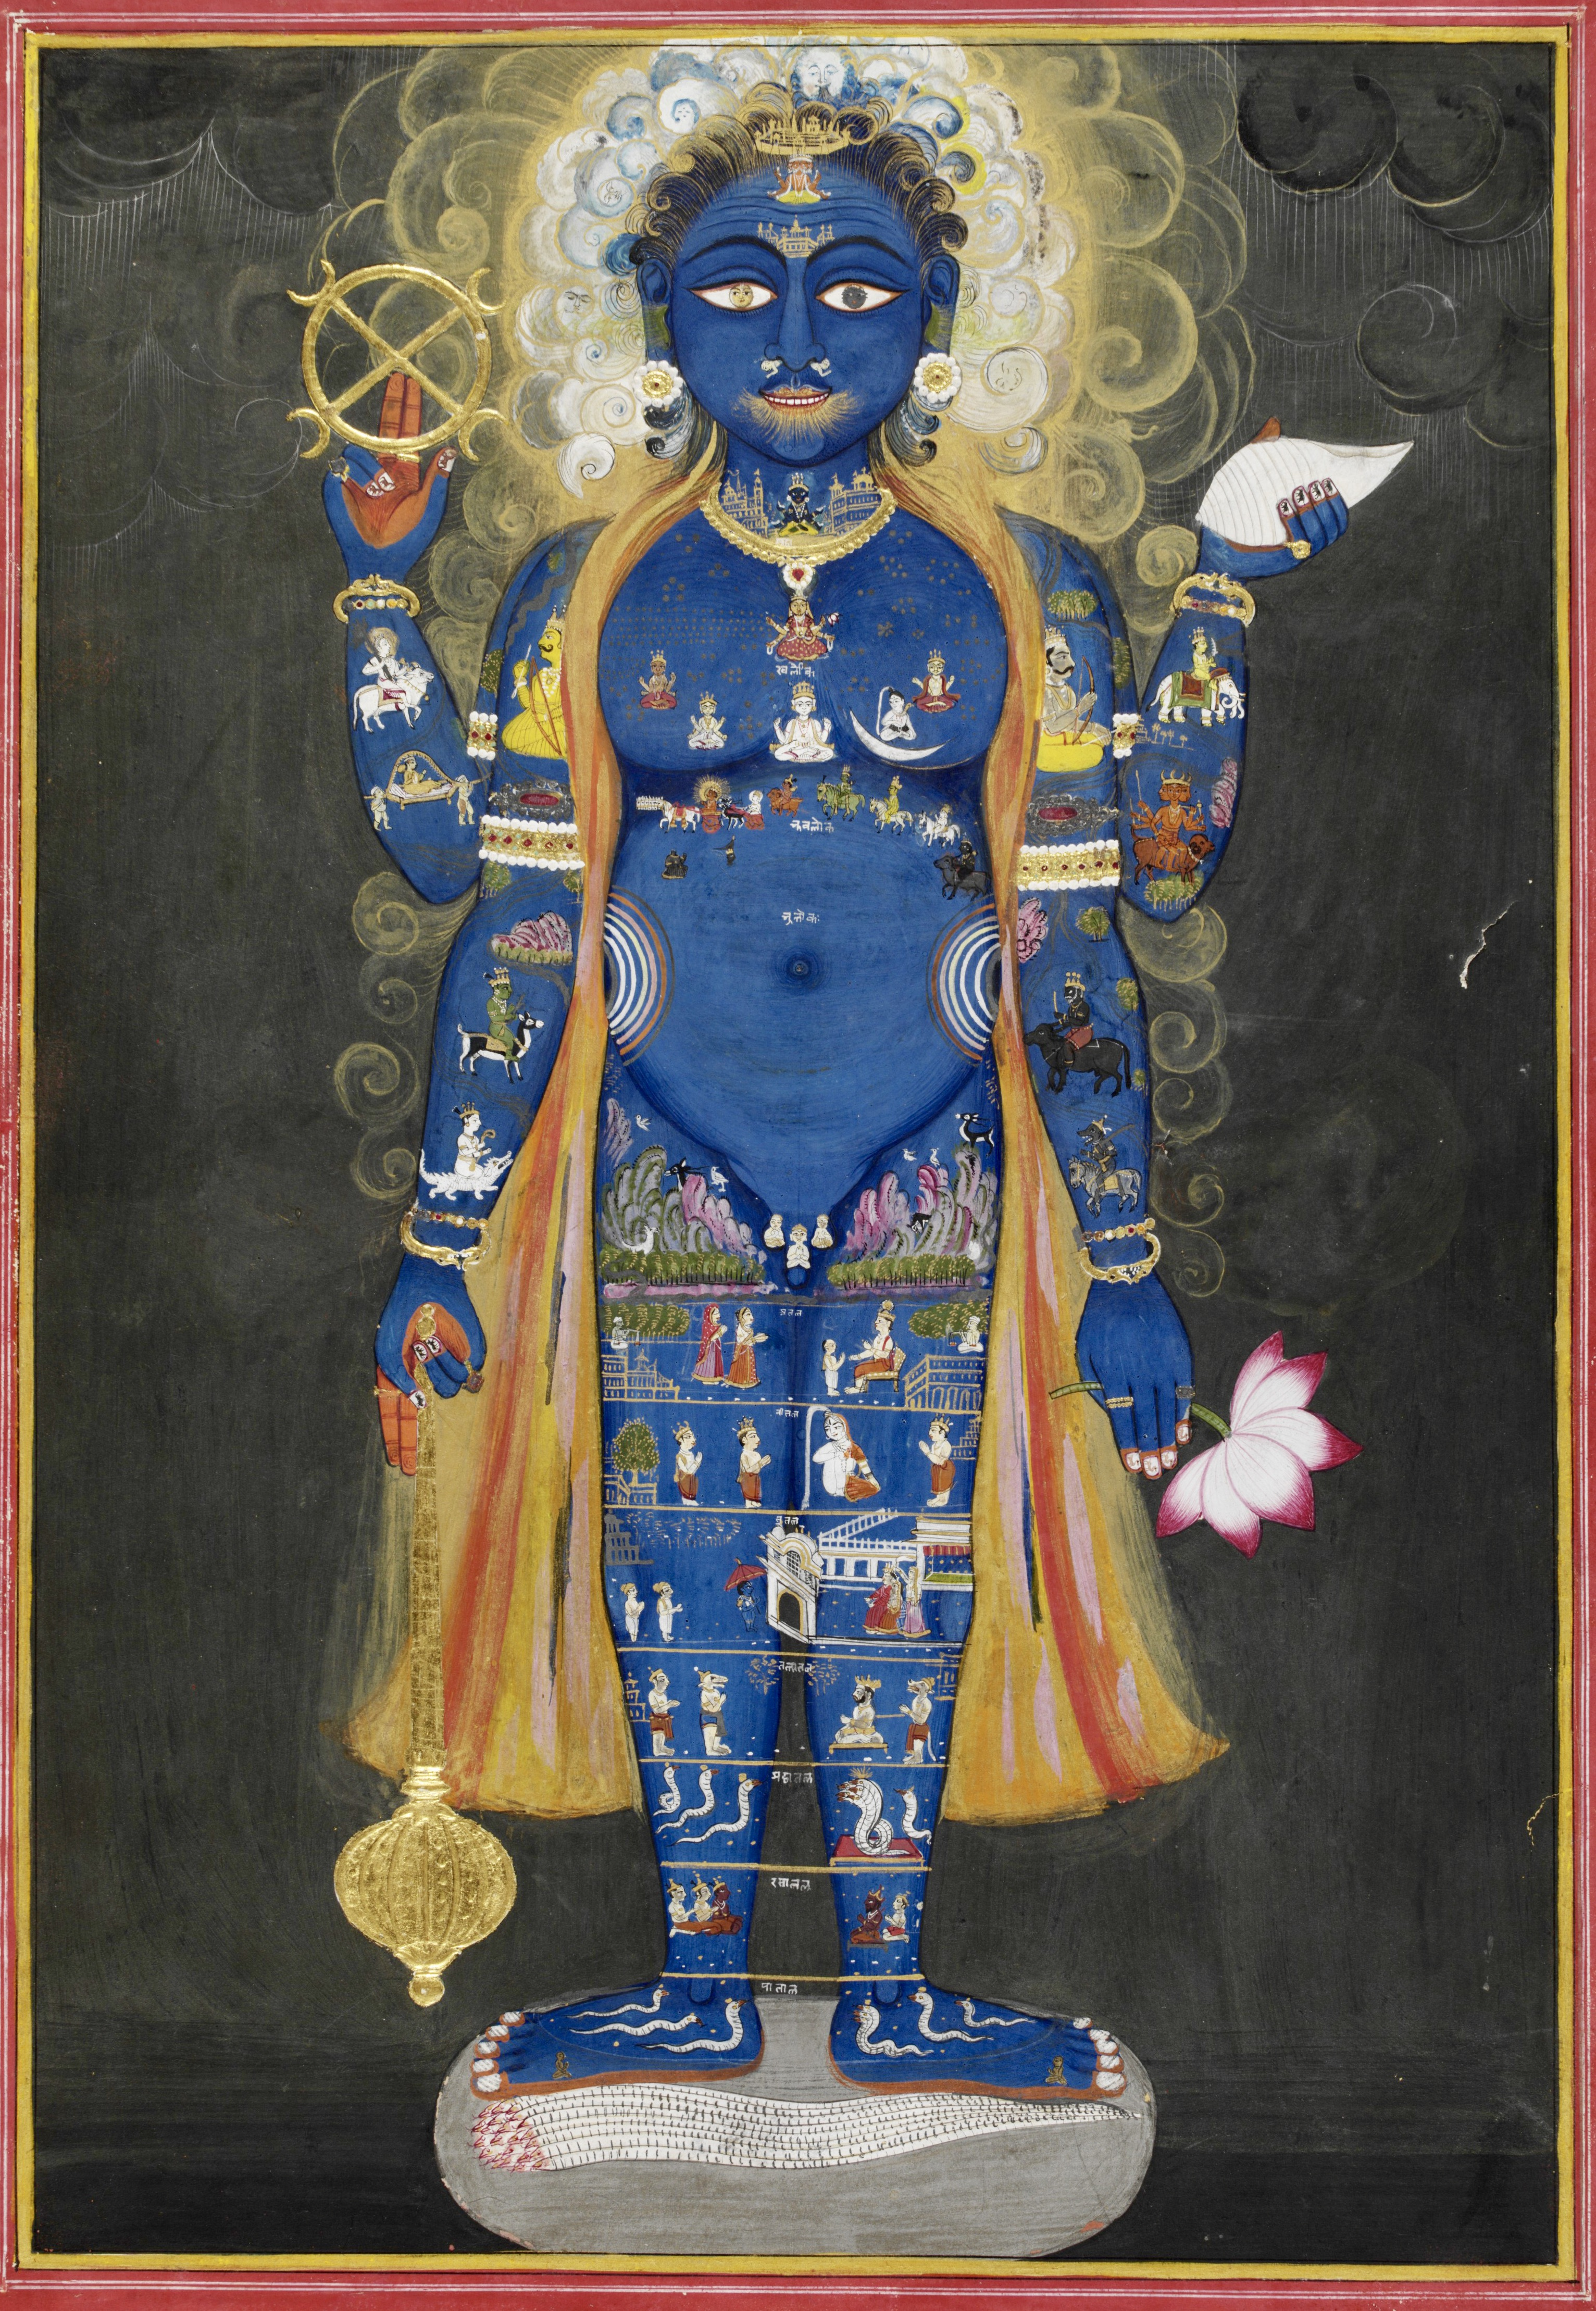
\includegraphics[width=1\textwidth]{pics/Vishnu_Vishvarupa_cropped.jpg}
	\caption{Viṣṇu Viśvarūpa, India, Rajasthan, Jaipur, ca. 1800–1820, Opaque watercolor and gold on paper, 38.5 × 28 cm, Victoria and Albert Museum, London, Given by Mrs. Gerald Clark.}
	\label{fig1}
      \end{figure}
\clearpage
  \begin{figure}[ht]
	\centering
  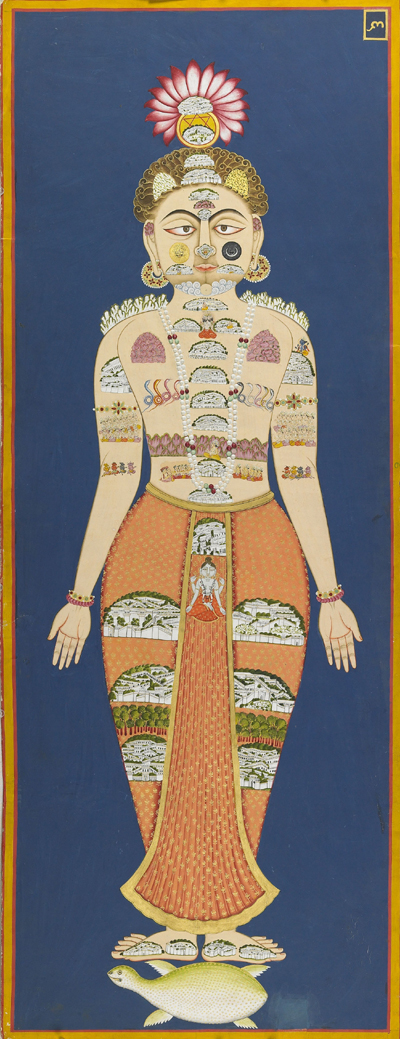
\includegraphics[width=0.5\textwidth]{pics/The_Equivalence_of_Self_and_Universe_(detail),_folio_6_from_the_Siddha_Siddhanta_Paddhati,_(Bulaki),_1824_(Samvat_1881);_122_x_46_cm._Mehrangarh_Museum_Trust..jpg}
	\caption{The Equivalence of Self and Universe (detail), folio 6 from the \textit{Siddhasiddhāntapaddhati} (Bulaki), India, Rajasthan, Jodhpur, 1824 (Samvat 1881), 122 x 46 cm, RJS 2378, Mehragarh Museum Trust.}
	\label{fig2}
      \end{figure}
      % \end{landscape}


\chapter{Bibliography}
 \label{sec:bibli}
   \clearpage
\newpage 
\thispagestyle{empty}
\quad  \addtocounter{page}{-1}

\printbibliography[heading=subbibintoc, title=Consulted Manuscripts, keyword=codex]

\printbibliography[heading=subbibintoc, title=Printed Editions, keyword=printsource]

\printbibliography[heading=subbibintoc, title=Secondary Literature, keyword=seclit]

\printbibliography[heading=subbibintoc, title=Online Sources, keyword=onlinesource]

\end{document}
